\documentclass[a4paper,twoside,12pt]{report}
\usepackage[pdftex]{graphicx}
\usepackage{tocloft}
%
\usepackage[smaller]{acronym}
\usepackage{amsfonts}
\usepackage{amsmath}
\usepackage{atlasphysics}
\usepackage{bbold}
\usepackage{booktabs}
\usepackage[pdftex,color]{changebar}
\usepackage{fancyhdr}
\usepackage{hyperref}
\usepackage{lineno}
\usepackage{mathrsfs}
\usepackage{multirow}
\usepackage{pdfpages}
\usepackage{sectsty}
\usepackage{setspace}
\usepackage{subfig}
\usepackage{type1cm}
\usepackage[normalem]{ulem}
\usepackage{url}
\usepackage{xspace}
%
\usepackage[Sonny]{fncychap} %Styles: Sonny, Lenny, Glenn, Conny, Rejne, Bjarne, and Bjornstrup.

\newcommand{\thesistitle}{Random collection of top, higgs and DECAL studies} %Fill in title
\newcommand{\thesisauthor}{A. Winter} %Fill in your name
\newcommand{\thesisemail}{aw@hep.ph.bham.ac.uk} %Fill in your email
%Choose your front page crest. crest_1 (photograph) or crest_2 (logo)
\newcommand{\thesiscrest}{crest_1}

\hypersetup{pdfpagelayout=TwoColumnRight,
            colorlinks,
            linkcolor=black,
            urlcolor=black,
            citecolor=blue,
            pdftitle={\thesistitle},
            pdfauthor={\thesisauthor},
            pdfsubject={High Energy Particle Physics Thesis},
            pdfcreator={\thesisemail}, 
}

%Set colour of change-bar
\cbcolor{red}

%Uncomment to add DRAFT watermark on every page
%\makeatletter
%\AddToShipoutPicture{%
%            \setlength{\@tempdimb}{.5\paperwidth}%
%            \setlength{\@tempdimc}{.5\paperheight}%
%            \setlength{\unitlength}{1pt}%
%            \put(\strip@pt\@tempdimb,\strip@pt\@tempdimc){%
%        \makebox(0,0){\rotatebox{45}{\textcolor[gray]{0.97}%
%        {\fontsize{6cm}{6cm}\selectfont{DRAFT}}}}%
%            }%
%}
%\makeatother

%%%%%%%%%%%%%%%%%%%%%% Page dimensions %%%%%%%%%%%%%%%%%%%%%
\allsectionsfont{\sf} %sectsty

\setlength{\parskip}{12pt}  % 12 pt = space between paragraphs
\setlength{\parindent}{0pt} % 0 pt  = indentation

\textwidth 15.0cm
\textheight 235mm
\footskip 10 mm

%5mm is nominal, add remove 4mm
\setlength{\oddsidemargin}{1mm}
\setlength{\evensidemargin}{9mm}

\addtolength{\topmargin}{0cm}

\topmargin=0mm
\headheight=15pt
\headsep=10mm
%%%%%%%%%%%%%%%%%%%%%% Page dimensions %%%%%%%%%%%%%%%%%%%%%

% References
\newcommand{\refeq}[1]{(\ref{#1})}
\newcommand{\reftab}[1]{Table~\ref{#1}}
\newcommand{\reftabs}[1]{Tables~\ref{#1}}
\newcommand{\reffig}[1]{Figure~\ref{#1}}
\newcommand{\reffigs}[1]{Figures~\ref{#1}}
\newcommand{\refsec}[1]{Section~\ref{#1}}
\newcommand{\refapp}[1]{Appendix~\ref{#1}}

% Put your shortcuts here
\newcommand{\invmicrobarn}{\ensuremath{\mu\textrm{b}^{-1}}\xspace}
\newcommand{\microbarn}{\ensuremath{\mu\textrm{b}}\xspace}
\newcommand{\invsqcminvs}{\ensuremath{\textrm{cm}^{-2}\textrm{s}^{-1}}\xspace}
\newcommand{\mus}{\ensuremath{\mu\textrm{s}}\xspace}
\newcommand{\mum}{\ensuremath{\mu\textrm{m}}\xspace}
\newcommand{\sqs}{\ensuremath{\sqrt{s} = 7}~\TeV\xspace}


\begin{document}

\begin{titlepage}
  \begin{center}
    {\huge\sc \thesistitle}\\
    \vspace{3.0cm}
    {\Large\bf \thesisauthor}\\
    \vspace{1.5cm}
    {\large\em Thesis submitted for the degree of}\\
    {\large\em Doctor of Philosophy}\\
    \vspace{1.5cm}
  \end{center}
  \begin{center}
    \resizebox{6cm}{!}{
    \includegraphics*{fig/\thesiscrest}}
  \end{center}
  \begin{flushleft}
    \hspace{7.5cm} Particle Physics Group, \\
    \hspace{7.5cm} School of Physics and Astronomy, \\
    \hspace{7.5cm} University of Birmingham. \\
    \vspace{1cm}
    \hspace{7.5cm} \emph{\today} \\
  \end{flushleft}
  \begin{center}
  \end{center}
\end{titlepage}

\setstretch{1} 
\thispagestyle{empty}%BLANK PAGE
~
\newpage
\thispagestyle{empty}%BLANK PAGE
~
\newpage

\pagenumbering{roman} %INTRO

\pagestyle{fancy} %Set up page style
\fancyfoot{} % clear all footer fields
\fancyhead{}
\fancyhead[RE]{\sf \slshape \rightmark \hspace{5mm} \thepage }
\fancyhead[LO]{\sf \thepage \hspace{5mm} \slshape \leftmark }

%%%%%%%%%%%%%%%%%%%%%% Preamble Formatting %%%%%%%%%%%%%%%%%%%%%
\setcounter{tocdepth}{3}
\setcounter{secnumdepth}{3}
\renewcommand\tocloftpagestyle{fancy}
\renewcommand\cftchapfont{\large\sf}
\renewcommand\cftsecfont{\normalsize \sf}
\renewcommand\cftsubsecfont{\small\sf}
\renewcommand\cftsubsubsecfont{\footnotesize \sf}
%
\renewcommand\cftchappagefont{\bfseries\sffamily}
\renewcommand\cftsecpagefont{\bfseries\sffamily}
\renewcommand\cftsubsecpagefont{\bfseries\sffamily}
\renewcommand\cftsubsubsecpagefont{\bfseries\sffamily}
%
\renewcommand\cftloftitlefont{\Huge\sf}
\renewcommand\cftlottitlefont{\Huge\sf}
\renewcommand\cfttoctitlefont{\Huge\sf}
%%%%%%%%%%%%%%%%%%%%%% Preamble Formatting %%%%%%%%%%%%%%%%%%%%%

%%%%%%%%%% Abstract %%%%%%%%%%
\chapter*{ABSTRACT}
%
Within the next few years a decision must be made by the global community on what type of high energy colliders should be built in the post LHC era. Here we present studies showing what might be achieved if a linear lepton collider such as \ac{CLIC} is chosen. Two physics studies are presented showing the precision achievable in the electroweak sector when operating at 1.4 TeV. Firsty the measurement of $\sigma_{H\nu\bar{\nu}} \times BR(H\rightarrow WW^*)$, an integral component for model independent Higgs measurements, is described using the semileptonic decay channel and is shown to yield a statistical precision of 1.3\% for 1.5 ab$^{-1}$ of data. A differential measurement of the top quark forward backward asymmetry is also performed as a probe of the electroweak form factors of the ttX vertex yielding a statistical precision of $\mathcal{O}$(1\%) for 1.5 ab$^{-1}$ of data. Lastly, the potential for using a novel design of a \ac{DECAL} at the \ac{ILC} is studied showing that an energy resolution of $\frac{\sigma_E}{E}=\frac{16.1\%}{\sqrt{E}} \oplus \frac{0.5\%}{E} \oplus 0.4\%$ can be achieved, similar to what is seen for the standard design choice, when using 30 $\mu m$ pitch pixels with a 12 $\mu m$ epitaxial thickness.

%
\clearpage
\chapter*{DECLARATION OF AUTHORS CONTRIBUTION}
%
The work presented here has been carried out within the \ac{CLIC} and \ac{CALICE} collaborations however all the work presented here is solely the authors own work unless otherwise stated. The two physics studies presented in Chapters \ref{Higgs Analysis} and \ref{chapter:topanalysis} were performed using the ILCSoft framework used for all analyses at \ac{ILC} and \ac{CLIC} and used event samples generated centrally by \ac{CLIC}, however the reconstruction and event selection techniques used were chosen and implemented by the author. The study related to the Higgs sector has already been published in a paper summarising the potential for Higgs measurements\cite{Abramowicz:2016zbo} at \ac{CLIC} and a similar paper showing the potential for top quark measurements that will include the results from Chapter \ref{chapter:topanalysis} is currently under review\cite{TopPaperDraft}.

For the work presented in Chapter \ref{sect:DECAL} the DigiMAPS package was used for adding additional levels of realism to the simulation studies. This package was originally developed by Anne-Marie Magnan as part of the \ac{CALICE} collaboration and was adapted by the author to change how pixel noise was implemented and to allow for variations in the threshold between pixels. This work is in the process of being written into a paper by the author.

%
\clearpage
\chapter*{ACKNOWLEDGEMENTS}
%
Science is hard, PhDs especially so. People think you can just lie under apple trees until you get hit on the head and see the world anew but that's a once in a generation thing. In reality the apple just leaves you dazed and confused with a bit of a sore head. For the rest of us, being a scientist means chiseling away at the cold opaque walls of human knowledge in the hope of finding something worthwhile with no knowledge of whether we're even digging in the right place. It's not a glamorous or quick affair. It is a slow frustrating process that often yields little result. That being said, without it we don't progress. We wouldn't have the internet, anitbiotics or even things like tv and film. Without it we won't ever take our first step on a different planet, we won't cure cancer and we won't have that which we can't even imagine yet. As a result I'm proud to have been a part of it. Even if this research never comes to anything I can be proud that I've been able to carve a tiny ``AW was here'' in the void of human ignorance. As such I'd like to thank all those who have helped me be a part of the process either by showing me how to progress or by keeping me from giving in to the frustration.  

First and foremostly I need to thank my supervisor, Nigel Watson, for agreeing to take on a man with little to no particle physics or programming knowledge to do a PhD which is based entirely on knowing particle physics and being able to programme. His dedication to always find time for everyone despite having a virtual army of students to deal with and his ability to always explain things in a way even I could understand is something I am truly grateful for. Similarly I would like to thank Tony Price for all his help along the way even when he was no longer even part of the department and had no obligation to do so. I would also like to show my appreciation to all the member of the CLICdp working group for the valuable insight they have provided on both the analyses I worked on.

While the people above have all helped me develop as a physicist I would also like to thank those who have kept me sane and made the office a fun place to be: Andy ``legs'' C, Richard, Matt, Mark, Andy F, Jam\'{e}s, Tim Tim Tim, Daniel ``The Brigadier'', Elliot, James, Jack, John, Rob, Russell, Dan, Gov, Nandish and Robbie. While there have been many great moments over the years I think some of the highlights must certainly be the creation of danger juice, snail racing in the office and the double success in the Bubble Chambers football tournament. 

Special mentions also go to the various eateries that have kept me fuelled throughout the PhD. In particular, Go Mex for providing an unhealthy amount of burritos to my diet, Dilshad for making the best curry in Birmingham and The Goose for simply being The Goose.

Lastly I want to thank my wife Alison for moving to Birmingham in the first place, her tolerance of my moaning about work when she's just finished several night shifts nursing and for all her love and support through all the years. 
%
\cleardoublepage
~
\vspace*{\fill}
\begin{center}
  \emph{Motto or dedication}
\end{center}
\vspace*{\fill}
\cleardoublepage

%%%%%%%%%% Abstract %%%%%%%%%%

\tableofcontents
\clearpage

\listoftables
\clearpage

\listoffigures
\clearpage

\chapter*{DEFINITIONS OF ACRONYMS}
\sectionmark{DEFINITIONS OF ACRONYMS}
\chaptermark{DEFINITIONS OF ACRONYMS}
\begin{acronym}
  \acro{HL-LHC}{High Luminosity Large Hadron Collider}
  \acro{LHC}{Large Hadron Collider
    \acroextra{\\Superconducting collider occupying the 27 km ring at CERN.}}
  \acro{QCD}{Quantum Chromodynamics}
\acro{SM}{Standard Model}
\acro{BSM}{Beyond the Standard Model}
\acro{HL-LHC}{High Luminosity Large Hadron Collider}
\acro{FCC}{Future Circular Collider}
\acro{CLIC}{Compact Linear Collider}
\acro{ILC}{International Linear Collider}
\acro{ILD}{International Large Detector}
\acro{SiD}{Silicon Detector}
\acro{CMOS}{Complimentary Metal-Oxide Semiconductor}
\acro{MAPS}{Monlithic Active Pixel Sensors}
\acro{EM}{Electromagnetic}
\acro{ECAL}{Electromagnetic Calorimeter}
\acro{HCAL}{Hadronic Calorimeter}
\acro{DECAL}{Digital Electromagnetic Calorimeter}
\acro{CMS}{Compact Muon Solenoid}
\acro{ATLAS}{A Toroidal LHC Apparatus}
\acro{CERN}{European Organisation for Nuclear Research}
\acro{TDR}{Technical Design Report}
\acro{CDR}{Conceptual Design Report}
\acro{IP}{Interaction Point}
\acro{BDS}{Beam Delivery System}
\acro{BS}{Beamstrahlung}
\acro{TPC}{Time Projection Chamber}
\acro{SIT}{Silicon Internal Tracker}
\acro{SET}{Silicon External Tracker}
\acro{FTD}{Forward Tracking Detector}
\acro{ETD}{Endcap Tracking Detector}
\acro{RF}{Radio Frequency}
\acro{RF}{Radio Frequency}
\acro{PFA}{Particle Flow Algorithm}
\acro{PFO}{Particle Flow Object}
\acro{BDT}{Boosted Decision Tree}
\acro{LEP}{Large Electron-Positron Collider}
\end{acronym}


\cleardoublepage
\pagenumbering{arabic}
\setstretch{1.5} %Officially should be line spacing 2. But I think it looks too ugly
%\linenumbers %Uncomment for line numbering

%%%%%%%%%% Chapters  %%%%%%%%%%
\chapter{INTRODUCTION}


\chapter{Theory}


\chapter{Experiments}


\chapter{Higgs Analysis}


\section{Introduction}
Define what the top asymmetry is, measurement at previous experiments(tevatron, LHC, b asymmetry at lep), significance of it in terms of EW form factors


\begin{figure}
  \centering
  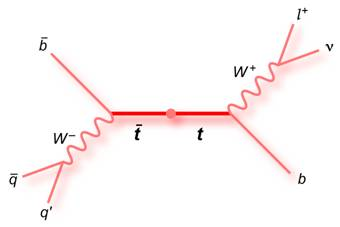
\includegraphics[width=0.5\textwidth]{figures/TopFeynmann.jpg}
  \caption[Semileptonic $t\bar{t}$ decay]{Semileptonic $t\bar{t}$ decay}
  \label{fig:topfeynmann}
\end{figure}

\begin{table}
  \centering
  \begin{tabular}{l |p{120mm}}
    \toprule
    Decay Mode     & Branching Fraction  \\
    \midrule
    $tt\rightarrow WbWb\rightarrow qqbqqb$ & \\
    \midrule
    $tt\rightarrow WbWb\rightarrow qqbql\nu b$ & \\
    \midrule
    $tt\rightarrow WbWb\rightarrow l\nu bl\nu b$ & \\
    \midrule
    $tt\rightarrow Other$ & \\
    \bottomrule
  \end{tabular}
  \caption{Top Pair Decay Modes}
  \label{table:topdecaymodes}
\end{table}


As tops decay almost exclusively to a W and b they are typically described in terms of the resulting decay modes of the Ws. The dominant decay modes are described in table \ref{table:topdecaymodes}. Here we will look at measuring $A_{FB}^{t}$ using the semileptonic $t\bar{t}$ decay channel (see figure \ref{fig:topfeynmann}) in which one. This decay mode is ideal as the lepton from the leptonically decaying top provides the ability to charge tag the tops while the fully hadronic decay allows an accurate measurement of the production angle of the tops, both of which are necessary for measuring $A_{FB}^{t}$ to high precision. The dominant signal and background processed examined by this analysis, as well as their cross sections and production ID numbers are shown in table \ref{table:topsamples}. All samples are simulated using the CLIC\_ILD\_CDR detector model. This is a variation of the ILD detector model developed for use at the ILC. The samples also include an overly of $\gamma\gamma\rightarrow$ hadron events from beamstralung based on a 30~ns window around the generated physics events. The dominant backgrounds are expected to be from alternative $t\bar{t}$ decays (fully hadronic decay modes and semileptonic decays containing taus) which will have very simliar topologies to the fact they will both contain a hadronically decaying top.

\begin{table}
  \centering
  \begin{tabular}{l | r | r |r}
    \toprule
    Process     & Cross Section(fb) & Production ID & Events Used  \\
    \midrule
    Signal: $ee\rightarrow t\bar{t}\rightarrow qqqql\nu$ & xx & 6589,6592,6634,6637 & xx \\
    \bottomrule
  \end{tabular}
  \caption{Top Pair Decay Modes}
  \label{table:topsamples}
\end{table}


\section{Event Reconstruction}
Reconstruction of the signal events is performed using ILCSOFT v01-17-10 and consists of three main stages. The first stage is to identify isolated leptons arising from the leptonically decaying top. These leptons are then removed and the remaining PFOs are resolved into two large radius ``fat jets''. These two fat jets must then be associated with either the b jet produced by the leptonically decaying top or to the combination of three jets arrising from the hadronically decaying top. A kinematic fitter is then used to reconstruct the neutrino and any ISR/Beamstrahlung photons present in the event.

\subsection{Lepton Finding}

Lepton finding is the first stage of reconstruction performed in each event. Due to the fact the measurement of $A_{FB}^{t}$ is entirely reliant on using the lepton charge to distinguish between top and antitop decays, it is essential that a high efficiency and purity are achieved and that there is no angular dependence on the performance. For this analysis lepton finding is done in two steps. Firstly, lepton candidates with energy > 10~GeV are identified using the particle ID provided by the Pandora Particle Flow Algorithm \cite{Thomson200925}. Only muons and electrons are examined due to the fact tau leptons require different reconstruction techniques to identify and are typicaly reconstructed with significantly lower efficiency. This first stage removes >90\% of fake candidates with negligible impact on efficiency. The second stage of lepton selection is to examine how isolated each of the candidates are. This is evaluated by resolving all PFOs in the event into five jets, then for each lepton candidate, measuring the energy of the candidate relative to the jet it was been associated with. For this process the ee kt algorithm was chosen for the jet finding to ensure that all lepton candidates are always placed within a jet. The lepton candidate found to have the highest ratio of $E_{Candidate}/E_{Jet}$ is then declared to be the isolated lepton arrising from the letonically decaying top. In the event that no lepton is selected by the first step, the restrictions on the particle ID and energy are relaxed and the lepton is selected purely based on which PFO is the most isolated according to step two. This method ensures that there is always exactly one lepton selected per event. The net efficiency with which this method selects a candidate with the correct charge is found to be 93\% for electrons and 96\% for muons.

As well as understanding the net efficiency for finding leptons it is also important to examine the angular dependence of the efficiency to ensure there is no bias that could effect the measurement of $A_{FB}^{t}$. Figure \ref{fig:netefficiency} shows how the efficiency varies with angle. The efficiency is seen to rapidly decline for $|Cos\theta| > 0.9$ due to detector acceptances. A decrease in efficiency is also seen for electrons at angles corresponding to the transition point between the ECAL barrel and endcaps. This effect is not seen for muons as they are also reconstructed using the muon detectors placed at a larger radius. Overall the efficiency is seen to be consistently worse for electrons than muons. This is to be expected as muons produce easily recognisable signatures in the detector due to the fact they typically penetrate through the tracker,ECAL,HCAL and muon sytems whereas electrons only leave deposits in the tracker and ECAL. In the case that tracks are lost during reconstruction or are wrongly associated to other PFOs it is then possible for photons to wrongly be labelled as electrons and vice versa leading to a higher fake rate for electrons.

\begin{figure}
  \centering
  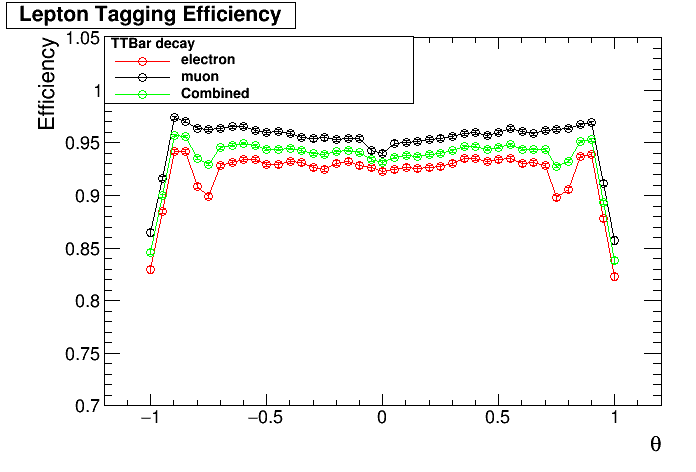
\includegraphics[width=0.6\textwidth]{figures/NetEfficiencys}
  \caption[Charge Tagging Efficiency]{Efficiency for identifying leptons with the correct charge as a function of angle}
  \label{fig:netefficiency}
\end{figure}

As well as checking the angular dependence of the charge tagging efficiency it is also key to examine the charge dependence of the lepton finding to make sure there is no preference for identifying particles over antiparticles. The angular dependence of the charge tagging efficiency for particles vs antiparticles is shown in figures \ref{fig:chargeEfficiencies}. An asymmetry in the performance is observed in both electrons and muons.

\begin{figure}
  \centering
  \begin{subfigure}{.5\textwidth}
    \centering
    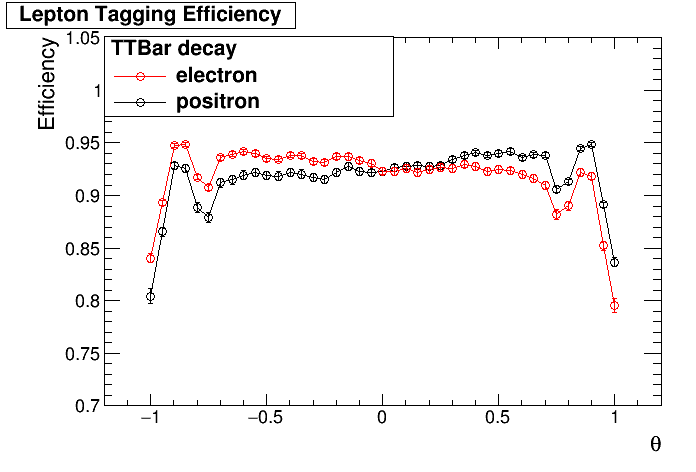
\includegraphics[width=0.9\textwidth]{figures/ElectronEfficiencys.png}
    \caption[Charge Tagging Efficiency]{Electrons}
    \label{fig:electronefficiency}
  \end{subfigure}%
  \begin{subfigure}{.5\textwidth}
    \centering
    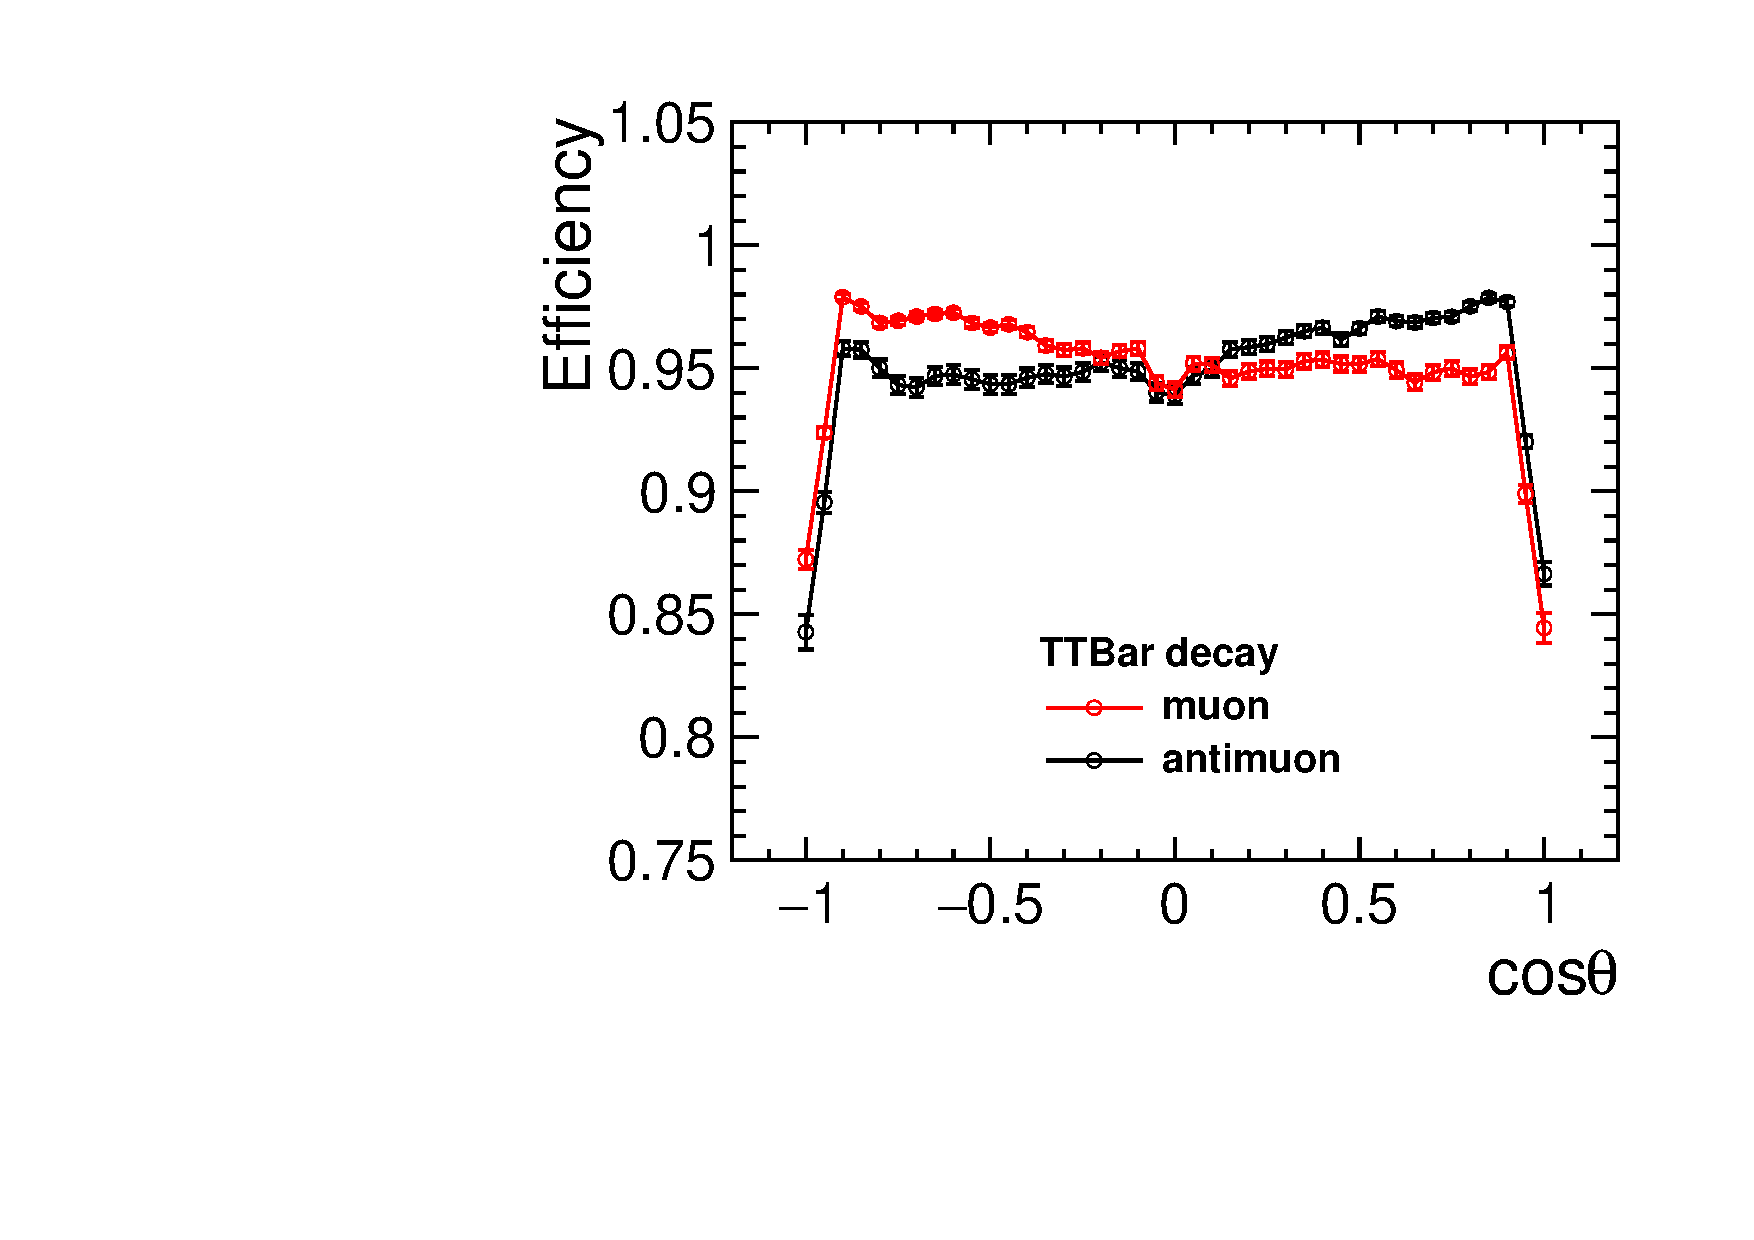
\includegraphics[width=0.9\textwidth]{figures/MuonEfficiencys}
    \caption[Charge Tagging Efficiency]{Muons}
    \label{fig:muonefficiency}
  \end{subfigure}
  \caption{Angular dependence of lepton finding for particles vs antiparticles}
  \label{fig:chargeEfficiencies}
\end{figure}

It arises from the underlying asymmetry in the production of particles vs antiparticles due to forward-backward asymmetries. The forward backward asymmetry mean that tops are preferencialy produced in one direction while antitops are produced more often in othe opposite direction, however due to charge conservation this also means that the W bosons and leptons are produced asymmetrically too. Because the collisions are taking place well above the top pair production threshold, the W bosons will gain a large boost forcing them to travel in the same direction as the inital top. The polarization of the W also means that the lepton will also be preferencially produced along the same diection as the W and can only be produced in the opposite direction with a lower energy. Overall this means that leptons are produced with higher energy in one direction and lower energy in the opposite direction while for antileptons this directional dependence is reversed. The effect is shown in \ref{fig:efficiency2d} where it is seen that positrons are produced with higher energy in the forward direction($cos\theta>0$) than the backward direction. It is known that the efficiency for reconstructing leptons at CLIC increases with energy and so the fact the energy and angle at which leptons are produced are correlated results in the asymmetric angular efficiency for correctly reconstructing the lepton. Further evidence for this theory is shown in figures \ref{fig:higgsleptons} and\ref{fig:effienciesWithCuts} which show that the asymmetry disappears when either the production mode for the leptons is symmetric or when low energy leptons are not included.

\begin{figure}
  \centering
  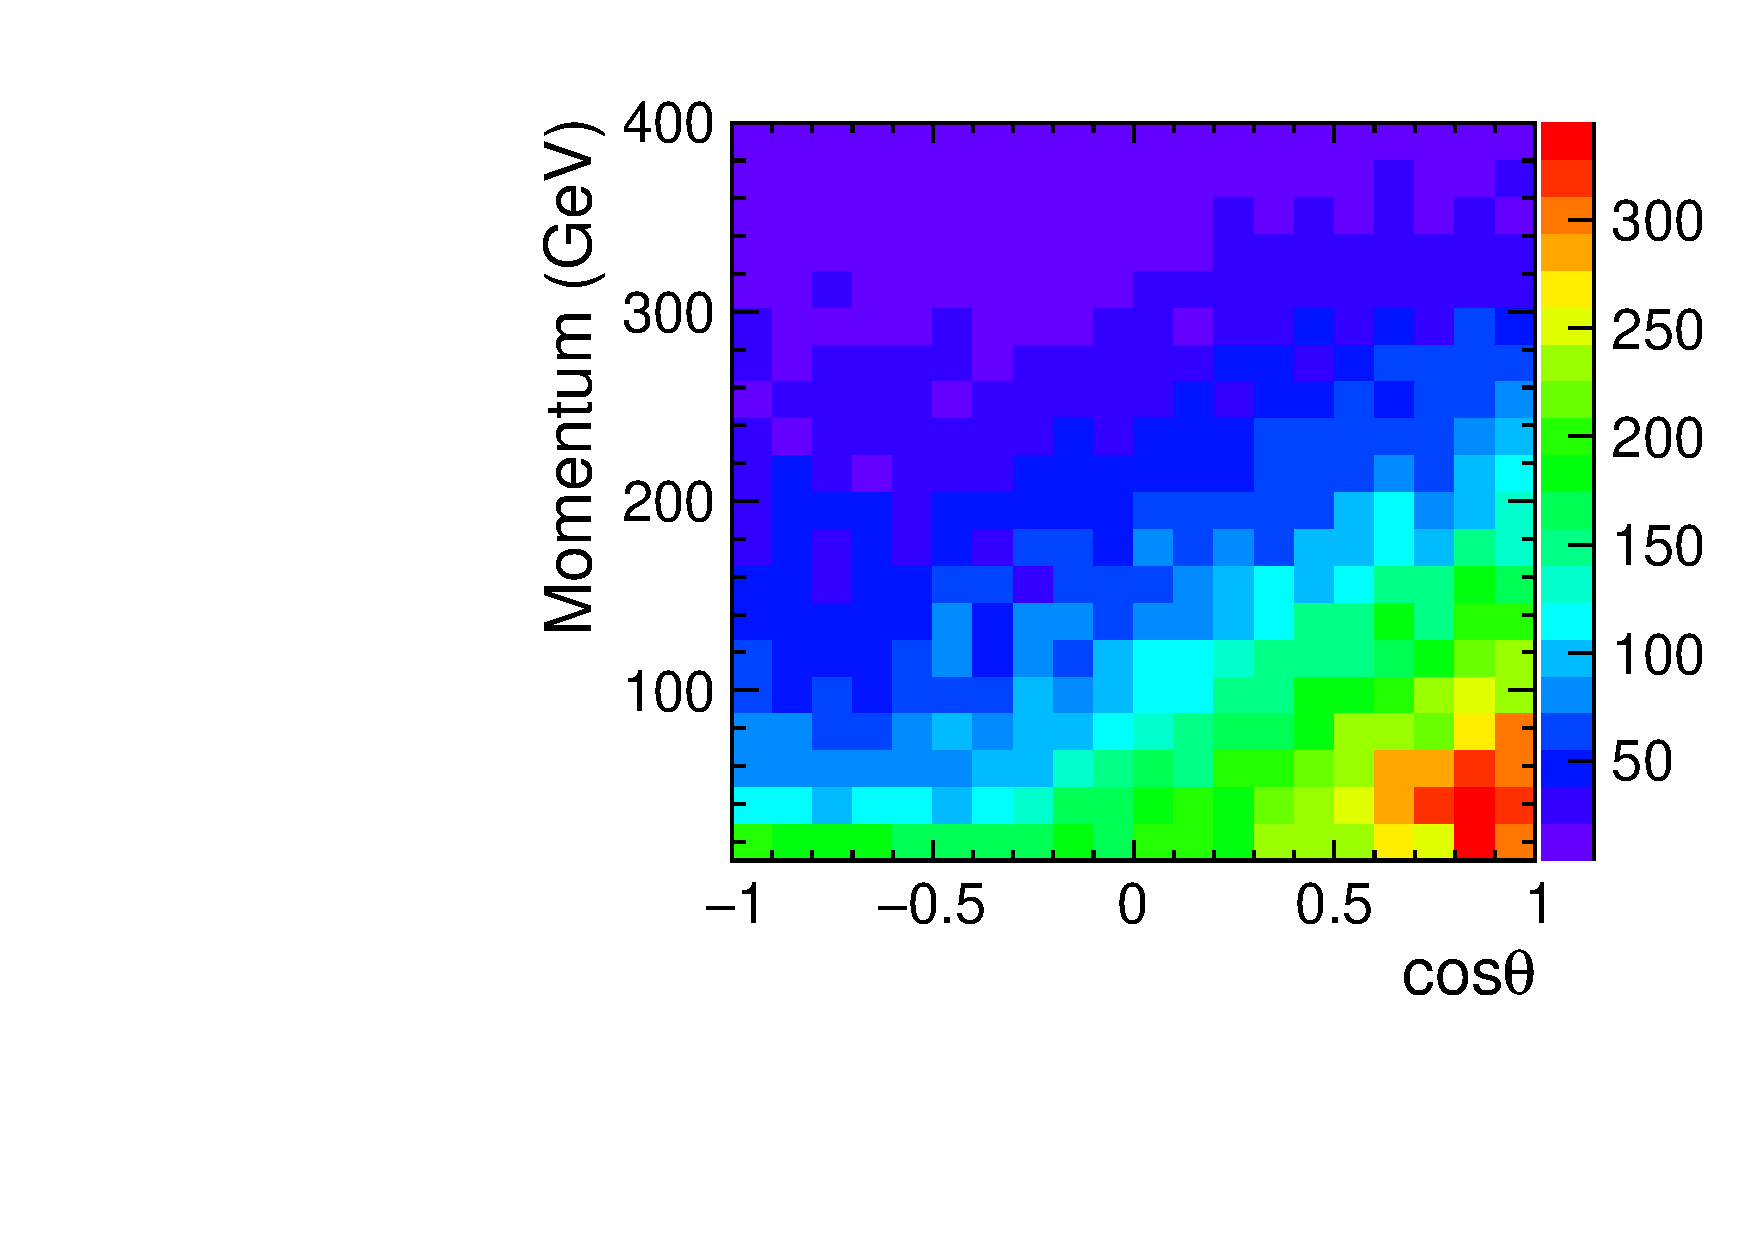
\includegraphics[width=0.6\textwidth]{figures/MomentumVsTheta}
  \caption[Lepton Momentum Vs Angle]{Correlation between lepton momentum and angle for positrons only}
  \label{fig:efficiency2d}
\end{figure}

\begin{figure}
  \centering
  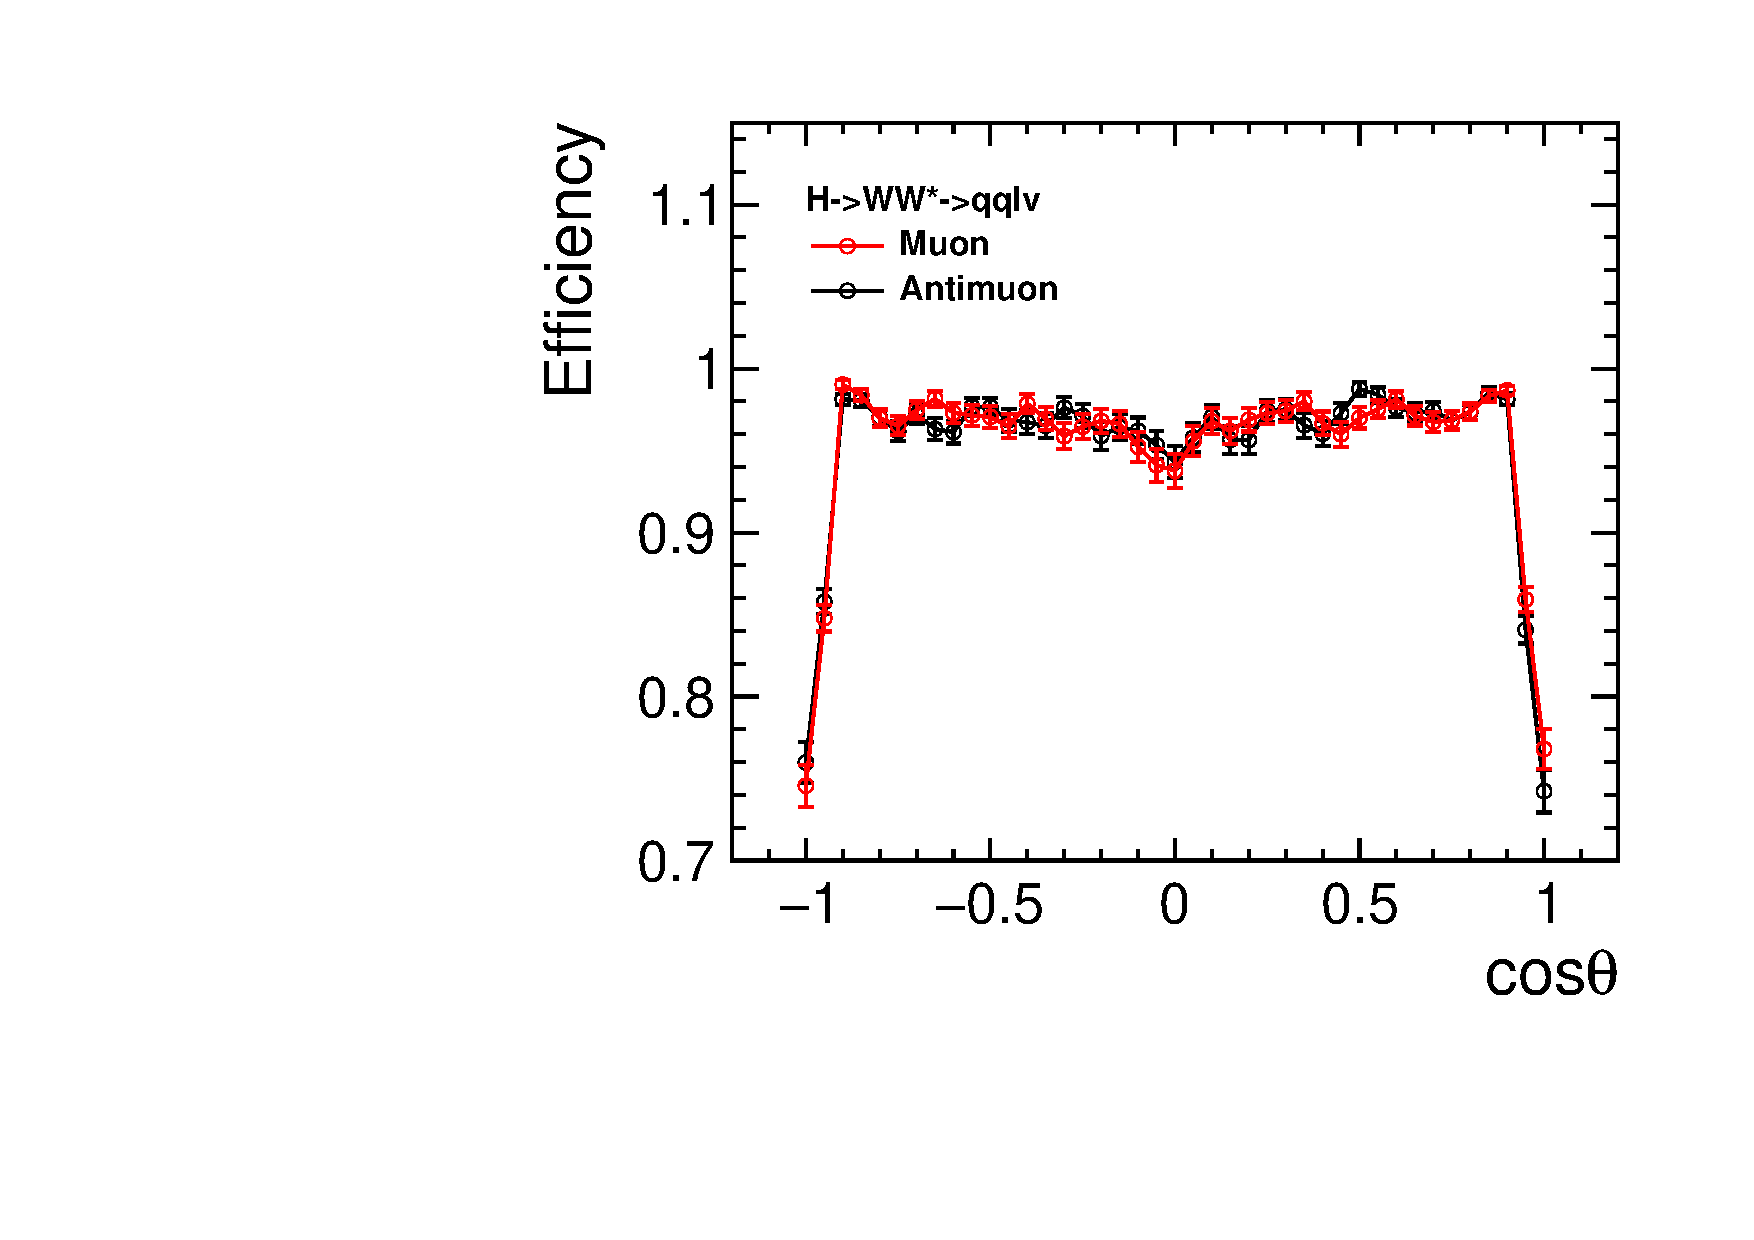
\includegraphics[width=0.6\textwidth]{figures/MuonEfficiency_Higgs}
  \caption[Lepton efficiency for $ee\rightarrow H\nu\nu,H \rightarrow WW\rightarrow qql\nu$ ]{Charge tagging efficiency for $ee\rightarrow H\nu\nu,H \rightarrow WW\rightarrow qql\nu$. The efficiency is seen to be symmetric for particles and antiparticles when they are produced with the same initial angular distribution.}
  \label{fig:higgsleptons}
\end{figure}

\begin{figure}
  \centering
  \begin{subfigure}{.5\textwidth}
    \centering
    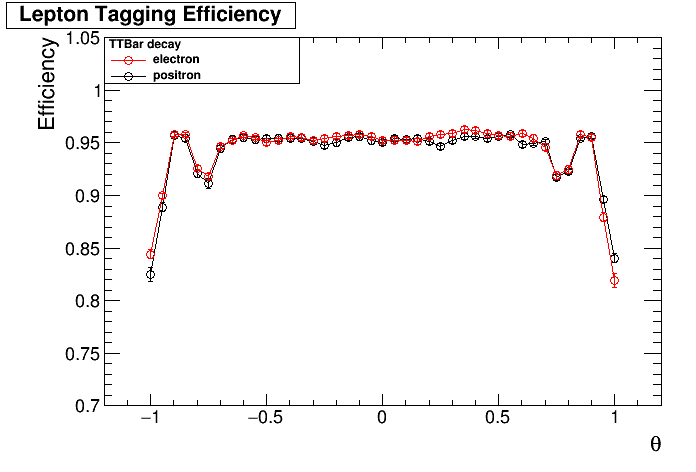
\includegraphics[width=0.9\textwidth]{figures/ElectronEfficiencys_20GeVCut.png}
    \caption[Charge Tagging Efficiency]{Electrons}
  \end{subfigure}%
  \begin{subfigure}{.5\textwidth}
    \centering
    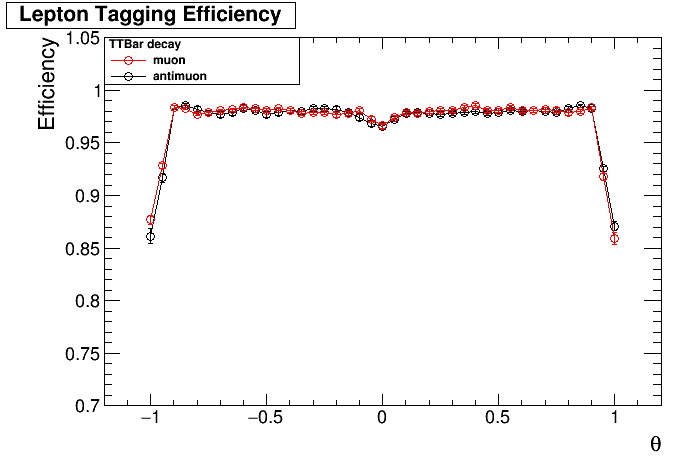
\includegraphics[width=0.9\textwidth]{figures/MuonEfficiencys_20GeVMCCut.png}
    \caption[Charge Tagging Efficiency]{Muons}
  \end{subfigure}
  \caption[Charge Tagging Efficiency After 20GeV Lepton Momentum Cut]{Charge tagging efficiency after 20~GeV lepton momentum cut. The efficiency is seen to be symmetric for leptons with momentum > 20~GeV/}
  \label{fig:effienciesWithCuts}
\end{figure}


\subsection{Fat Jet Finding}

\begin{figure}
  \centering
  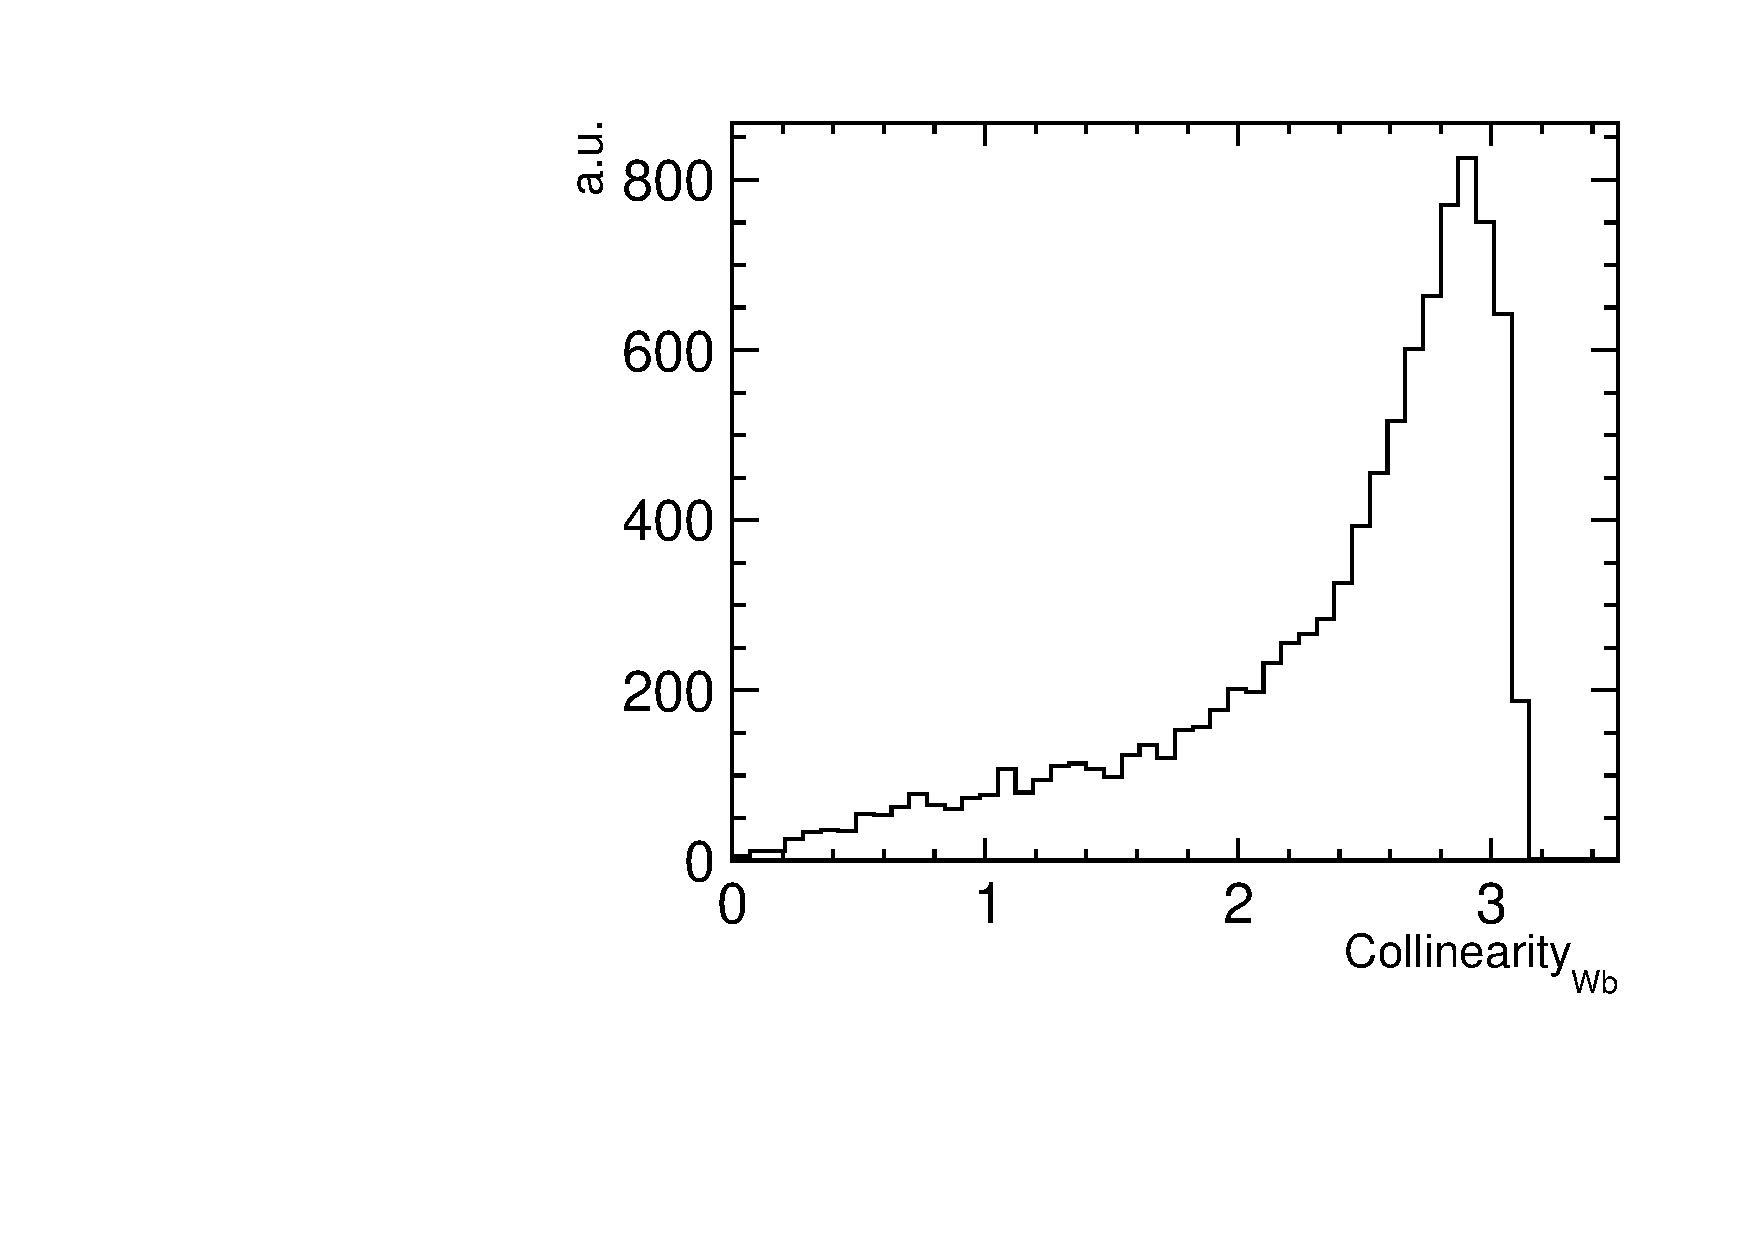
\includegraphics[width=0.6\textwidth]{figures/WBCollinearity}
  \caption[Separation between W and b jet from top decay]{Separation between W and b jets from top decay. The pair are typically too collimated to allow the b-jet and the pair of jets from the W decay to be successfully resolved into three distinct jets}
  \label{fig:Collimated}
\end{figure}

Jet reconstruction was performed using the FastJet package \cite{Cacciari:2011ma}. Due to the high energy of the collisions relative to the top mass, the tops produced are highly boosted and produce highly collimated decay products (see figure \ref{fig:Collimated}.) This means it is typically not possible to resolve the decay products from the hadronically decaying top into three jets corresponding to the b-jet and light quark jets from the W decay. As a result an alternative approach to jet reconstruction is considered based on the concept of fat jets, an approach already being used at the LHC\cite{Miller:2011qg}. Fat jets are large radius jets and are used to cluster groups of jets that can't be accurately resolved individually into one larger jet. For the purpose of this anaylsis the events are clustered into fat jets which should correspond to the b-jet from the leptonically decaying top and to the whole set of decays products from the hadronically decaying top. The mass and substructure variables (see \ref{Event Selection}) of these fat jets can then be used to distinguish genuine top events from backgrounds. Two jet algorithms were considered for reconstructing the fat jets- the kt algorithm \cite{Cacciari:2008gp} and Valencia algorithm \cite{Boronat:2014hva}. The kt algorithm is already extensively used at hadron colliders while the Valencia algorithm is a newer algorithm designed for future lepton colliders that offers improved performance in handling beam backgrounds. The performance of both algorithms is shown in figure \ref{fig:jetfinding}. For both algorithms it is seen that at higher R the resolution on the top mass gets worse while for lower R sub peaks start to appear in the mass distribution corresponding to partial reconstructions of the top (either W Boson or single quark). The kt algorithm is seen to produce a consistently broader distribution in the top mass. Placing a cut on the collision energy of E>1.2~TeV reveals that these lower mass peaks only occur for lower collision energies where the top decay products will be less collimated and so the fat jet finding can merge components from both the hadronic and leptonic tops into each jet. This analysis will be focusing on reconstructing the most boosted tops. As a result the Valencia algorithm is preferred due to it's better mass resolution. Performance for less boosted top decays might be improved by examining the performance of a more conventional jet analysis looking to resolve all four individual quarks whenever the fat jet finding produces jets outside the top mass window. This possibility is discussed later in section \ref{Quality Cuts}. Here the Valencia algorithm with R=1.5, $\beta$=1 and $\gamma$=1 is chosen as the optimal jet reconstrcution method to provide a balance between mass resolution and the frequency of partial reconstructions. 

\begin{figure}
  \centering
  \begin{subfigure}{.5\textwidth}
    \centering
    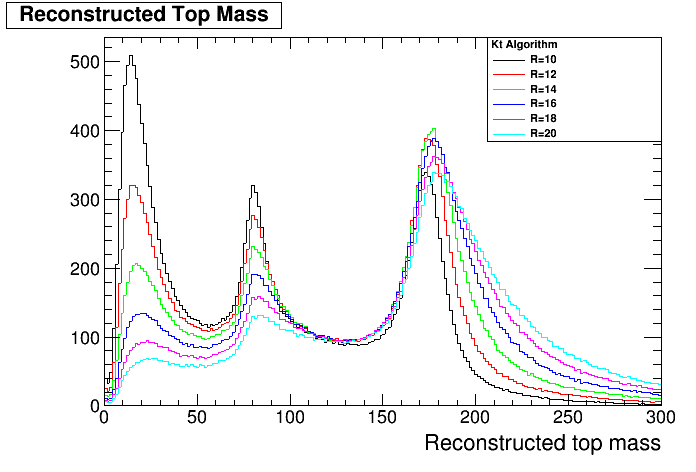
\includegraphics[width=0.9\textwidth]{figures/ComparisonKt.png}
    \caption[kt-alogorithm]{kt-algorithm}
  \end{subfigure}%
  \begin{subfigure}{.5\textwidth}
    \centering
    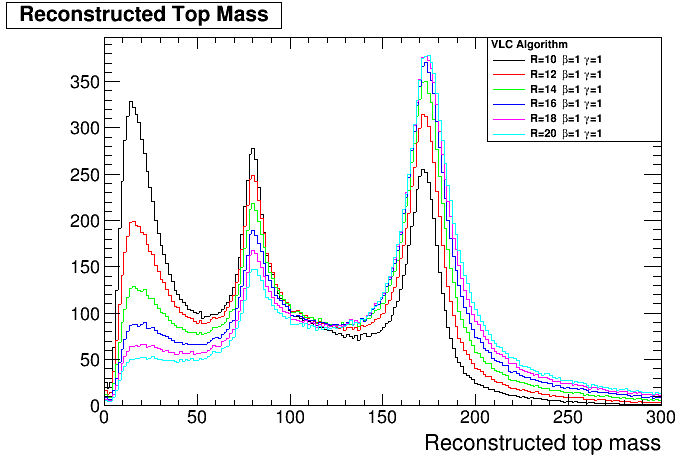
\includegraphics[width=0.9\textwidth]{figures/ComparisonVLC.png}
    \caption[Valenica algorithm]{Valencia}
  \end{subfigure}
  \caption[Performance of jet finding algorithms]{Performance of both jet finding algorithms for various parameter settings. The kt algorithm is seen to produce a broader distribution in the top mass peak so the Valencia algoritm is prefered. For both methods it is seen that a lower R results in the development of peaks from partial reconstruction of the top jet (W Boson or single quark) while a larger R produces a broader peak at the top mass. A balance is found between producing a narrow top mass width while minimising sub peaks by selecting a radius of R=1.5 }
  \label{fig:jetfinding}
\end{figure}


\begin{figure}
  \centering
  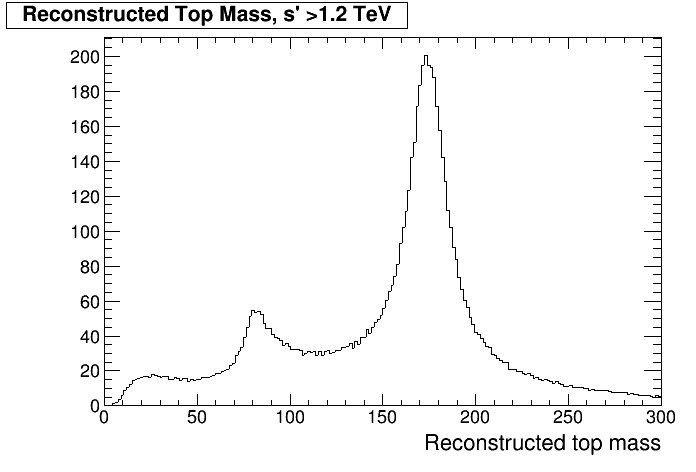
\includegraphics[width=0.4\textwidth]{figures/TopMass_EOver1200.png}
  \caption[Performance of Valencia algorithm for high energy events]{Reconstructed top mass for the Valencia algorithm in events close to the nominal collison energy (E>1.2~TeV)}
  \label{fig:highEValencia}
\end{figure}


\subsubsection{Jet Association}

\begin{figure}
  \centering
  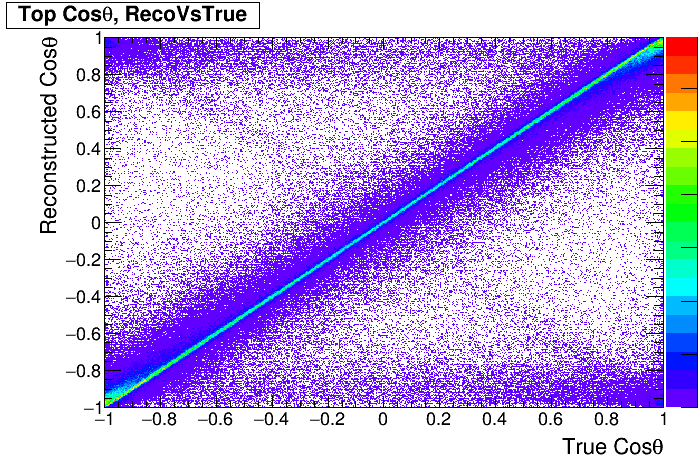
\includegraphics[width=0.4\textwidth]{figures/CosThetaRecoVsMC.png}
  \caption[Comparison of reconstructed top decay angle to truth]{Comparison of reconstructed top decay angle to truth. A strong correlation is seen over most of the range, however this starts to break down for large angles of $\mid Cos\theta \mid>0.9$ where non-negligible off diagonal contributions are seen.}
  \label{fig:2djetangle}
\end{figure}

\begin{figure}
  \centering
  \begin{subfigure}{.5\textwidth}
    \centering
    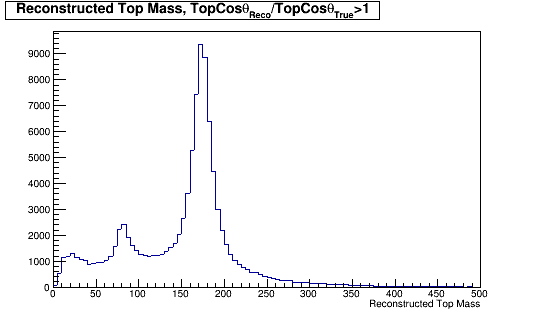
\includegraphics[width=0.9\textwidth]{figures/TopMassDiagonal.png}
    \caption[$\mid\frac{Cos\theta_{Reco}}{Cos\theta_{True}}\mid >1$]{Fat jet mass when $\mid\frac{Cos\theta_{Reco}}{Cos\theta_{True}}\mid >1$, on diagonal regions of fig \ref{fig:2djetangle}.}
  \end{subfigure}%
  \begin{subfigure}{.5\textwidth}
    \centering
    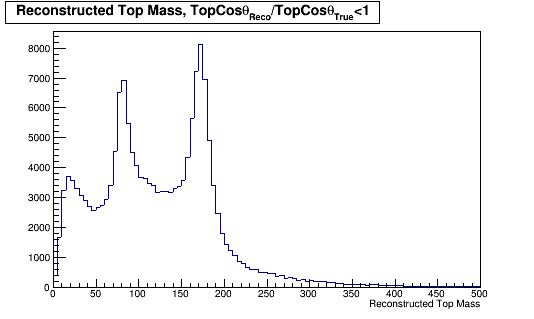
\includegraphics[width=0.9\textwidth]{figures/TopMassOffDiagonal.png}
    \caption[$\mid\frac{Cos\theta_{Reco}}{Cos\theta_{True}}\mid >1$]{Fat jet mass when $\mid\frac{Cos\theta_{Reco}}{Cos\theta_{True}}\mid <1$, off diagonal regions of fig \ref{fig:2djetangle}.}
  \end{subfigure}
  \caption[Reconstructed fat jet mass]{Reconstructed fat jet mass. In the regions where $\mid\frac{Cos\theta_{Reco}}{Cos\theta_{True}}\mid >1$ (upper right and lower left quadrants of fig \ref{fig:2djetangle}) the reconstructed fat jet matches the top mass, while in the regions corresponding to the off diagonal regions of fig \ref{fig:2djetangle}) the mass is not consistent}
  \label{fig:diagonalTopMass}
\end{figure}


After the fat jet finding has been performed, the two reconstructed jets must then be associated as either coming from the hadronically decaying top or from the b jet from the leptonically decaying top. The default method for this was to associate the highest energy fat jet to the hadronically decaying top as, due to the neutrino not being reconstructed and the lepton already being removed, the remaining decay products from the leptonically decaying top should typically have considerably less energy. The performance of this method can be examined by comparing the reconstructed decay angle relative to the true value(see \ref{fig:2djetangle}). While the performance over most of the range studied is good, for $\mid Cos\theta \mid>0.9$ the correlation between the true and reconstructed angles breaks down and off diagonal elements start to appear. Performance in these forward regions is typically poor due to detector acceptances which result in losses down the beam line. In cases where parts of the hadronic top decay are not able to be reconstructed, using the fat jets energy to perform the jet association no longer becomes a reliable method. Evidence that misreconstruction is the source of these off diagonal elements is presented in figure \ref{fig:diagonalTopMass} where it is clear that the fat jets in the off diagonal regions are not reconstructed with a consistent mass. When the jets are not fully reconstructed, it is more likely that the wrong jet is assigned to be from the hadronic top. When the wrong jet is selected the reconstructed angle will be approximately $\pi$ radians off the true value as the tops are predominantly produced back to back. This explanation is further supported by the results shown in figure \ref{fig:2djetangle_farfromleptop} which show that the off diagonal elements can be removed when a cut is placed on the angle between the reconstructed top and the b jet from the leptonic top decay indicating that these elements are definitely coming from selecting the wrong jet. As well as the $\pi$ radian flips from selecting the wrong jet, there are also additional off diagonal contributions seen which arise from poor reconstruction of the fat jets. This typically happens when the tops are not produced back to back due to ISR/Beamstrahlung. When this happens, during the fat jet reconstruction it is possible for contributions from both true fat jets to be mixed e.g instead of grouping the 3 jets from the hadronic jets together only two of them are grouped together and the third is grouped with the lone bjet from the leptonic top. When this mismatching happens the hadronic top is no longer fully reconstructed and so the angle measured for the top decay has little correlation with the true value. Figure \ref{fig:2djetangle_goodtopseparation} shows that these remaining off diagonal elements disappear when a cut is placed on the separation of the tops at truth level. 

\begin{figure}
  \centering
  \begin{subfigure}{.5\textwidth}
    \centering
    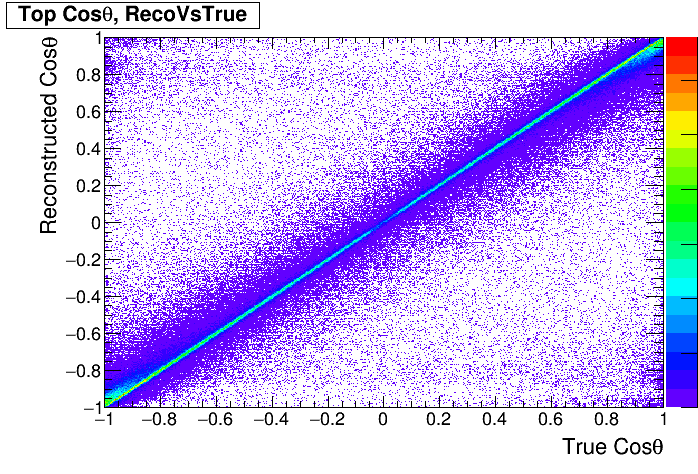
\includegraphics[width=0.9\textwidth]{figures/CosThetaRecoVsMC_NotNextToLepTop.png}
    \caption[Cut placed on angle between reconstructed top and true b jet from leptonic decay]{Cut placed on angle between reconstructed top and true b jet from leptonic decay, $\Delta Cos\theta_{Reco-Bjet}>0.1$}
    \label{fig:2djetangle_farfromleptop}
  \end{subfigure}%
  \begin{subfigure}{.5\textwidth}
    \centering
    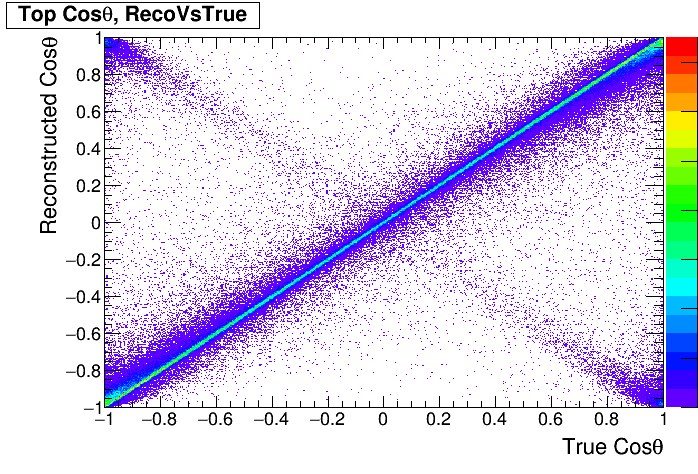
\includegraphics[width=0.9\textwidth]{figures/CosThetaRecoVsMC_MCTopsWellSeparated.png}
    \caption[Cut placed on collinearity between top pair at truth level]{Cut placed on collinearity between top pair at truth level, separation > 3 radians}
    \label{fig:2djetangle_goodtopseparation}
  \end{subfigure}
  \caption[Reconstructed vs true top decay angles with truth level cuts]{Reconstructed vs true top decay angles with truth level cuts to explain the off diagonal elements seen in \ref{fig:2djetangle}.}
  \label{fig:2djetangle_explanations}
\end{figure}




In order to avoid the problems close to the beam line multiple alternative jet association methods were devised- see \ref{fig:methodDescription}.
\begin{table}
  \centering
  \begin{tabular}{l |p{120mm}}
    \toprule
    Fat Jet Selection Method     & Description  \\
    \midrule
    Lepton & The hadronically decaying top is deemed to be the fat jet with the greatest separation from the isolated lepton\\
    \midrule
    B tag & The hadronically decaying top is deemed to be the fat jet with the greatest separation from the jet with the highest b tag (see \ref{Flavour Tagging} for details on how flavour tagging is performed)\\
    \midrule
    Energy & Select the fat jet with the highest energy to be the hadronically decaying top\\
    \midrule
    Multiplicity & Recluster both fat jets into N ``micro jets'' (see \ref{Jet Multiplicity} for methodology) The hadronically decaying top should have a higher number of micro jets found within it\\
    \midrule
    Mass & The hadronically decaying top is deemed to be the fat jet with the greatest mass \\
    \midrule
    Top Mass & Select the fat jet whos mass is closest to the top mass as the hadronically decaying top\\
    \midrule
    Democratic & A combination of the lepton, energy and mass methods. Each method votes for which fat jet it thinks is the hadronically decaying top. The fat jet with the most votes is then selected as the hadronically decaying top  \\
    \bottomrule
  \end{tabular}
  \caption{Methods used for identifying which fat jet corresponds to the hadronically decaying top}
  \label{fig:methodDescription}
\end{table}

The relative effectiveness of these methods were evaluated in three ways shown in figures \ref{fig:methodComparison}, \ref{fig:angleFitDiff} and \ref{fig:angularEfficiency} respectively. The first method was to look at the overall distribution of Cos$\theta$ produced by each method compared to the distribution at truth level as this is what will be used to extract $A_{fb}^{t}$. All the methods agree well with the true distribution in the central region of the detector but diverge in the high $\mid Cos\theta\mid$ region. This is mainly caused by the effect described above. Close to the beam line the jets aren't fully reconstructed, the jet assoication fails and the b jet from the leptonic side is selected rather than the hadronic top jet. This causes migrations from the forward region to the backward regions producing a deficit in the foward region and an excess in the backward region. Migrations do occure in the opposite direction too for the same reason, however because the top forward-backward asymmetry means tht more tops are produced in the forward region to begin with, the net migration is from forward to backward. The migrations are not always a shift of $\pi$ radians as one might expect. Instead the migrations occur from very close to the beam line to a broader range in the opposite direction. This is due to the fact that ISR/Beamstrahlung can mean the top pair aren't produced exactly back to back in the lab frame and because the b-jet produced by the leptonic decay is not exactly collinear with the the top decay axis. Comparing the methods we see that all the methods show similar levels of migration except for the btag method which shows the highest migration. This is attributed to the fact the highest btagged jet can sometimes be from the hadronic side even in events that are well reconstructed, and so the jet association will fail in more events than the other methods which only fail for events close to the beam line.

\begin{figure}
  \centering
  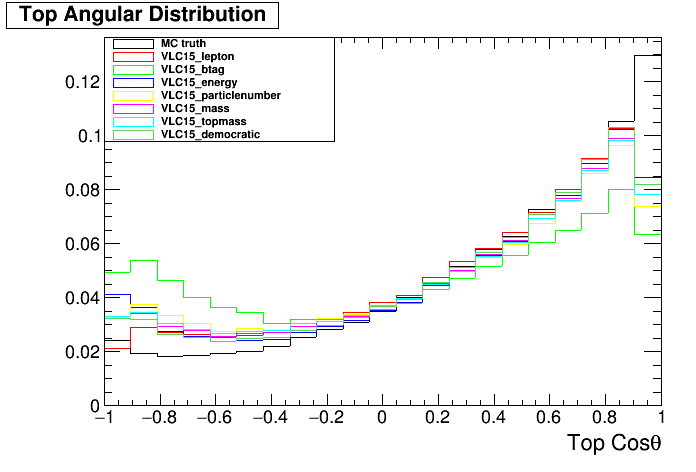
\includegraphics[width=0.6\textwidth]{figures/comparejetmethods.png}
  \caption[Reconstructed Cos$\theta$ distribution for various jet association methods]{Reconstructed Cos$\theta$ distribution for various jet association methods. The expected distribution from truth level information is uncluded for reference}
  \label{fig:methodComparison}
\end{figure}

The second method was to measure the difference between the reconstructed and MC(true) Cos$\theta$ per event and fit this with a gaussian. The variation in the width and mean of these distributions were plotted against the true Cos$\theta$ and are shown in fig \ref{fig:angleFitDiff}. The effects of migration at high Cos$\theta$ is more pronounced in these plots where in the width we can see that the resolution on Cos$\theta$ gets much worse in the forward regions and the mean shows a pull in opposite directions in these regions proving the migrations do indeed occur in both directions with the same. Unfortunately there is little discrimination seen between the methods except for showing that there are slightly larger migrations when using the btag method.

\begin{figure}
  \centering
  \begin{subfigure}{.5\textwidth}
    \centering
    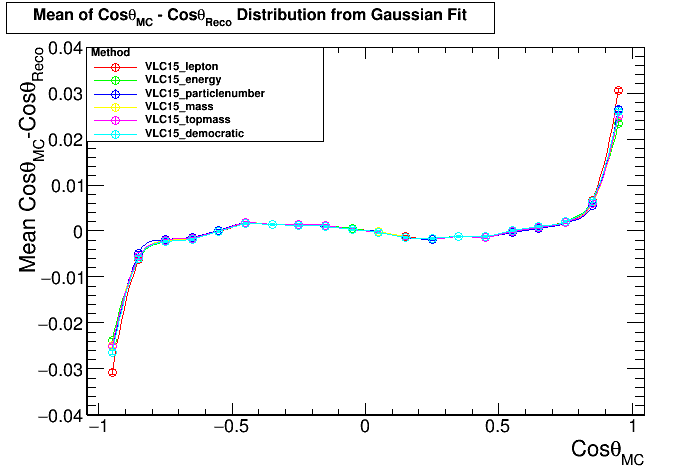
\includegraphics[width=0.9\textwidth]{figures/MeanThetaDiff.png}
    \caption[Mean]{Mean}
  \end{subfigure}%
  \begin{subfigure}{.5\textwidth}
    \centering
    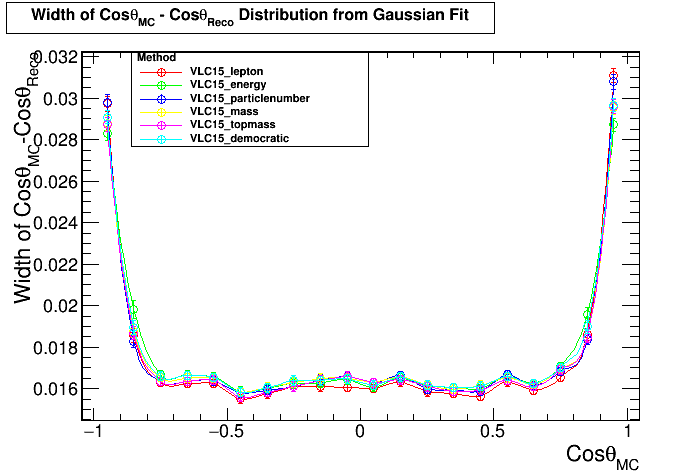
\includegraphics[width=0.9\textwidth]{figures/WidthThetaDiff.png}
    \caption[Width]{Width}
  \end{subfigure}
  \caption[Mean and width from fitting $\Delta Cos\theta_{True-Reco}$ to a gaussian]{Mean and width from fitting $\Delta$Cos$\theta_{True-Reco}$ to a gaussian. Mean: migrations close to $\mid Cos\theta\mid>0.9$ result in a bias in the mean. The migrations cause a shift of roughly $\pi$ radians resulting in the bias being in the opposite direction for each end of the range. Width: migrations close to $\mid Cos\theta\mid>0.9$ cause a broadening in the resolution of the reconstructed Cos$\theta$}
  \label{fig:angleFitDiff}
\end{figure}

The final method of comparison was to measure the efficiency with which the hadronic top was measured within the correct Cos$\theta$ bin as a function of the true Cos$\theta$. For this study a bin width of 0.1 in Cos$\theta$ was used. The results are shown in figure \ref{fig:angularEfficiency}. Here there is a clearer separation in the performance of the different methods. B-tagging is seen to provide the worst efficiency while the energy and democratic methods provide the highest level of performance. The mass based selections provide slightly lower performance than the energy/democratic methods. This is likely explained by the fact they are less robust when the the event the jets are not fully reconstructed. Missing a small section of the jet via acceptance losses/reconstruction inefficiencies can have a large impact on the reconstructed mass, however in the case of energy, if we naively assume that the energy is split evenly between the 6 final state particles, then we would expect that the energy of the hadronic fat jet would be three times that of the b-jet from the leptonic top and so considerable energy losses must occur before the wrong jet is selected. Due to their higher bin by bin efficiency, the energy and democratic methods are the best methods to use. Due to it's simplicity the energy method is then chosen as the preferred method for the rest of the analysis. 

\begin{figure}
  \centering
  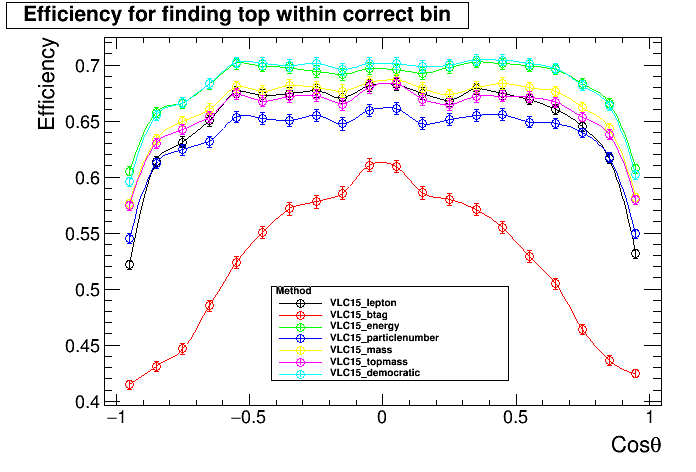
\includegraphics[width=0.6\textwidth]{figures/EfficiencyvsMCTheta.png}
  \caption[Efficiency for reconstructing the hadronically decaying top in the correct Cos$\theta$ bin]{Efficiency for reconstructing the hadronically decaying top in the correct Cos$\theta$ bin}
  \label{fig:angularEfficiency}
\end{figure}








\subsection{S' Reconstruction}

\begin{figure}
  \centering
  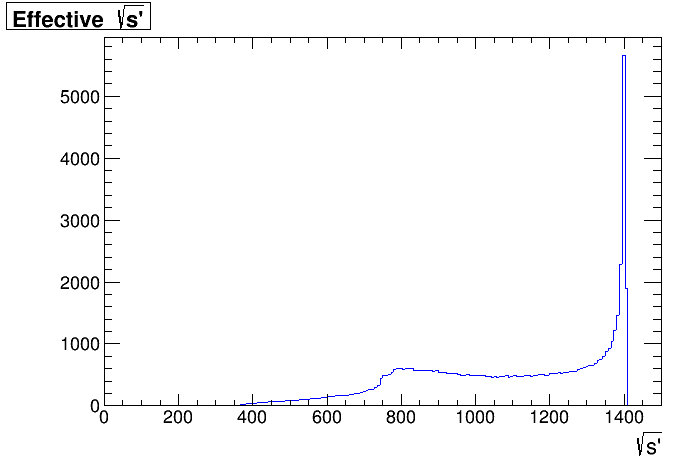
\includegraphics[width=0.6\textwidth]{figures/RawSPrime.png}
  \caption[Expected s' spectrum for $t\bar{t}$ at 1.4~TeV]{Expected s' spectrum for $t\bar{t}$ at 1.4~TeV}
  \label{fig:trueSPrime}
\end{figure}

Following the reconstruction of the lepton and hadronically decaying top it is already possible to calculate $A_{FB}^{t}$, however there is still benefit to first reconstructing the effective centre-of-mass energy of the events (along with the neutrino and any photons produced too.) This allows the calculation of $A_{FB}^{t}$ to be determined in the $t\bar{t}$ rest frame where it is predicted to be up to 50\% bigger \cite{Krohn:2011tw}, and also allows a differential measurement of $A_{FB}^{t}$ to be performed. The expected $\sqrt{s'}$ spectrum for $t\bar{t}$ production at 1.4~TeV is shown in figure \ref{fig:trueSPrime}. Here it is seen that there is a large tail to the energy spectrum which can be taken advantage of to measure $A_{FB}^{t}$ over a large range of energies. This differential measurement provides more greater power for discriminating between different phyhsics models than a single $A_{FB}^{t}$ measurement. If s' can not be reconstructed per event, $A_{FB}^{t}$ would have to either be measured as an integral over the full s' range or be measured just around the peak energy where there are only small s' corrections (E>1200~GeV), however this would mean disregarding INSERT PERCENTAGE of events produced during the 1.4~TeV run. As well as directly effecting the ways in which we can measure $A_{FB}^{t}$, reconstructing s' typically involves reconstructing the neutrino and photon contributions in the event. Having the information about these objects provides further information that can be used to reconstruct the leptonic top and help distinguish signal events from similar backgrounds.

In order to reconstruct s', multiple methods were attempted with varying complexity:

\subsubsection{Transverse/Longitudinal Association}
The simplest method attempted was to assume that all missing momentum in the transverse direction is attributed to the neutrino, while all longitudinal momentum comes from photon contributions. These assumptions are motivated by the results from figure \ref{fig:photonspectrum} which show that the photons produced are predominantly collinear with the beam.

\begin{figure}
  \centering
  
\includegraphics[width=0.6\textwidth]{figures/dummy}
  \caption[Angular energy distribution of initial state photons]{Angular energy distribution of initial state photons}
  \label{fig:photonspectrum}
\end{figure}

This allows full reconstruction of the neutrino and photon objects and so s' can be reconstructed by looking at the sum of the energy of the reocnstructed objects (excluding the photon as it is from ISR or Beamstrahlung.) A comparison of the reconstructed s' to the true s' spectrum is shown in figure \ref{fig:simpleAssoication}

\begin{figure}
  \centering
  
\includegraphics[width=0.6\textwidth]{figures/dummy}
  \caption[Reconstructed s' vs true s' for Transverse/Longitudinal Association Method]{Reconstructed s' vs true s' for Transverse/Longitudinal Association Method}
  \label{fig:simpleAssoication}
\end{figure}

\subsubsection{Analytic Mass Constraint}

\begin{figure}
  \centering
  
\includegraphics[width=0.6\textwidth]{figures/dummy}
  \caption[Reconstructed s' vs true s' for mass constraint method]{Reconstructed s' vs true s' for mass constraint method}
  \label{fig:MassConstraint}
\end{figure}

\begin{figure}
  \centering
  
\includegraphics[width=0.6\textwidth]{figures/dummy}
  \caption[Mass of reconstructed top when using mass constraint method]{Mass of reconstructed top when using mass constraint method}
  \label{fig:TopMassFrommassMethod}
\end{figure}

The second method attempted is an adaptation of the first method that makes use of the high efficiency with which the lepton is reconstructed to improve the performance. It starts in the same manor by assuming that all transverse missing momentum comes from the neutrino, however the missing longitudinal momentum is then divided beween the neutrino and photon. This is done by constraining the z component of the neutrino momentum by insisting the combination of the lepton and neutrino four momenta reproduces the W mass. The details of the necessary calculations are described in more detail in (PUT AN APPENDIX IN), but the key detail is that there are four possible solutions for the neutrino momentum. To decide the most suitable solution the W is combined with the b jet and the solution found to give an invaraint mass closest to the top mass was chosen to be best. The resulting reconstructed top mass and s' reconstruction performance are shown in figures \ref{fig:MassConstraint} and \ref{fig:TopMassFrommassMethod}.The reconstructed s' is seen to agree well with the true value for energies over \~900~GeV, however below this the performance is considerably worse.

\subsubsection{Collinearity}

\begin{figure}
  \centering
  
\includegraphics[width=0.6\textwidth]{figures/dummy}
  \caption[Collinearity of $t\bar{t}$ pair]{Collinearity of $t\bar{t}$ pair}
  \label{fig:Collinearity}
\end{figure}

\begin{figure}
  \centering
  
\includegraphics[width=0.6\textwidth]{figures/dummy}
  \caption[Reconstructed s' vs true s' for collinearity method]{Reconstructed s' vs true s' for collinearity method}
  \label{fig:CollinearitySPrime}
\end{figure}

\subsubsection{Kinematic Fitting}







\subsection{Flavour Tagging}
\label{Flavour Tagging}

\begin{figure}[t]
  \centering
  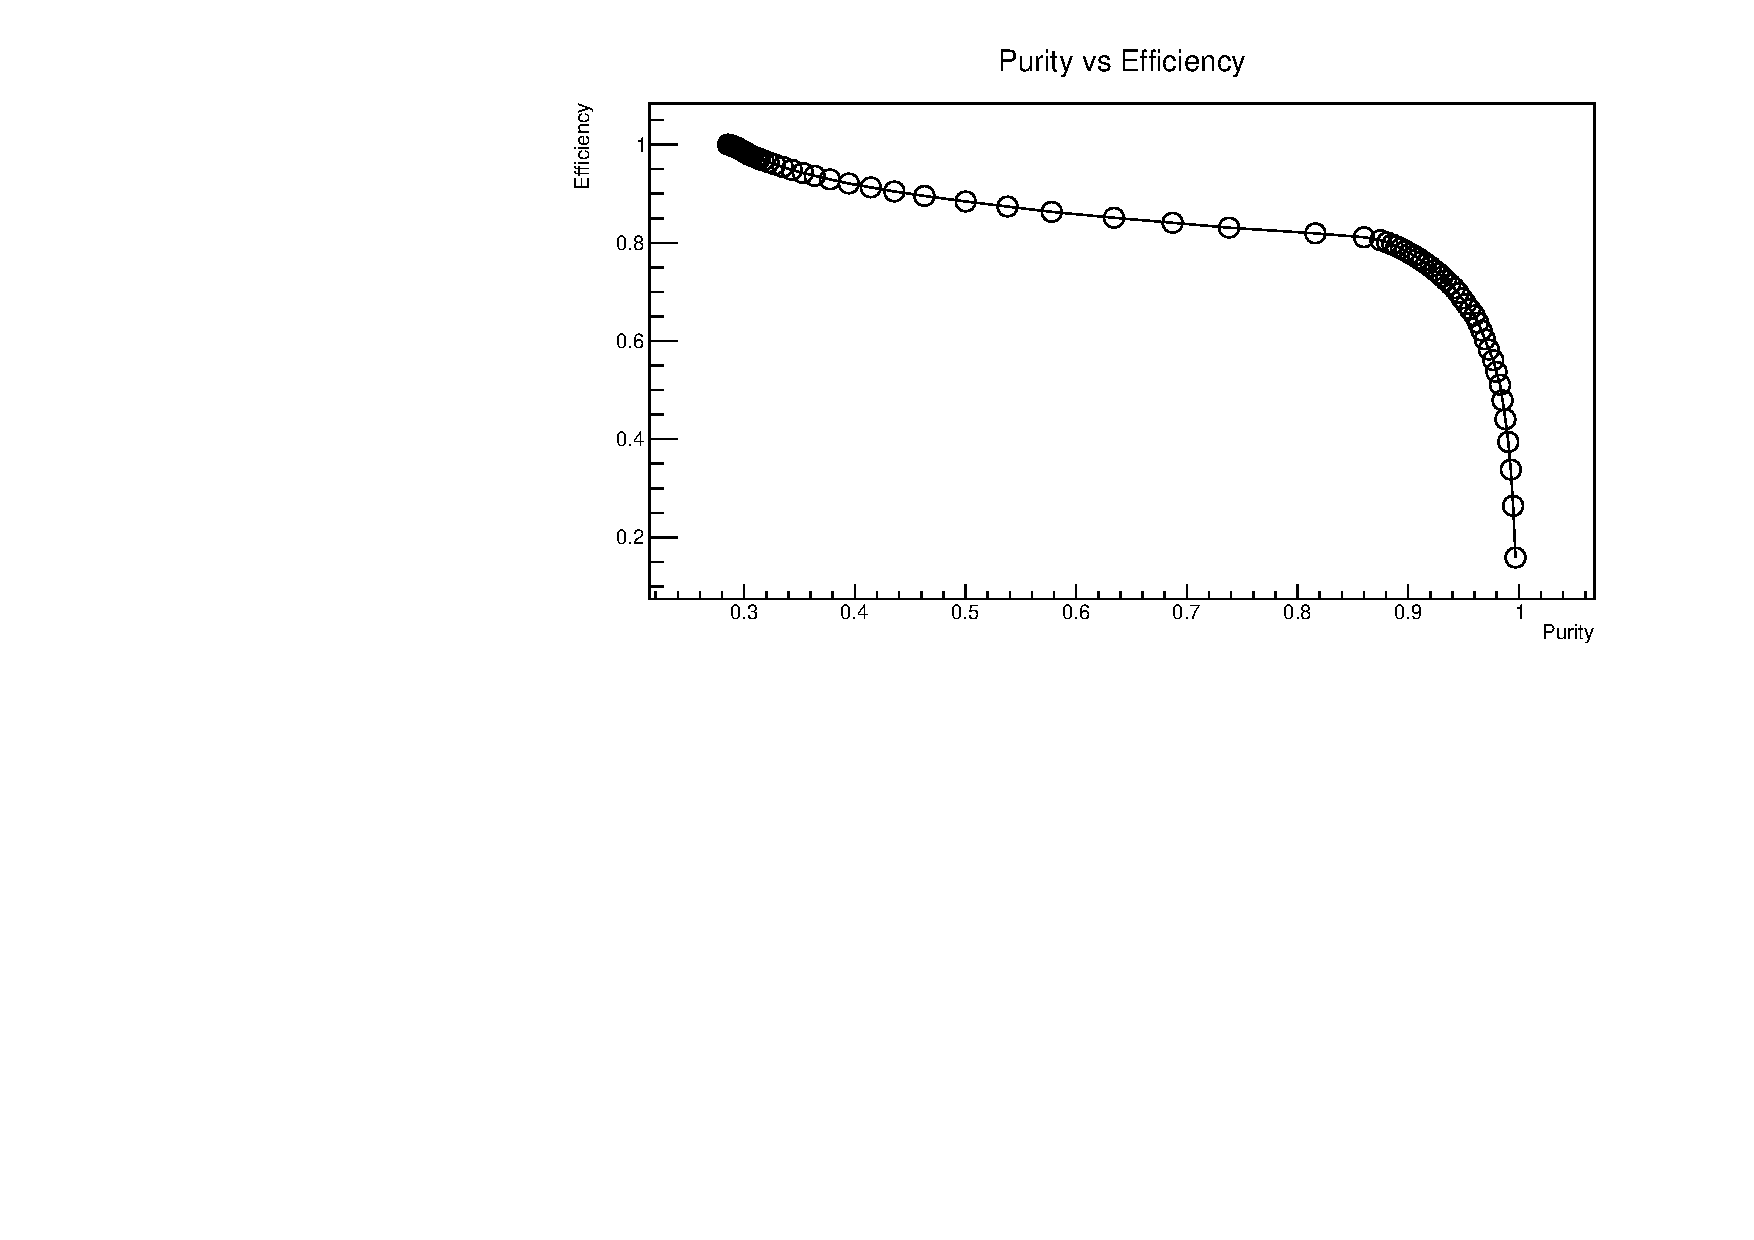
\includegraphics[width=0.78\textwidth,height=7cm,keepaspectratio]{figures/btag_crosses}
  \caption[B-Tagging Purity vs Efficiency]{Purity vs efficiency for identifying b-jets, obtained from a sample of Z$\rightarrow$ light, c and b quark events simulated at $\sqrt{s}=$1.4 TeV}
  \label{fig:Zbtagging}
\end{figure}


Flavour tagging was performed using LCFIPlus v00-05-02\cite{Suehara:2015ura}. LCFIPlus makes use of three BDTs dedicated to searching for u/d/s (light), b and c quarks respectively, to provide a b-tag and c-tag indicating the probability of a jet containing a b or c quark. As the signal process contains two b jets, only the results of the b-tag are considered here. The BDTs were trained using 50,000 $ee\rightarrow Z\nu\nu, Z\rightarrow qq$ events each. The base performance of the BDTs was assessed using a further 150,000 $ee\rightarrow Z\nu\nu, Z\rightarrow qq$ events containing an even mixture of bb, cc and light quarks to measure the efficiency and purity that could be obtained. The results of this test (shown in \ref{fig:Zbtagging}) indicate that in the case of Z$\rightarrow$qq events high efficiencies and puritys of \~85\% can be acieved simultaneously. Before we apply the flavour tagging to our analysis we first recluster our events into four jets to try and capture the bjets separately from the light quark jets. This is done within the LCFIPlus package which uses the Durham algorithm by default. Ideally the BDTs would also be retrained using top events rather than Z, however due to limited sample sizes this was not a realistic option. The performance of the btagging for semileptonic top events was evaluated by comparing the highest and second highest b-tags assigned to any of the four jets in signal events to those in backgrounds. The results of this comparison are seen in figure \ref{fig:btagging}. It is clear that the btagging is consistantly successful in finding the first b jet, but is less reliable for finding a second b jet. This is expected due to the toplogy of the event. The b jet produced by the leptonically decaying top should be well isolated from everything but the lepton which is identified and removed with high efficiency whereas the bjet from hadronically decaying top will be close to two other jets meaning the jet finder is less likely to accurately associate the PFOs in that region to the correct initial quark. As a result the b jet from the leptonic side should be consistently reconstructed and tagged whereas the the b jet on the hadronic side will be less consistent as the efficiency for reconstructing the jet correctly is much lower. Despite the poorer perfomrnace of the second highest b-tag, both variables provide clear potential as discriminating variables for removing background. 


\begin{figure}
  \centering
  \begin{subfigure}{.5\textwidth}
    \centering
    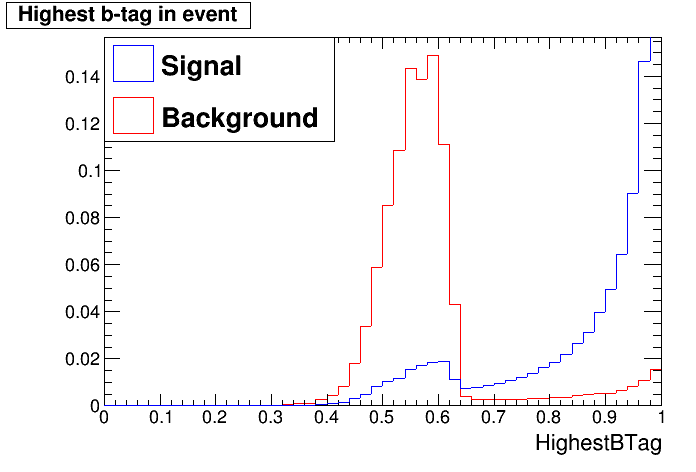
\includegraphics[width=0.9\textwidth]{figures/HighestBTag_SigVsBkg.png}
    \caption[Highest b-tag in event]{Highest b-tag in event}
  \end{subfigure}%
  \begin{subfigure}{.5\textwidth}
    \centering
    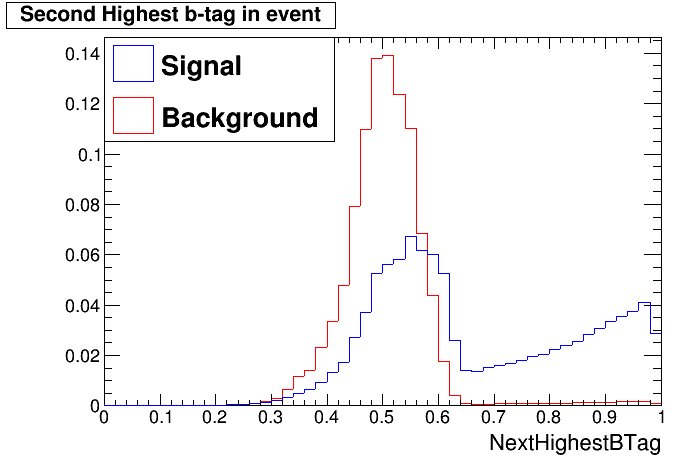
\includegraphics[width=0.9\textwidth]{figures/NextHighestBTag_SigVsBkg.png}
    \caption[Second Highest b-tag event in event]{Second Highest b-tag in event}
  \end{subfigure}
  \caption[B-Tagging performance]{B-Tagging performance}
  \label{fig:btagging}
\end{figure}




\section{Calculating AFB}
\label{Calculating AFB}

Measuring AFB from theta distributions vs counting- benefit that theta fit isn't effected by acceptance cutoff
Precision expected from just signal, no event selection, after preselection, after bdt
%Distribution with background included
%Distribution for signal + background with background subtraction
%Overall expected precision on Afb

\section{Event Selection}
\label{Event Selection}


Split into two regions- low and high energy due to different topology from s'

Using bdt based selection to maximise performance

Describe jet substructure variables (or any other confusing ones...)

\subsection{NSubjettiness}
\subsection{Subjet Angular Distributions}
\subsection{Jet Multiplicity}
\label{Jet Multiplicity}

\section{Quality Cuts}
\label{Quality Cuts}
Preselection cuts
BDT variables
Acceptance cuts

Large table showing efficiency of all cuts on all samples and the final expected number of events for full luminosity

Overall signal efficiency/purity/significance

\subsection{Differential Measurement}
Differential version of at least one of the plots- probably just signal before selection and then signal+background after selection with background subtraction.
Explain that most precise point will be for s' >1200 as there is the cleanest signal- highly boosted jets.
Suggest that lower s' results could benefit from a different reconstruction approach based on a resolved 4 jet analysis- probably deserves its own dedicated study though we can do if we have time. Would also likely benefit from having different variables used for the low s' BDT.


\section{Conclusions}

We measured the Afb to x precision....

\chapter{DECALStudies}


\chapter{Conclusion}

With the growing need to decide upon which future colliders should be built to ensure a smooth transition post LHC, it is vital that the relative merits of each proposed collider are examined. Here we have presented the potential impact that a lepton collider such as \ac{CLIC} can have on precision measurmements of the standard model. In the Higgs sector we have shown how the combination of several measurements can provide access to model independent measurements of the Higgs couplings, something not possible at hadron colliders. In particular we have shown how one of these measurements, $\sigma_{H\nu\bar{\nu}} \times BR(H\rightarrow WW^*)$, might be performed at 1.4 TeV using the semileptonic decay channel and collecting 1.5 ab$^{-1}$ of data. This yielded an expected precision of: \\[10pt]\centerline{\large{$\delta\sigma_{H\nu\nu}$ x BR(H$\rightarrow$WW$^*$) = 1.34\%$_{(Stat)} \oplus$ 1.37\%$_{(Syst)}$}} \\[10pt] Combining this with measurements performed with the fully hadronic channel shows an expected statistical precision of 1.0\%, typical of what can be expected for many measurements of Higgs properties at \ac{CLIC}.

\begin{table}[t]
  \centering
  \begin{tabular}{l|c|c}
    \toprule
    Energy (GeV) & $A_{FB}^t$ $\pm$ Stat. $\oplus$ Syst. & $\sigma$  $\pm$ Stat. $\oplus$ Syst.   \\
    \midrule
    \midrule
    \multicolumn{3}{l}{ P(e$^-$)=-80\%}\\
    \midrule
    $>=$1200   & 0.563 $\pm$ 0.018 $\oplus$ 0.015 & 18.41 $\pm$ 0.37 $\oplus$ 0.29\\
    \midrule
    900-1200   & 0.546 $\pm$ 0.034 $\oplus$ 0.028 & 11.01 $\pm$ 0.38 $\oplus$ 0.31\\
    \midrule
    400-900    & 0.458 $\pm$ 0.081 $\oplus$ 0.032 & 16.56 $\pm$ 1.31 $\oplus$ 0.48\\
    \midrule
    \midrule
    \multicolumn{3}{l}{ P(e$^-$)=+80\%}\\
    \midrule
    $>=$1200  & 0.621 $\pm$ 0.024 $\oplus$ 0.016 & 9.84 $\pm$ 0.28 $\oplus$ 0.14\\
    \midrule
    900-1200  & 0.588 $\pm$ 0.045 $\oplus$ 0.027 & 5.87 $\pm$ 0.29 $\oplus$ 0.14\\
    \midrule
    400-900   & 0.514 $\pm$ 0.105 $\oplus$ 0.034 & 8.63 $\pm$ 0.83 $\oplus$ 0.19\\
    \bottomrule
  \end{tabular}
  \caption{Final summary of the expected precisions attainable from the $t\bar{t}$ analysis.}
  \label{conlusiontable}
\end{table}

A study measuring the top forward backward asymmetry and $t\bar{t}$ cross section was also shown as a means of probing the ttX vertex for hints of \ac{BSM} physics contributions. This study was performed under the assumption that \ac{CLIC} would operate with an even luminsoity split between operation with an electron beam polarization of +80\% and -80\%. Due to the energy and polarization dependence of $A_{FB}^t$ and $\sigma_{t\bar{t}}$ and the presence of a large tail in the energy spectrum of collisions at \ac{CLIC}, the analysis was performed in six bins corresponding to the combinations of two polarization states and three energy ranges to maximise the information extracted. Event reconstruction and selection was performed using techniques based on fat jet and jet substructure which have not been implemented in a lepton collider before. Ultimately the final results were extracted by performing a second order polynomial fit to the distribution of the top production angle. The resulting uncertainties for each bin are shown in \reftab{conlusiontable} and are found to be approximately an order of magnitude better than what is seen at the \ac{LHC}\cite{Bai:2011uk}. A detailed study of various systematic effects revealed that the in all cases the uncertainty is dominated by the statistical component with the dominant systematic contributions for the cross section and $A_{FB}^t$ coming from the background normalization and bias introduced during efficiency corrections respectively. In future these results will be combined with measurements from other top studies performed by \ac{CLIC} to evaluate the precision to which the electroweak form factors of the ttX can be measured.

Lastly we have examined the possibility for using a \ac{DECAL} at the \ac{ILC} as an alternative to the analgue SiW calorimeter. Such a device would use \ac{CMOS} \ac{MAPS} technology to provide an ultra high granularity capable of measuring every particle present within an \ac{EM} shower providing potential benefits for use with particle flow techniques and potential cost reductions. The resolution of a \ac{DECAL} was found to be dominated by two competing effects. At low energy boundary crossings dominate leading to a worse performance for designs based on narrower, deeper pixels. For higher energy saturation occurs as the EM shower becomes denser than the detectors granularity leading to worse performance for wider pixels. When using DigiMAPS to apply additional levels of realism such as charge diffusion, dead space, noise, threshold spreads and clustering it was found that the clustering helped mitigate the impact of boundary crossings leading to a general performance for narrow pixels thin pixels. For the typical enegy scale of the \ac{ILC} the optimal piuxel desgin was found to occur when using 30 $\mu m$ pitch, 12 $\mu m$ epi thickness pixels. This design yielded an energy resolution of:

\begin{equation}
  \frac{\sigma_E}{E}=\frac{16.1\%}{\sqrt{E}} \oplus \frac{0.5\%}{E} \oplus 0.4\%
\end{equation}

Which is comparable to the performance seen for the fully optimised design of the analogue SiW intended for use in \ac{ILD}. 



%%%%%%%%%% Chapters %%%%%%%%%%

\setstretch{1}
\cleardoublepage
\renewcommand{\bibname}{REFERENCES}
\bibliographystyle{ieeetr}
\bibliography{thesis}

\cleardoublepage
\appendix
%%%%%%%%%% Appendix %%%%%%%%%%
\section{Appendix A: Higgs Results}
\label{appendixA}
Here we show the signal and background distributions for the input variables used for training the BDT for our Higgs analysis. In all cases the plots are normalised to unity and show the raw distributions before preselection cuts are applied.

\begin{figure}[h] 
  \begin{subfigure}[]{0.5\linewidth}
    \centering
    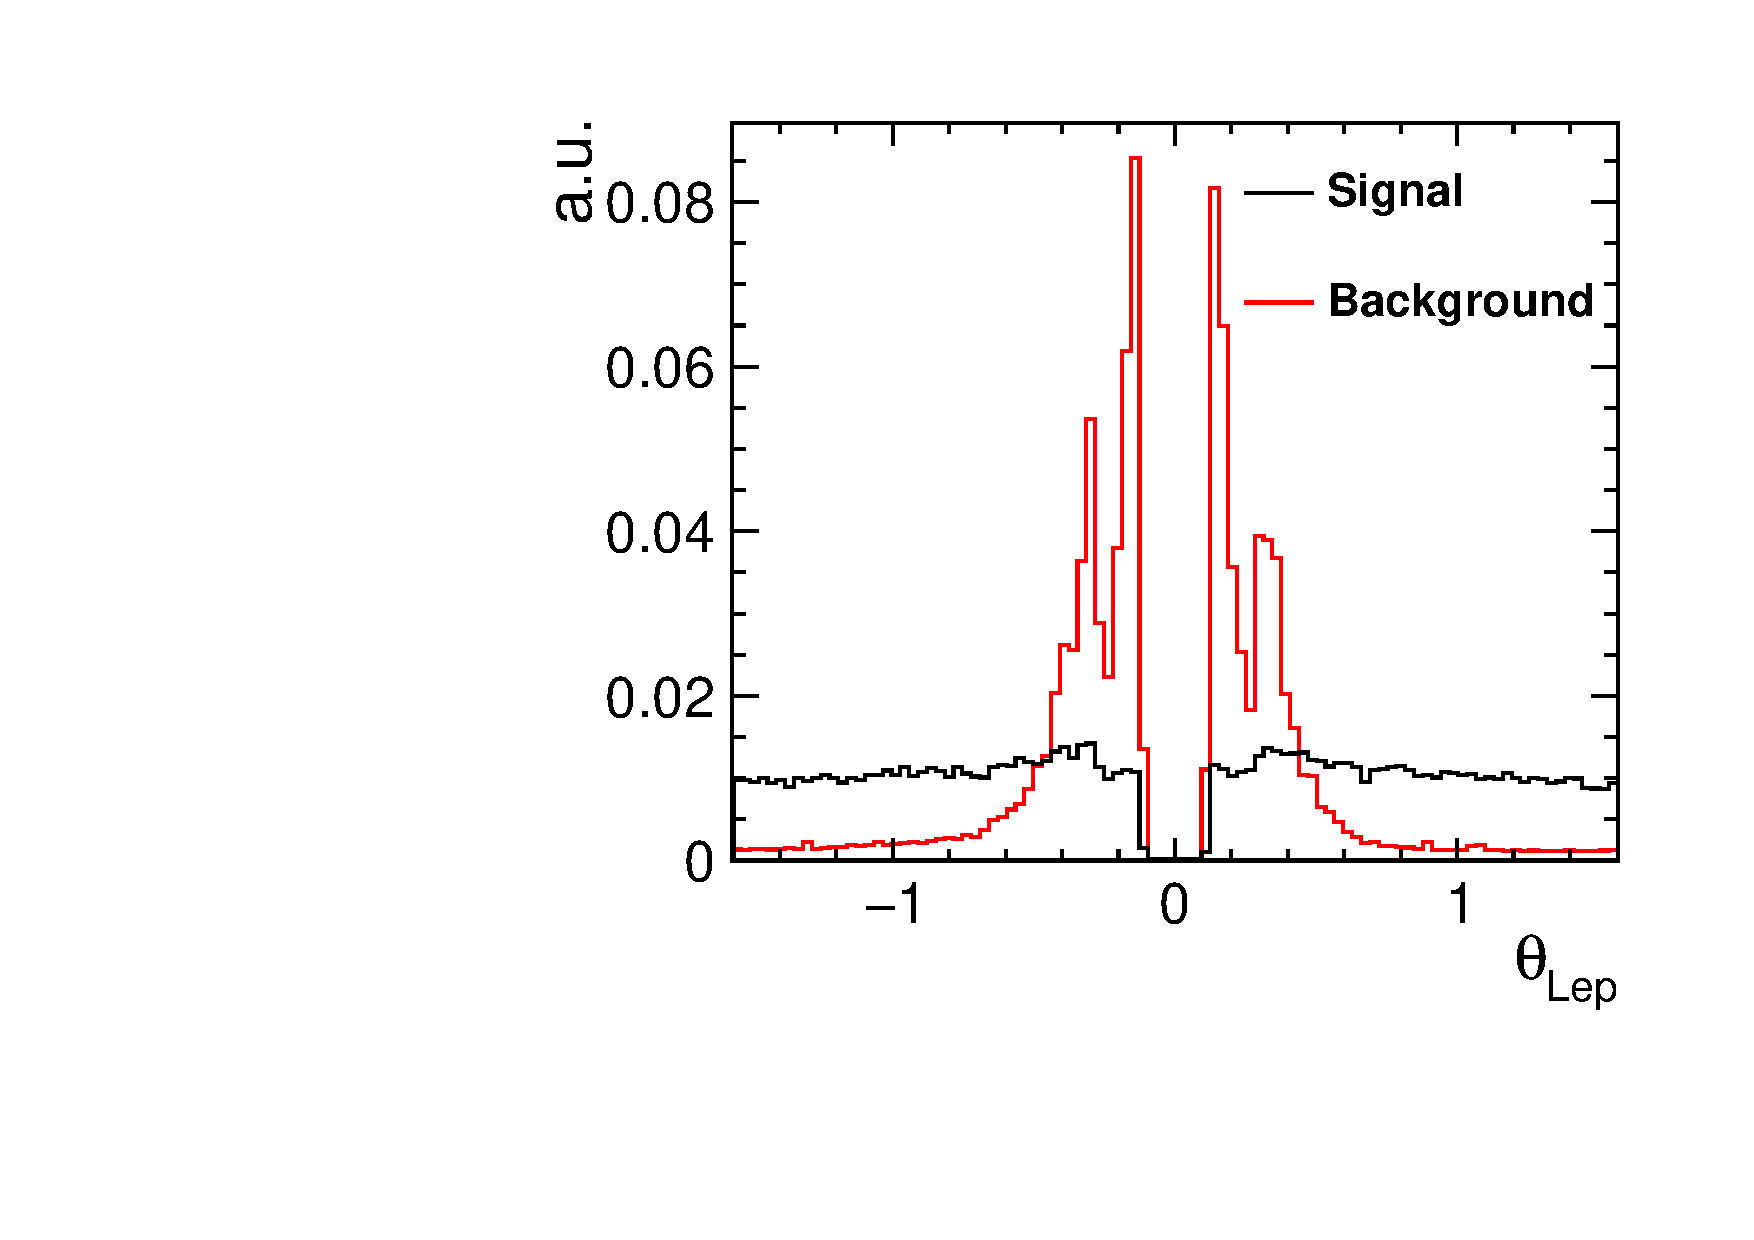
\includegraphics[width=0.75\linewidth]{Appendix/figures/DiraLep} 
    \caption{Angle of lepton relative to beam axis} 
    \vspace{4ex}
  \end{subfigure}%% 
  \begin{subfigure}[]{0.5\linewidth}
    \centering
    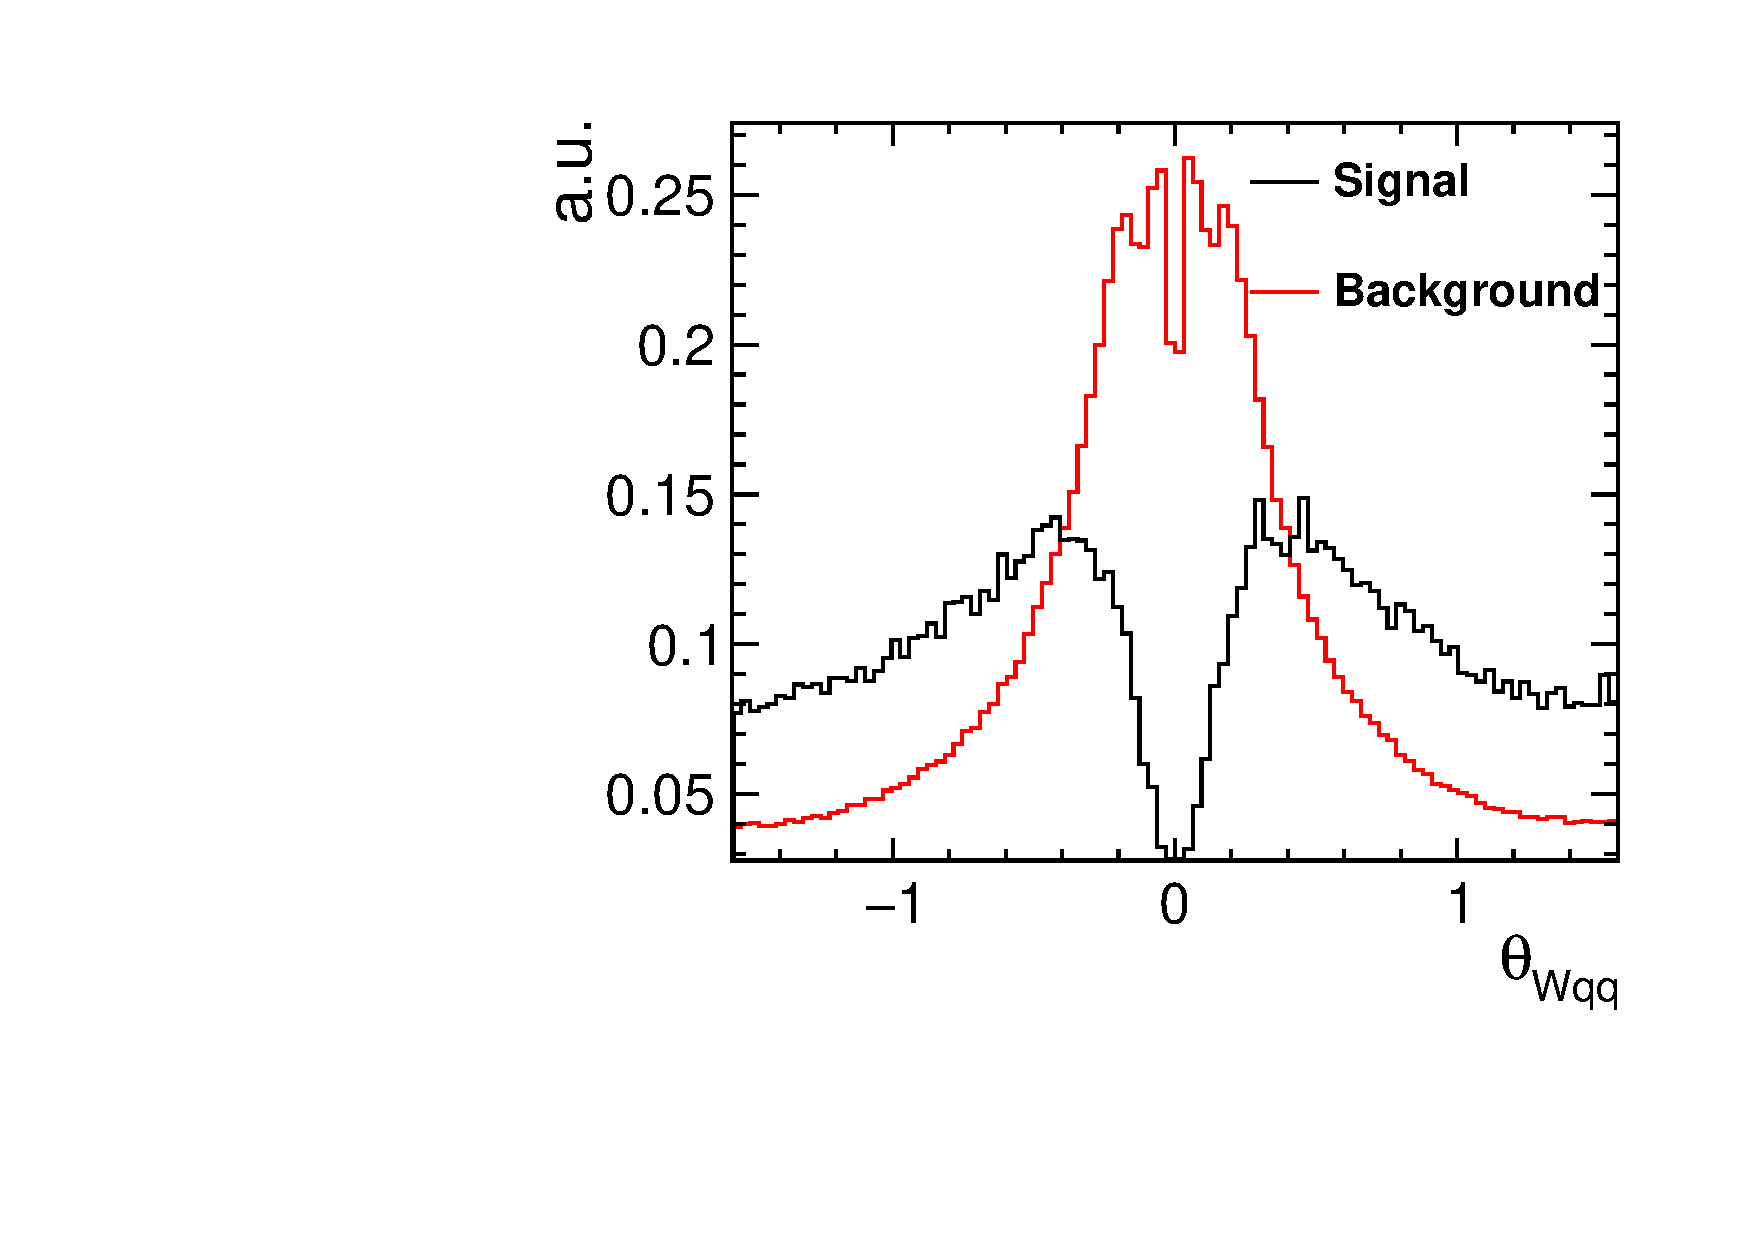
\includegraphics[width=0.75\linewidth]{Appendix/figures/DiraWqq} 
    \caption{Angle of W relative to beam axis} 
    \vspace{4ex}
  \end{subfigure}
    \begin{subfigure}[]{0.5\linewidth}
    \centering
    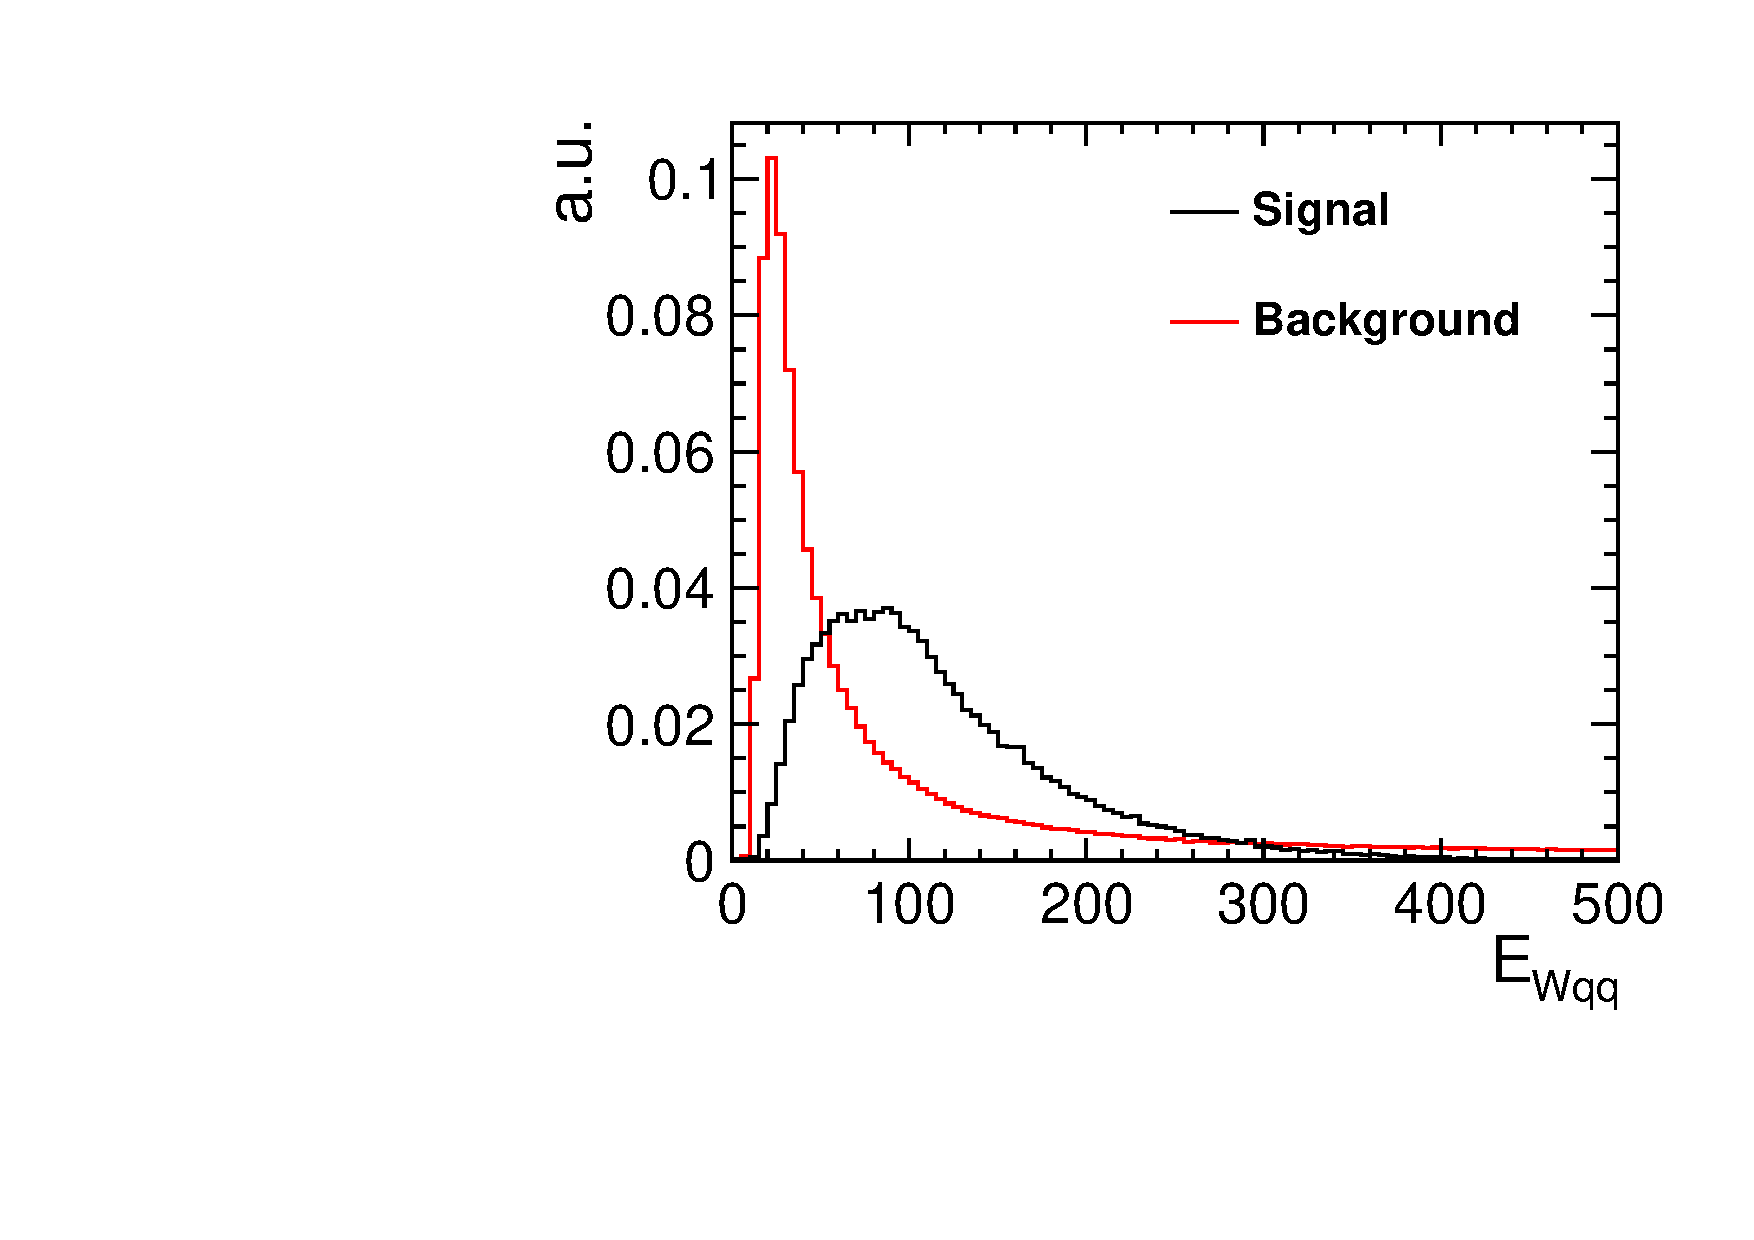
\includegraphics[width=0.75\linewidth]{Appendix/figures/EWqq} 
    \caption{Energy of hadronically decaying W} 
    \vspace{4ex}
  \end{subfigure}%% 
  \begin{subfigure}[]{0.5\linewidth}
    \centering
    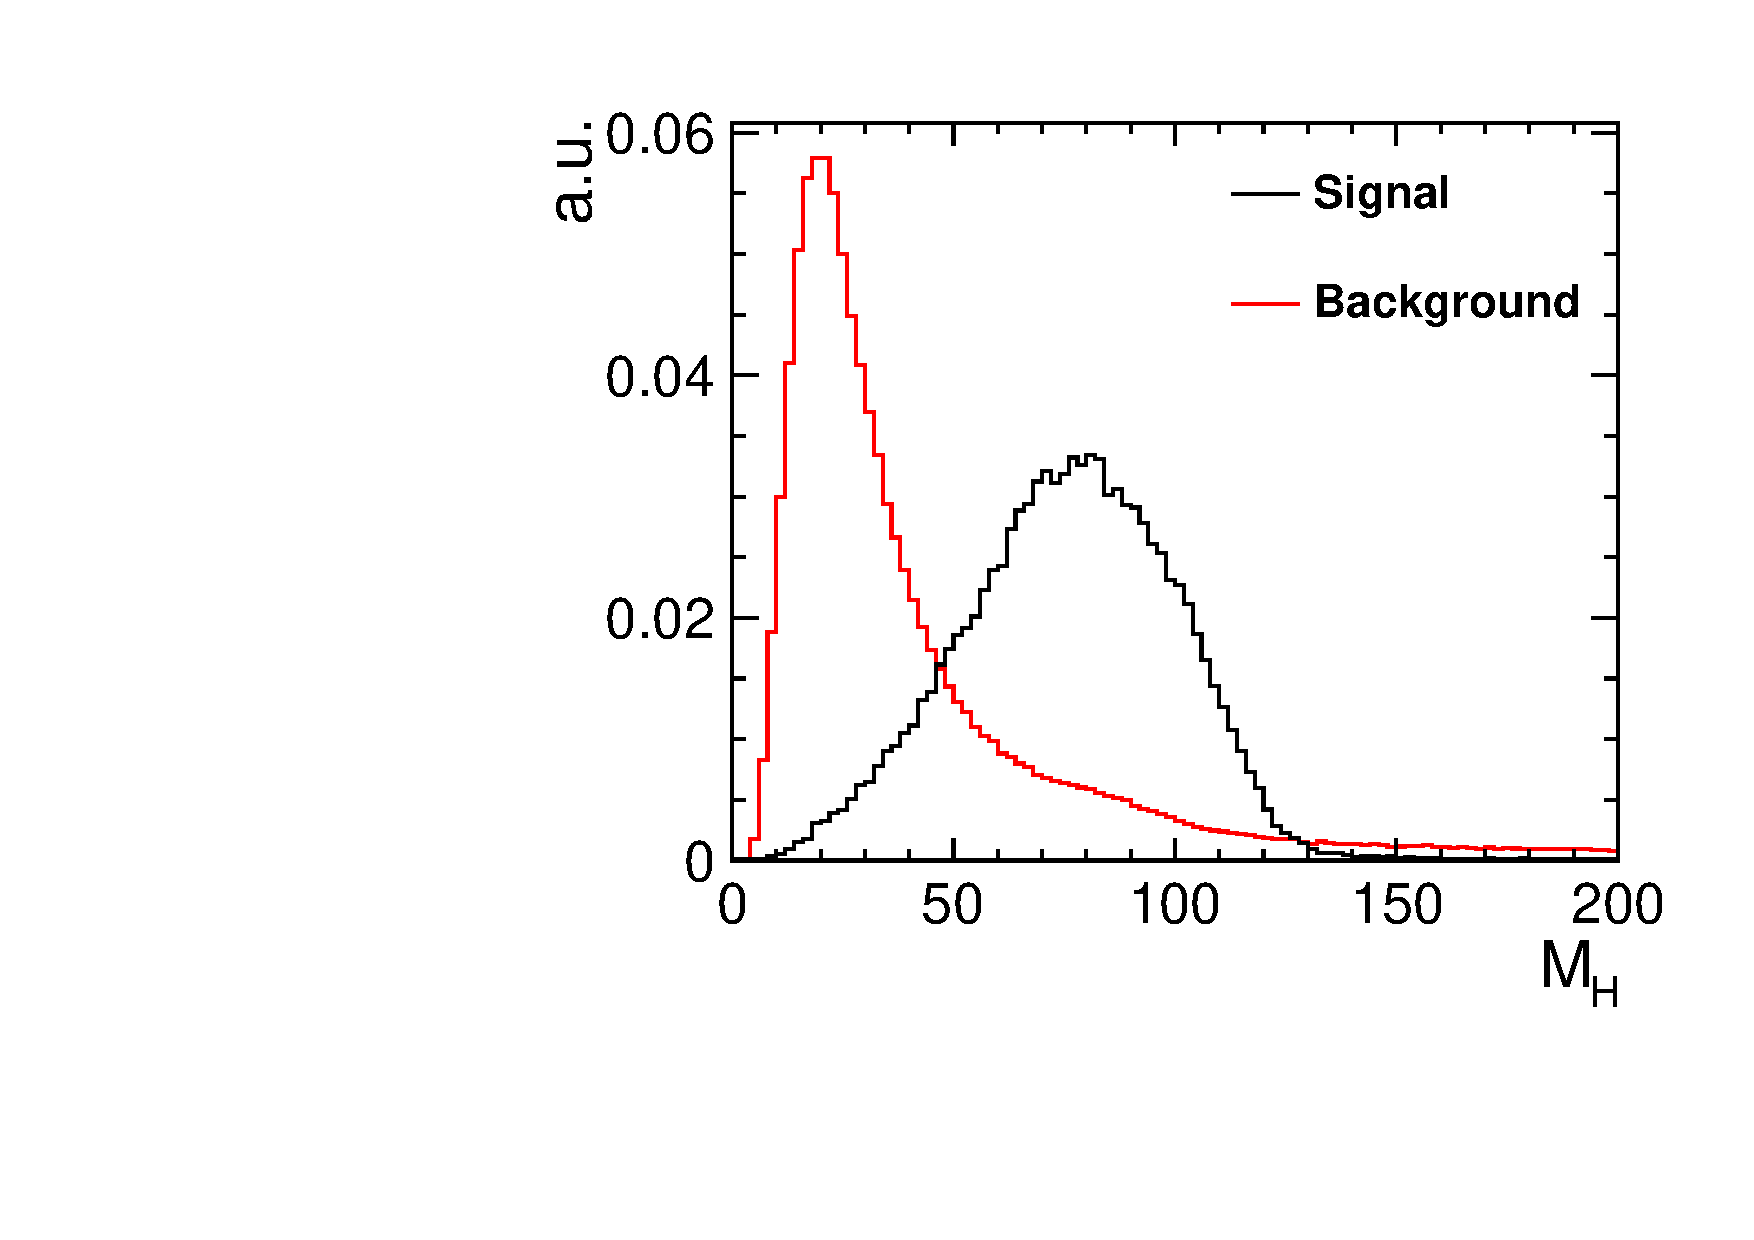
\includegraphics[width=0.75\linewidth]{Appendix/figures/HiggsMass} 
    \caption{Reconstructed Higgs mass} 
    \vspace{4ex}
  \end{subfigure}
    \begin{subfigure}[]{0.5\linewidth}
    \centering
    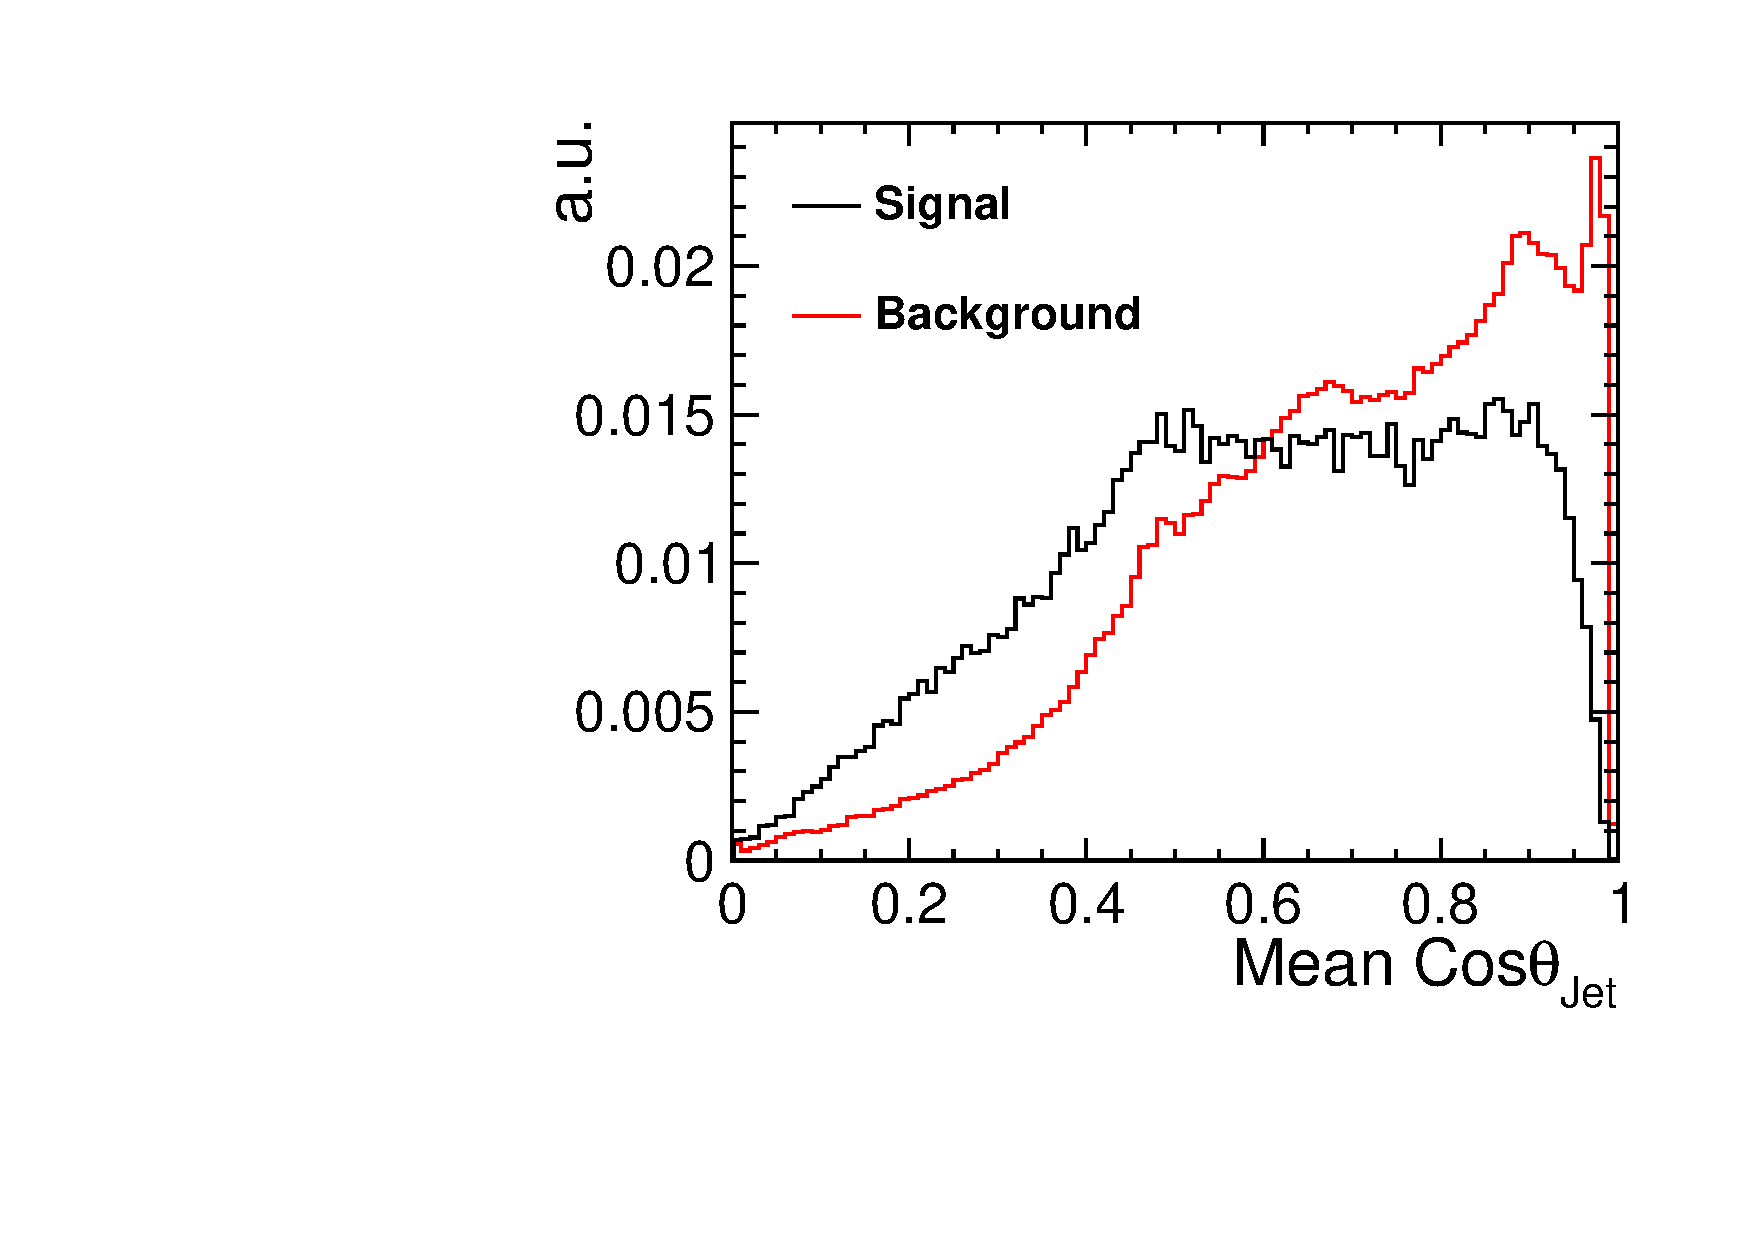
\includegraphics[width=0.75\linewidth]{Appendix/figures/JetCosTheta} 
    \caption{Average cos$\theta$ of jets} 
  \end{subfigure}%%
  \begin{subfigure}[]{0.5\linewidth}
    \centering
    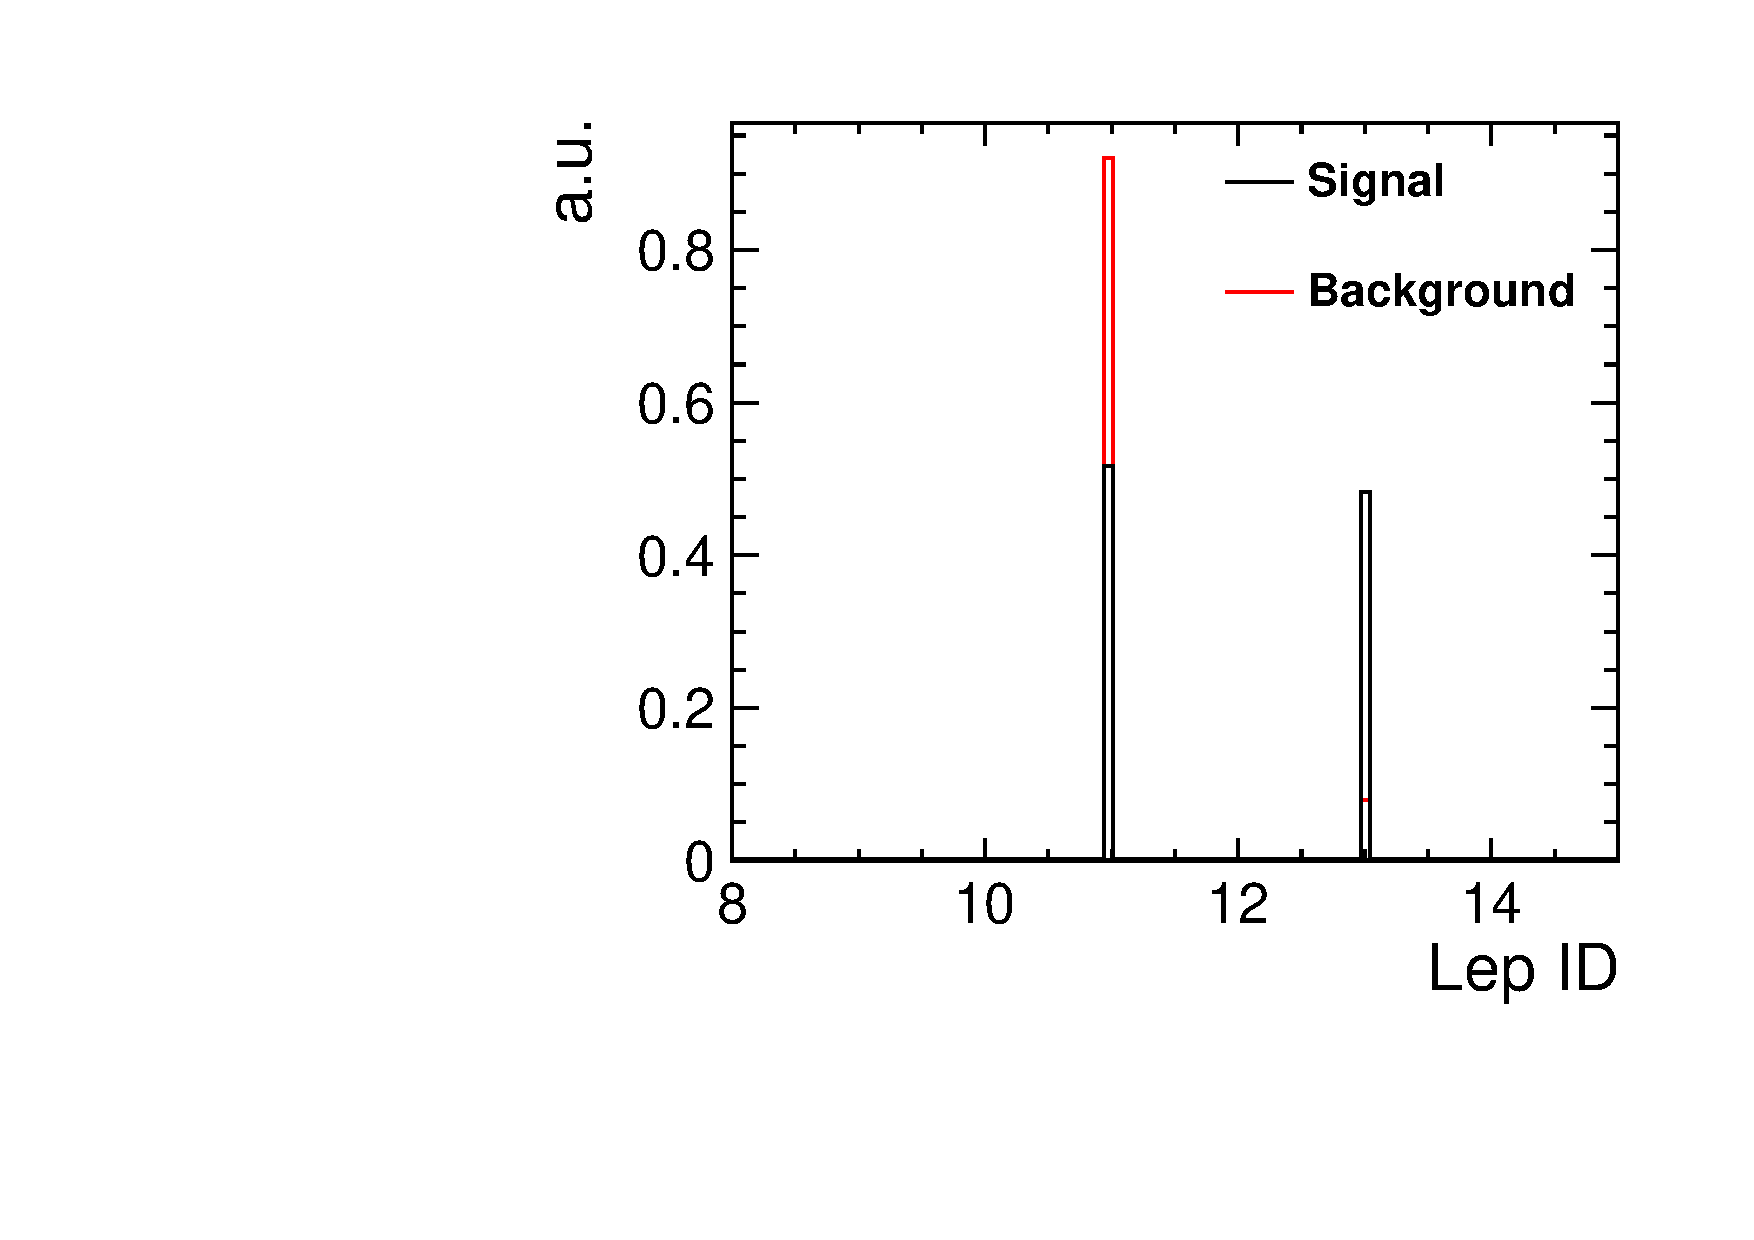
\includegraphics[width=0.75\linewidth]{Appendix/figures/LepID} 
    \caption{Lepton PID} 
  \end{subfigure}
\end{figure}


\begin{figure}[]\ContinuedFloat
    \begin{subfigure}[]{0.5\linewidth}
    \centering
    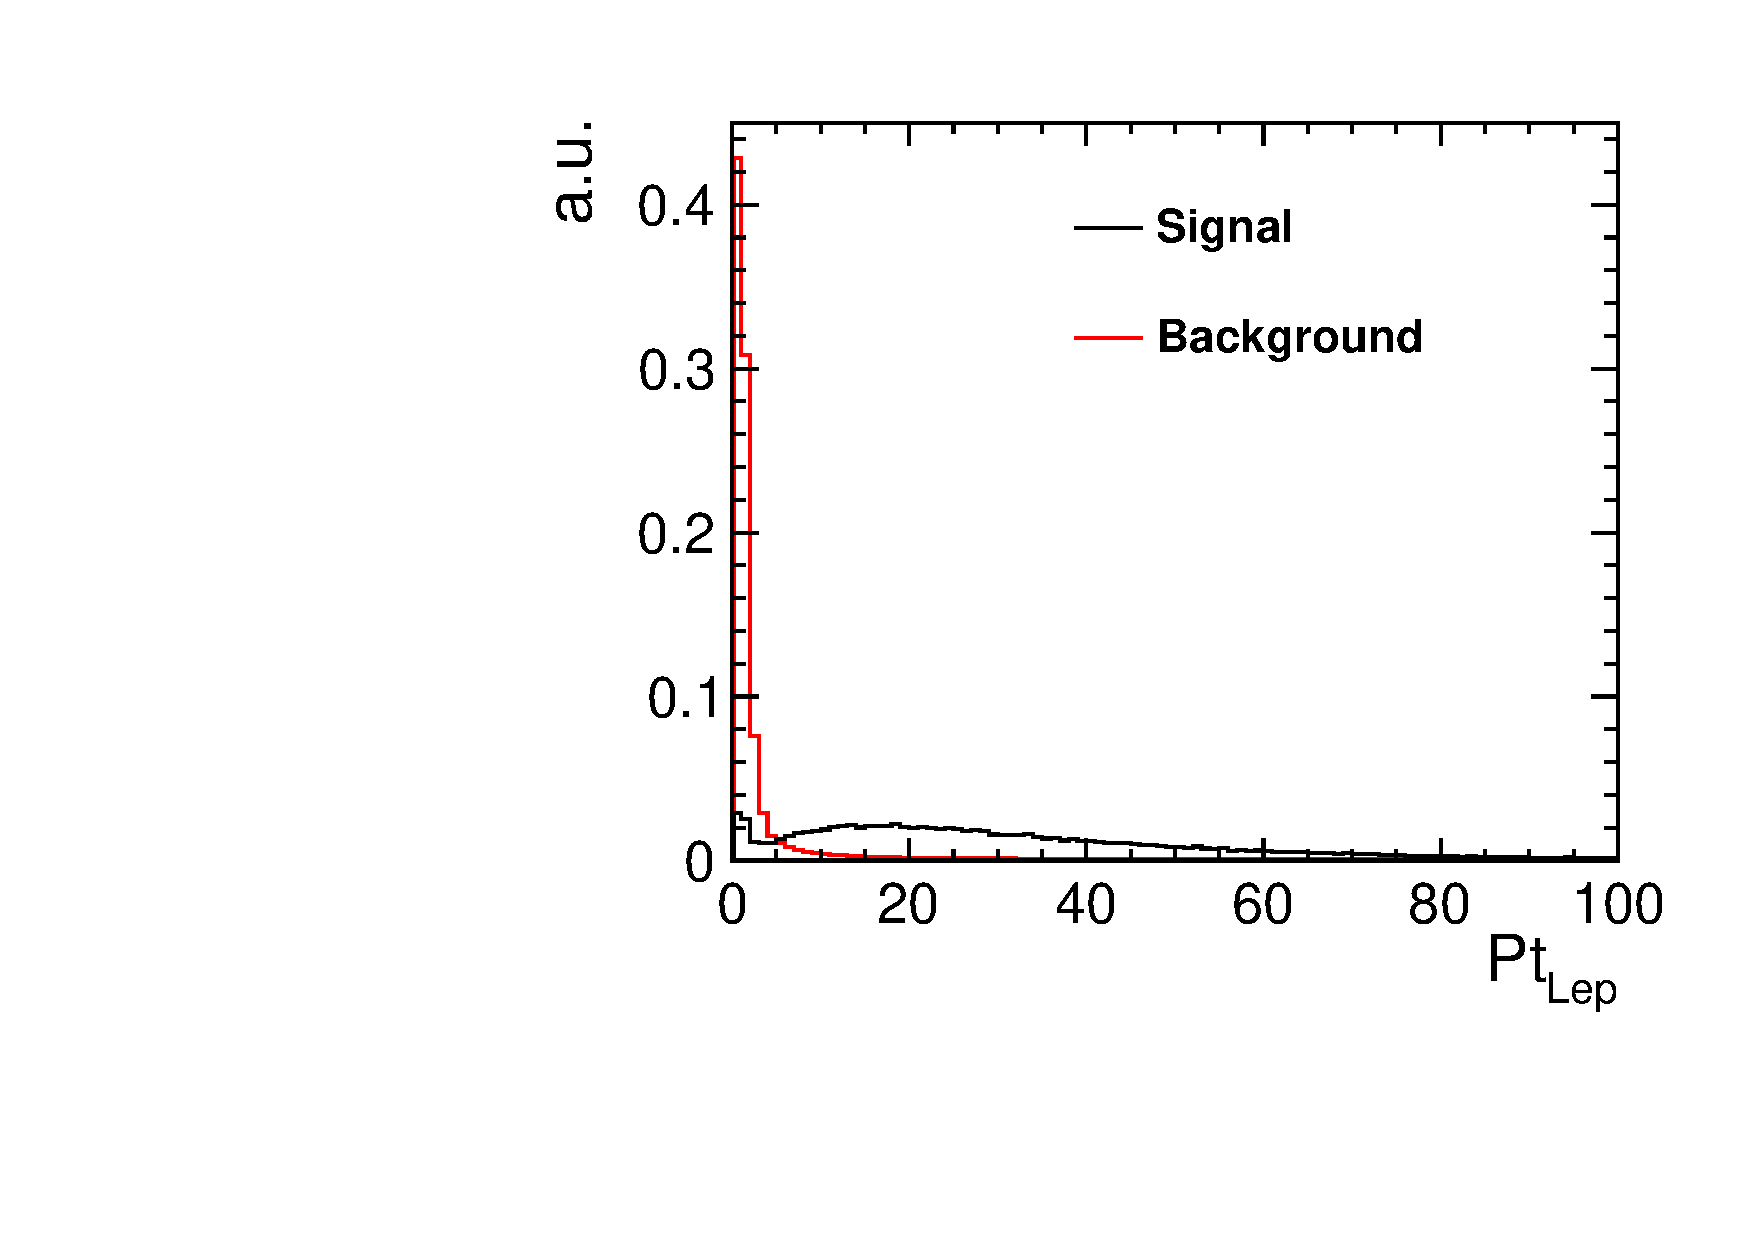
\includegraphics[width=0.75\linewidth]{Appendix/figures/LepPt} 
    \caption{Lepton Pt} 
  \end{subfigure}%%
  \begin{subfigure}[]{0.5\linewidth}
    \centering
    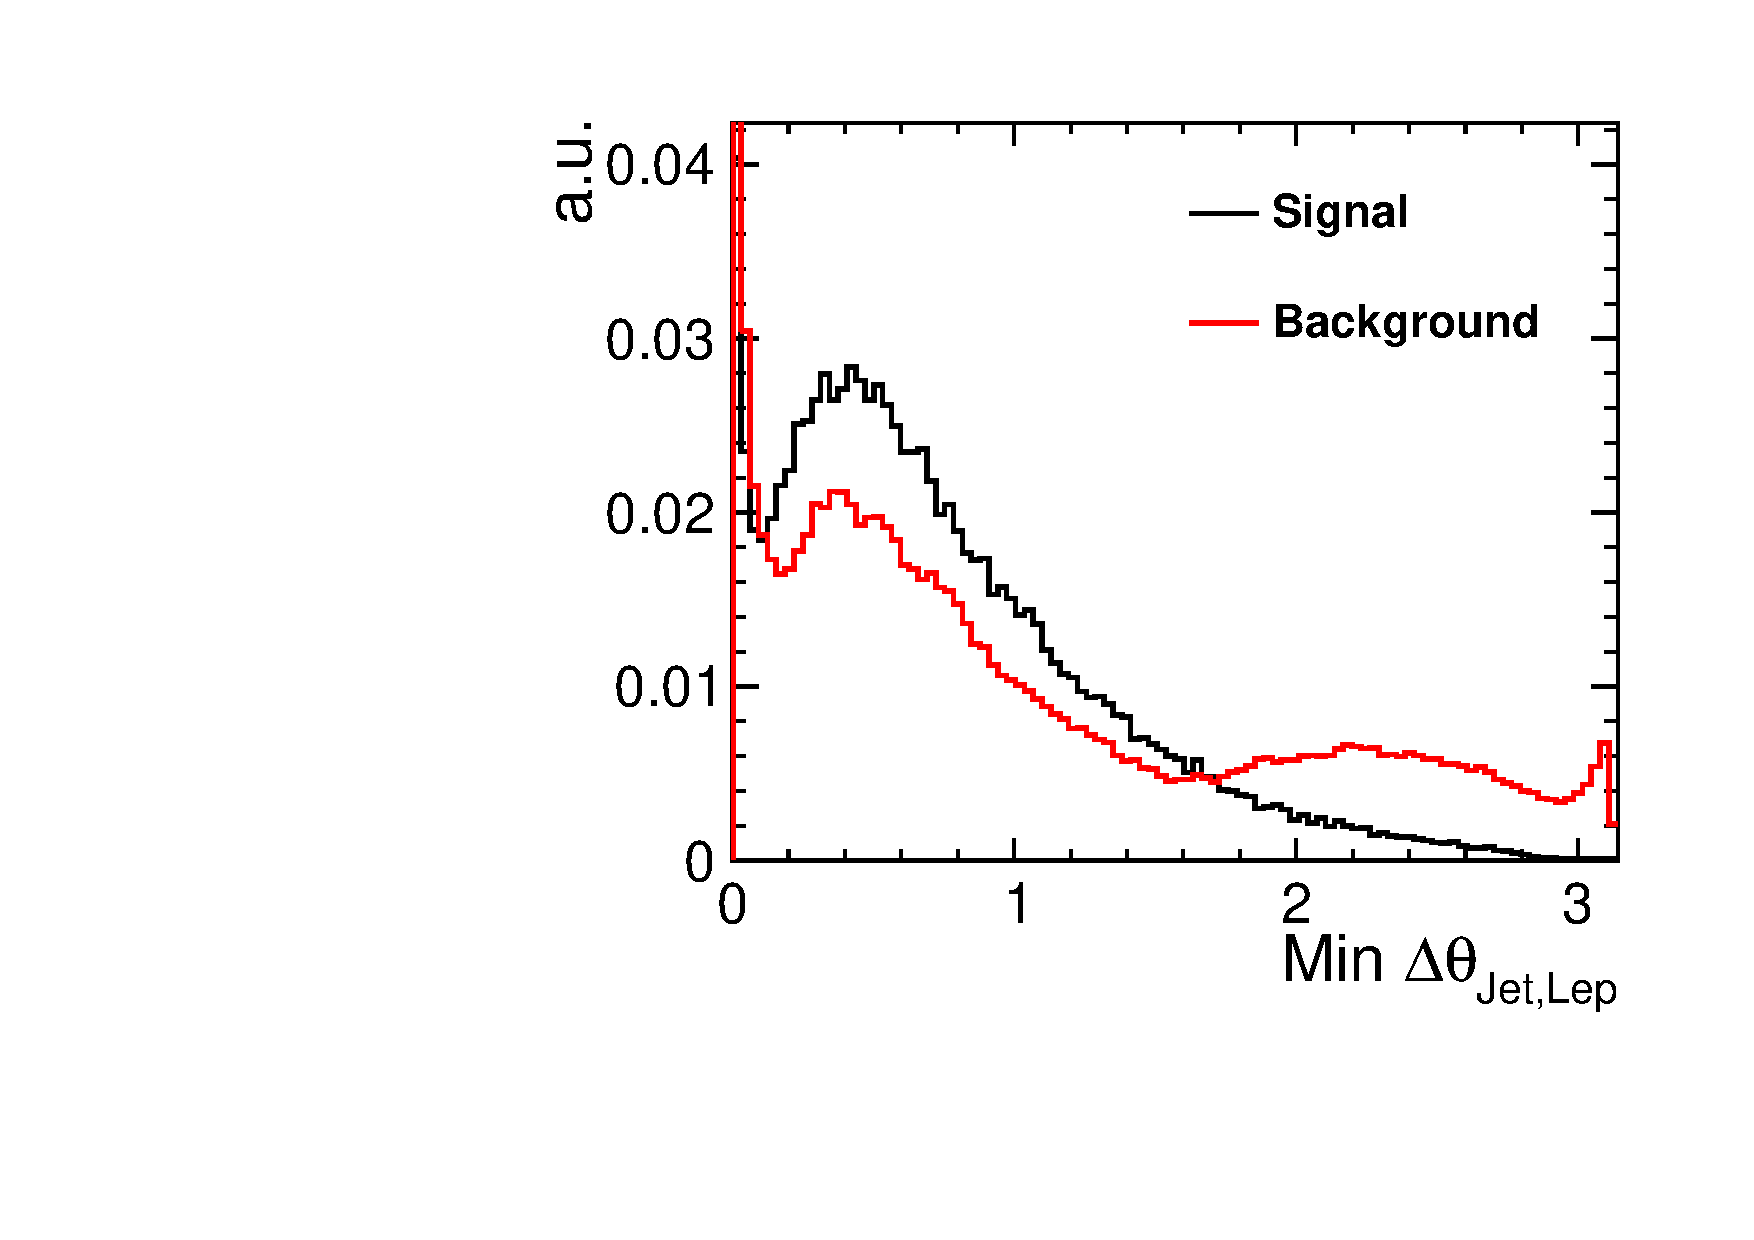
\includegraphics[width=0.75\linewidth]{Appendix/figures/MinJetLepAngSep} 
    \caption{Angular separation between lepton and nearest jet} 
  \end{subfigure}
  \begin{subfigure}[]{0.5\linewidth}
    \centering
    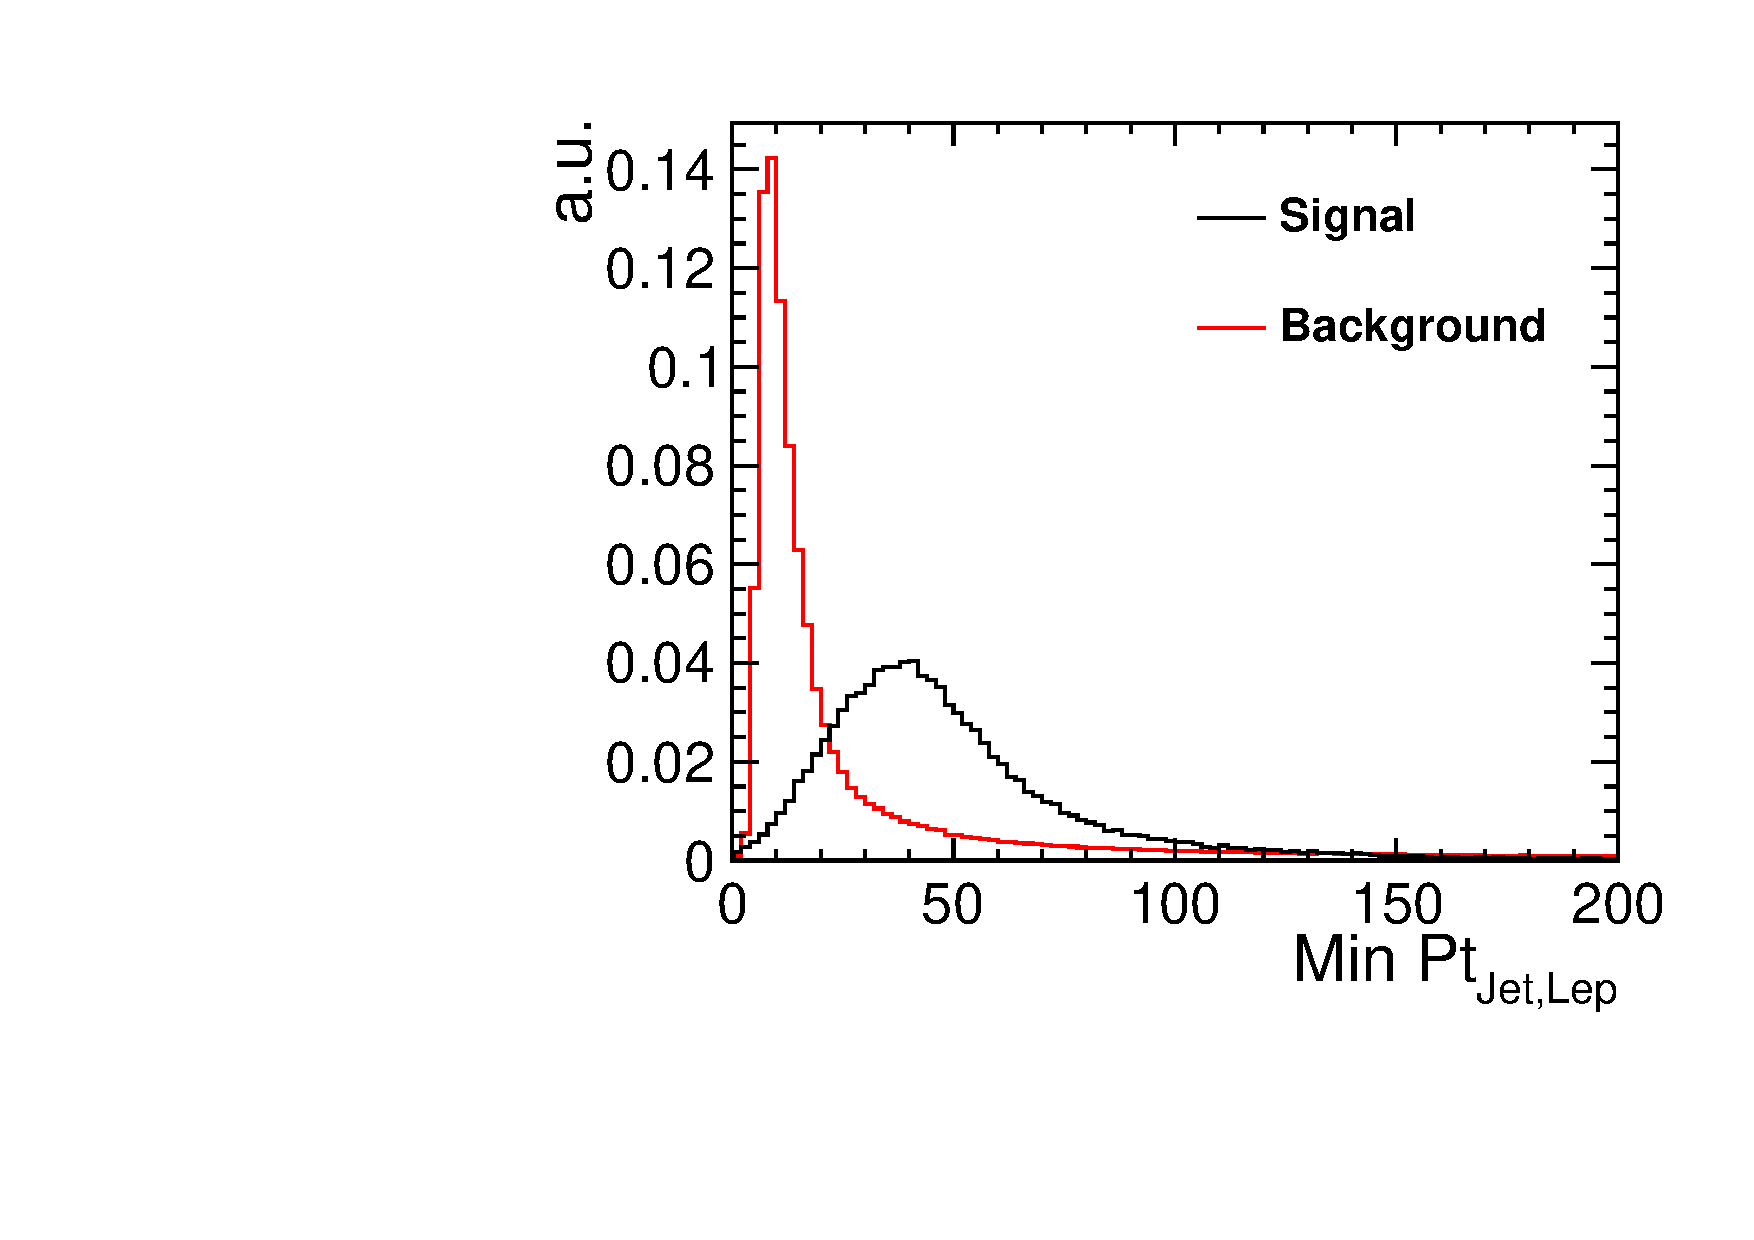
\includegraphics[width=0.75\linewidth]{Appendix/figures/MinJetLepPt} 
    \caption{Relative Pt between lepton and nearest jet} 
    \vspace{4ex}
  \end{subfigure}%% 
  \begin{subfigure}[]{0.5\linewidth}
    \centering
    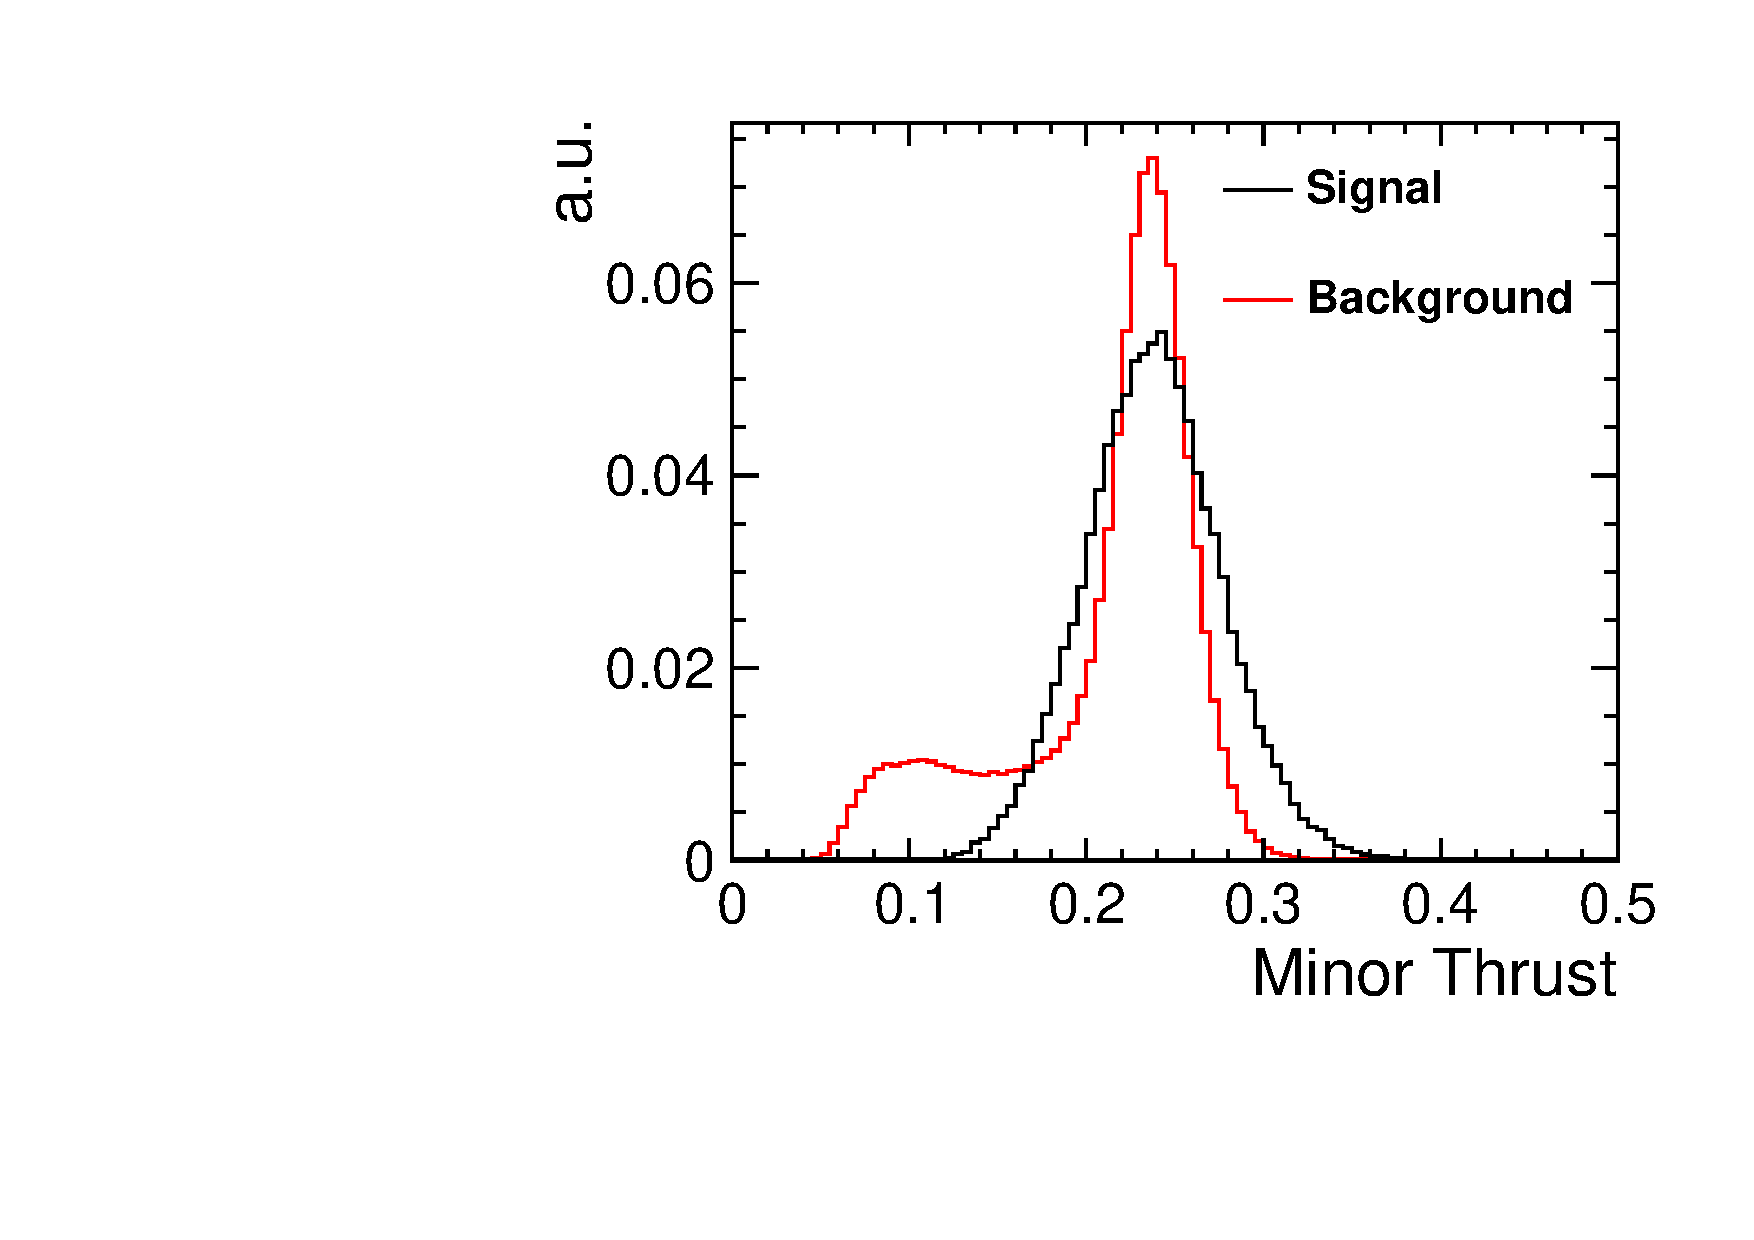
\includegraphics[width=0.75\linewidth]{Appendix/figures/MinorThrust} 
    \caption{Minor Thrust of the event} 
    \vspace{4ex}
  \end{subfigure} 
  \begin{subfigure}[]{0.5\linewidth}
    \centering
    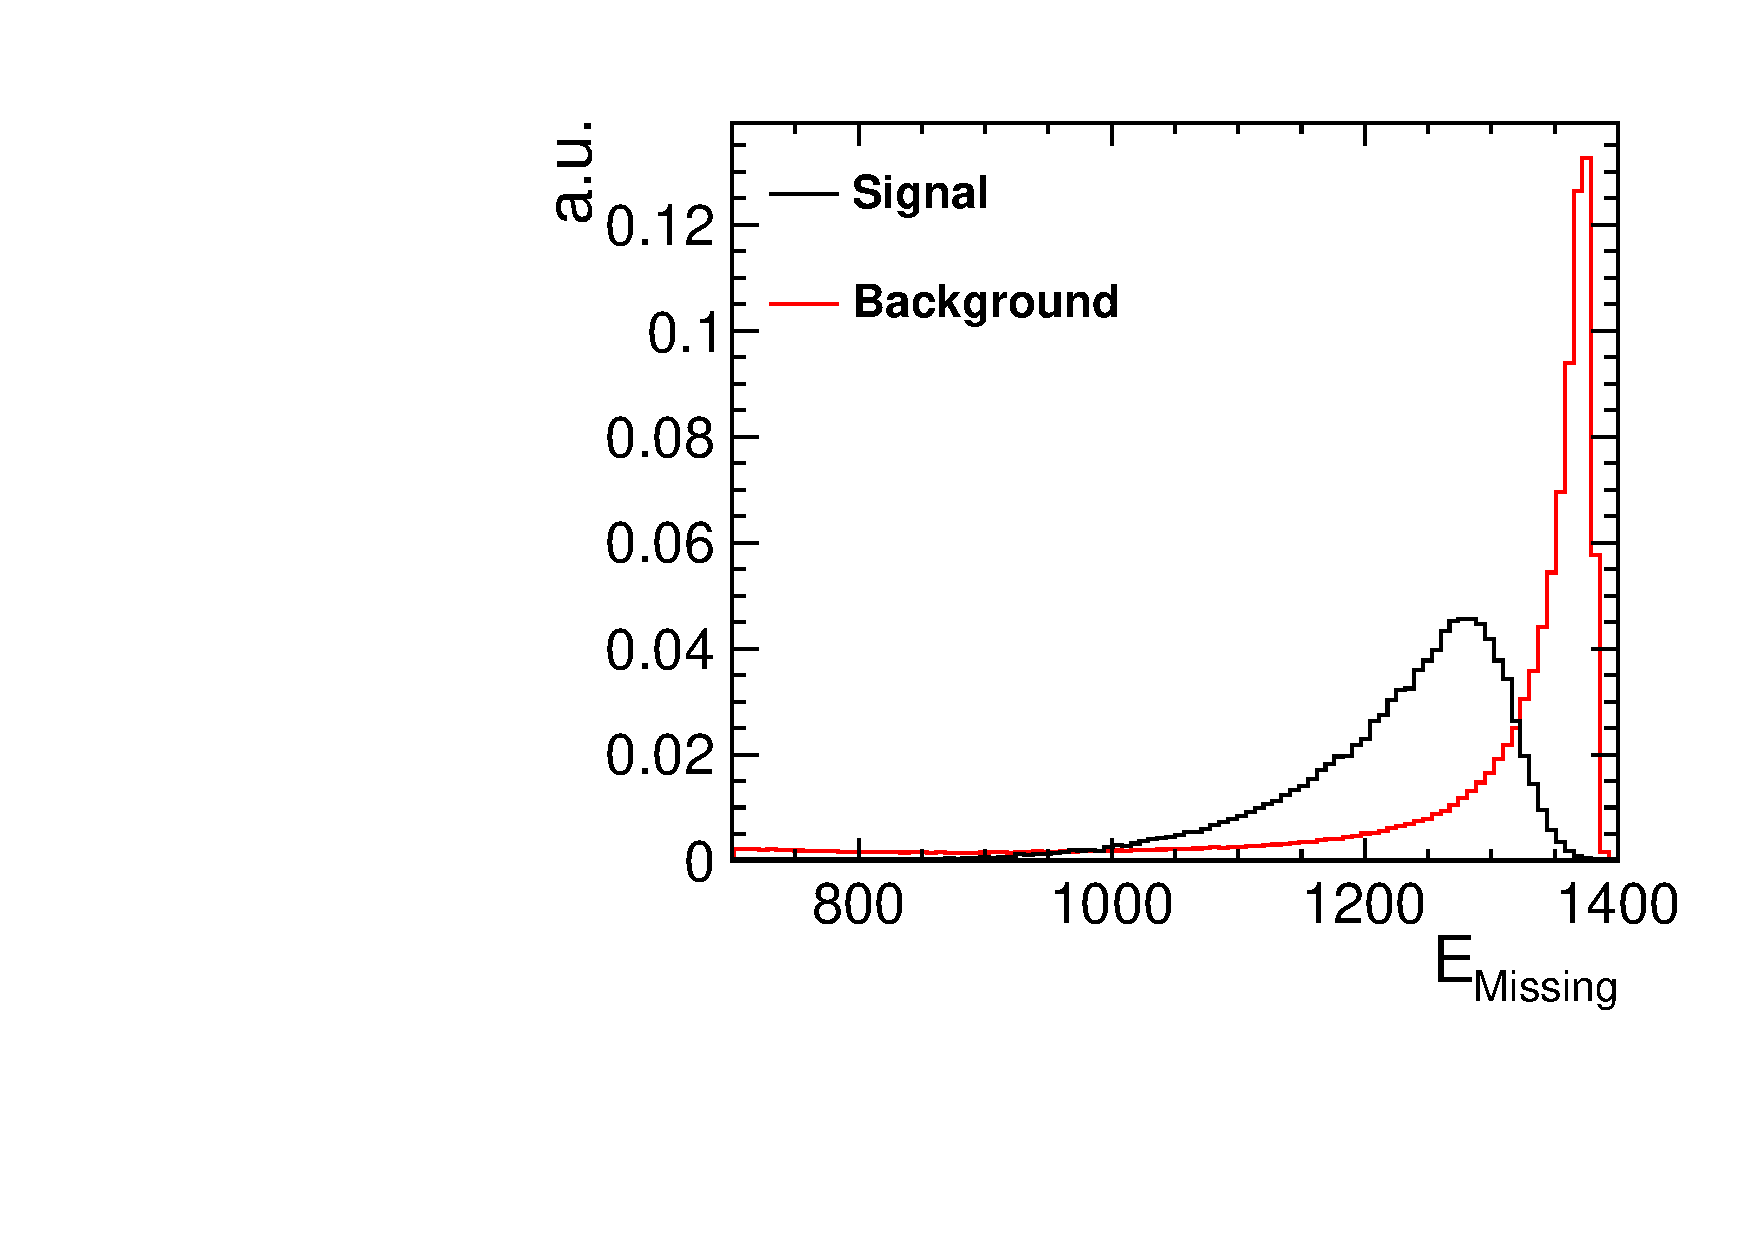
\includegraphics[width=0.75\linewidth]{Appendix/figures/MissingE} 
    \caption{Missing energy} 
    \vspace{4ex}
  \end{subfigure}%%
  \begin{subfigure}[]{0.5\linewidth}
    \centering
    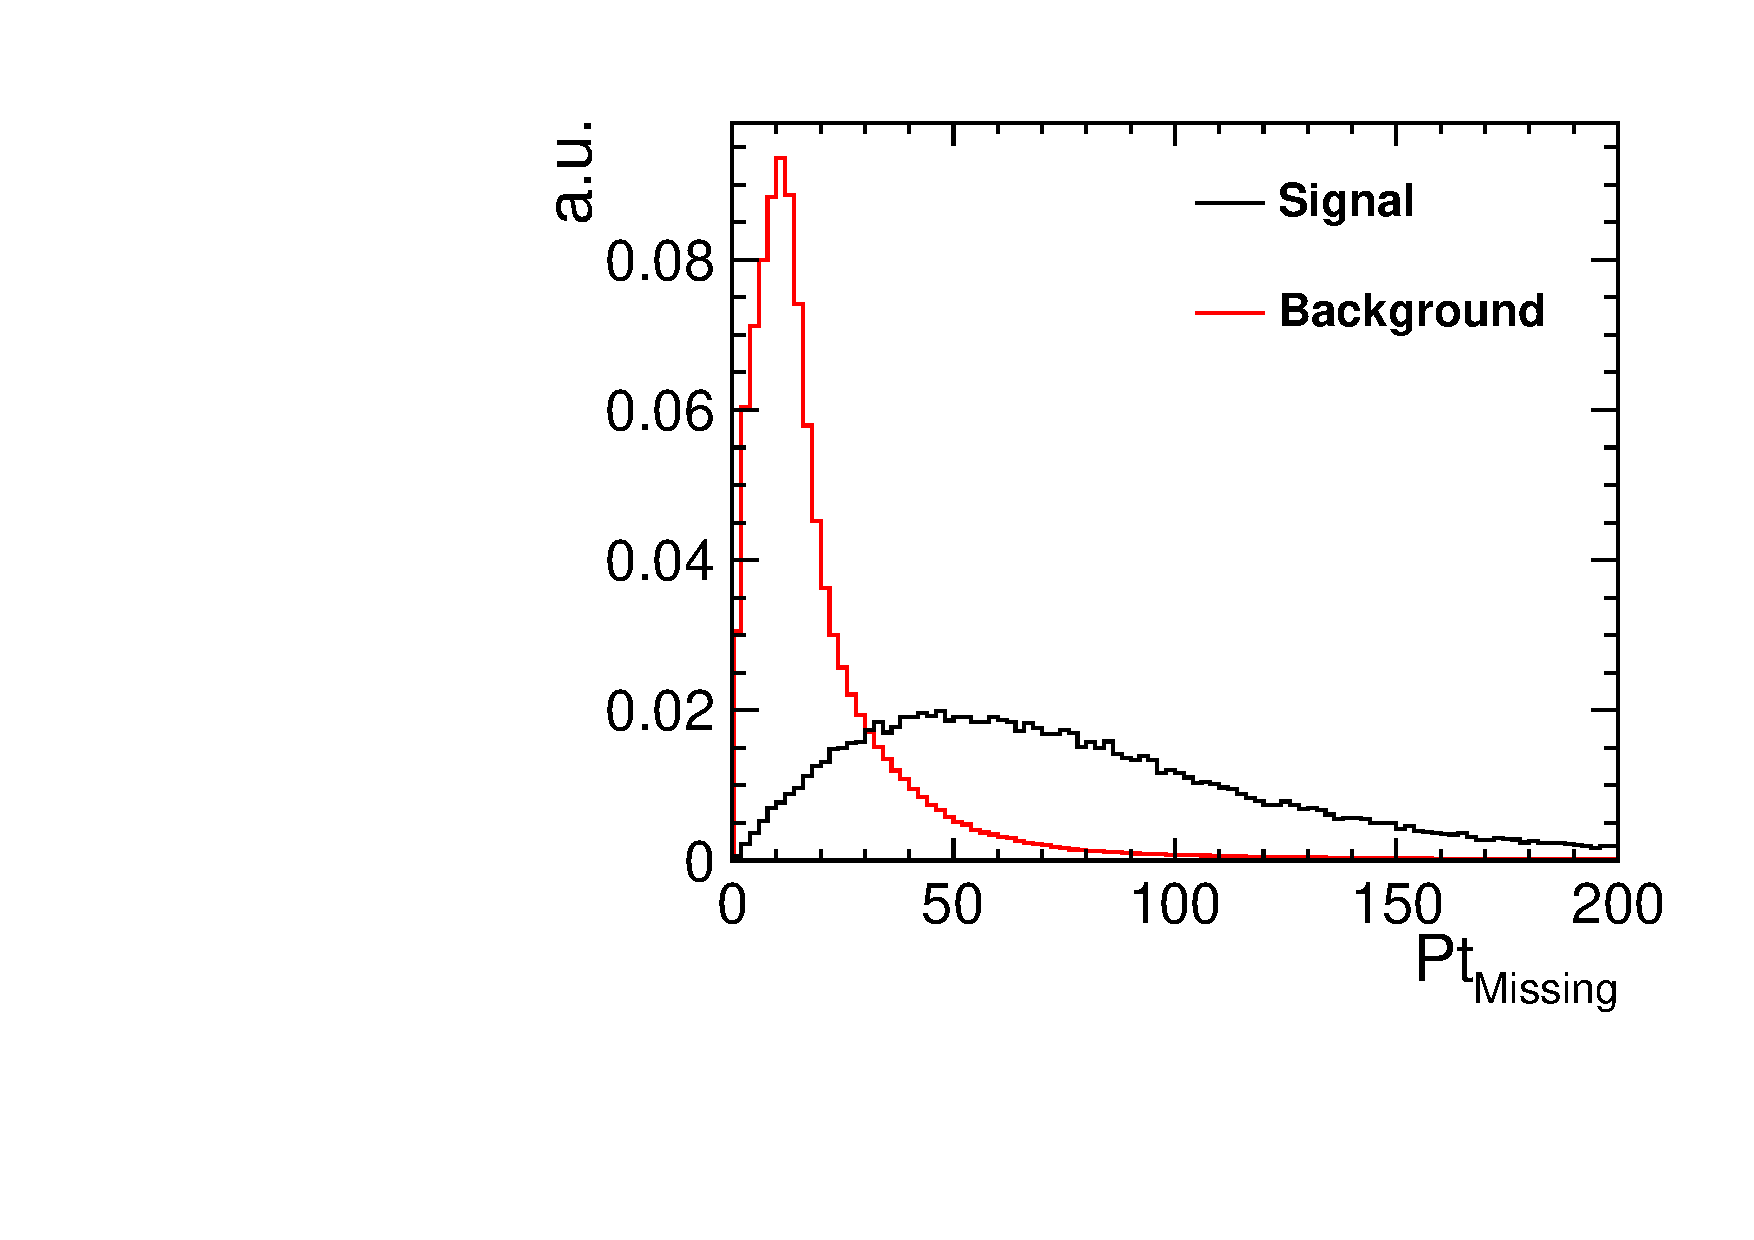
\includegraphics[width=0.75\linewidth]{Appendix/figures/MissingPt} 
    \caption{Missing transverse momentum} 
    \vspace{4ex}
  \end{subfigure}
\end{figure}

\begin{figure}[]\ContinuedFloat 
   \begin{subfigure}[]{0.5\linewidth}
    \centering
    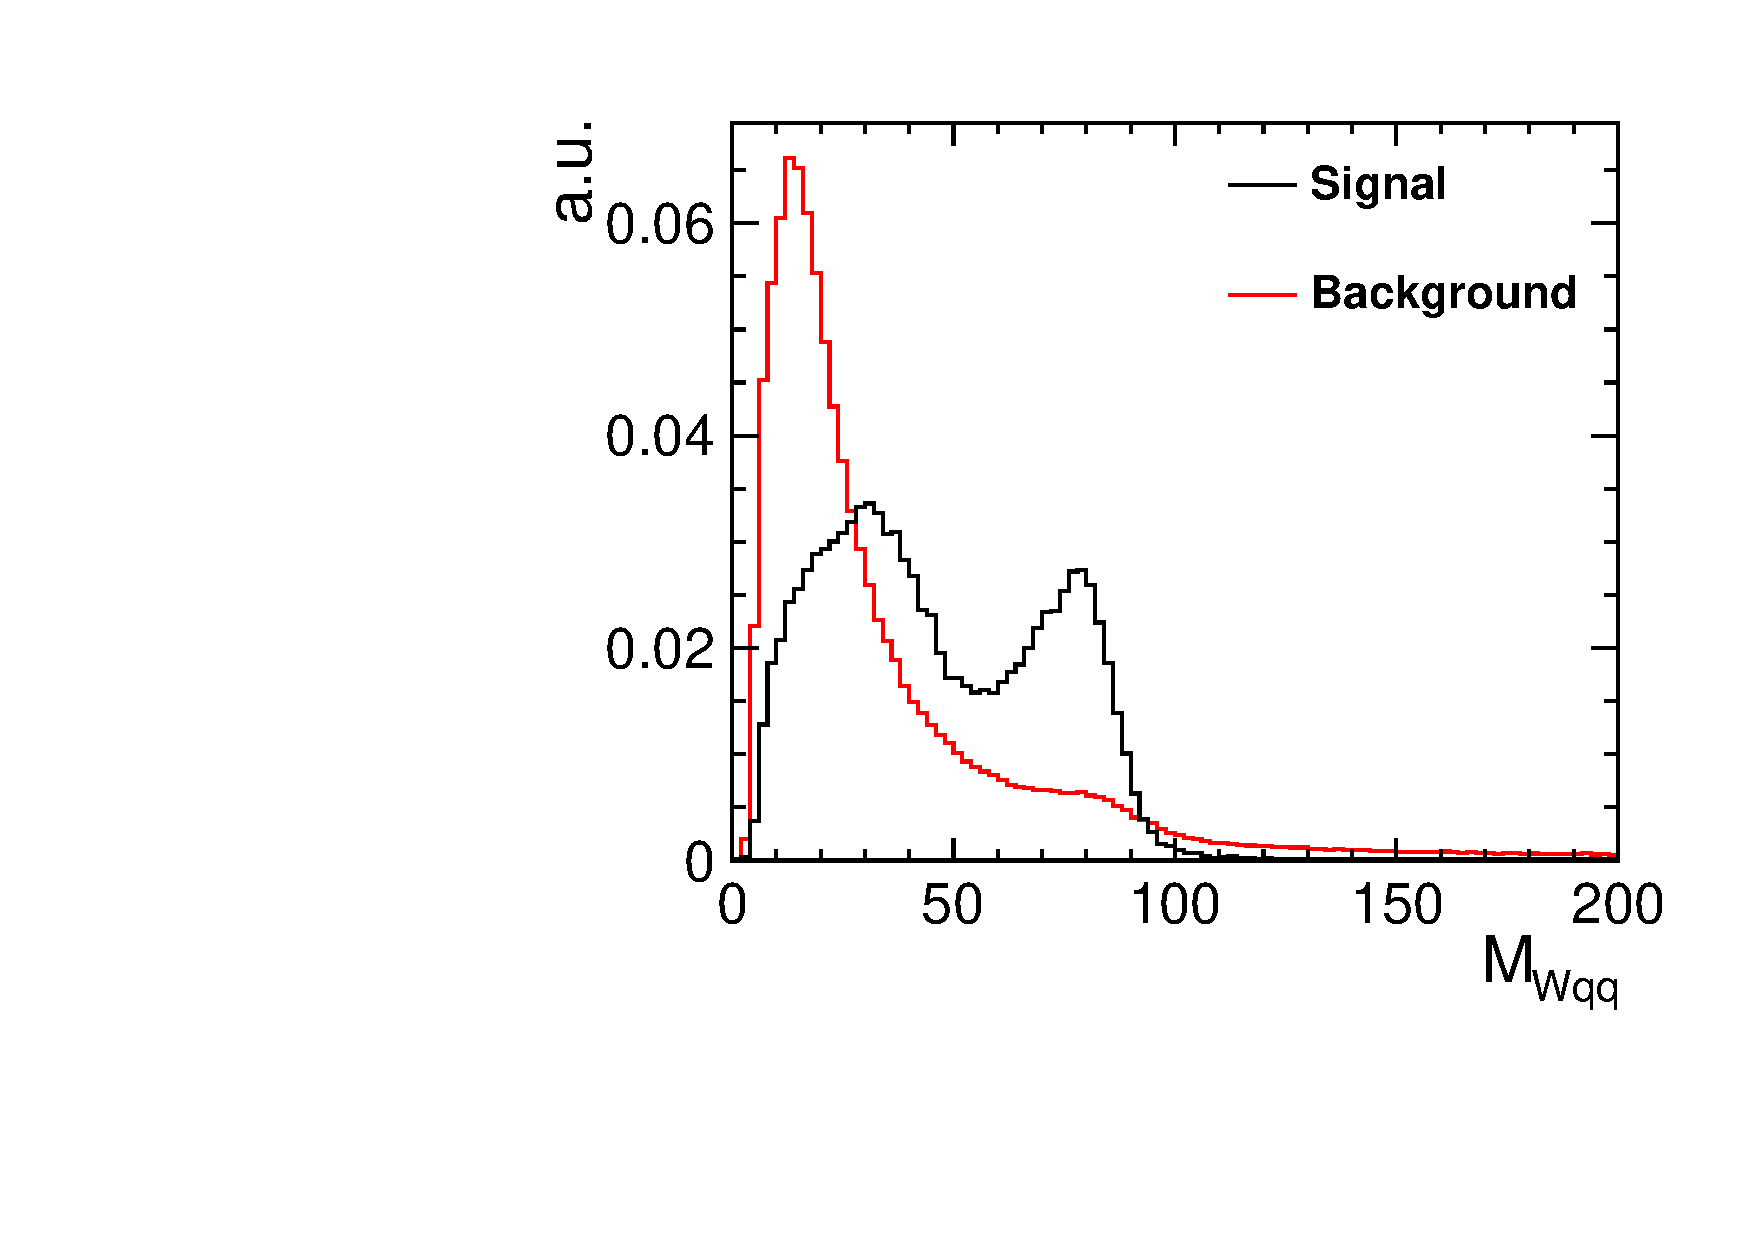
\includegraphics[width=0.75\linewidth]{Appendix/figures/MWqq} 
    \caption{Mass of hadronically decaying W} 
    \vspace{4ex}
  \end{subfigure}%%
  \begin{subfigure}[]{0.5\linewidth}
    \centering
    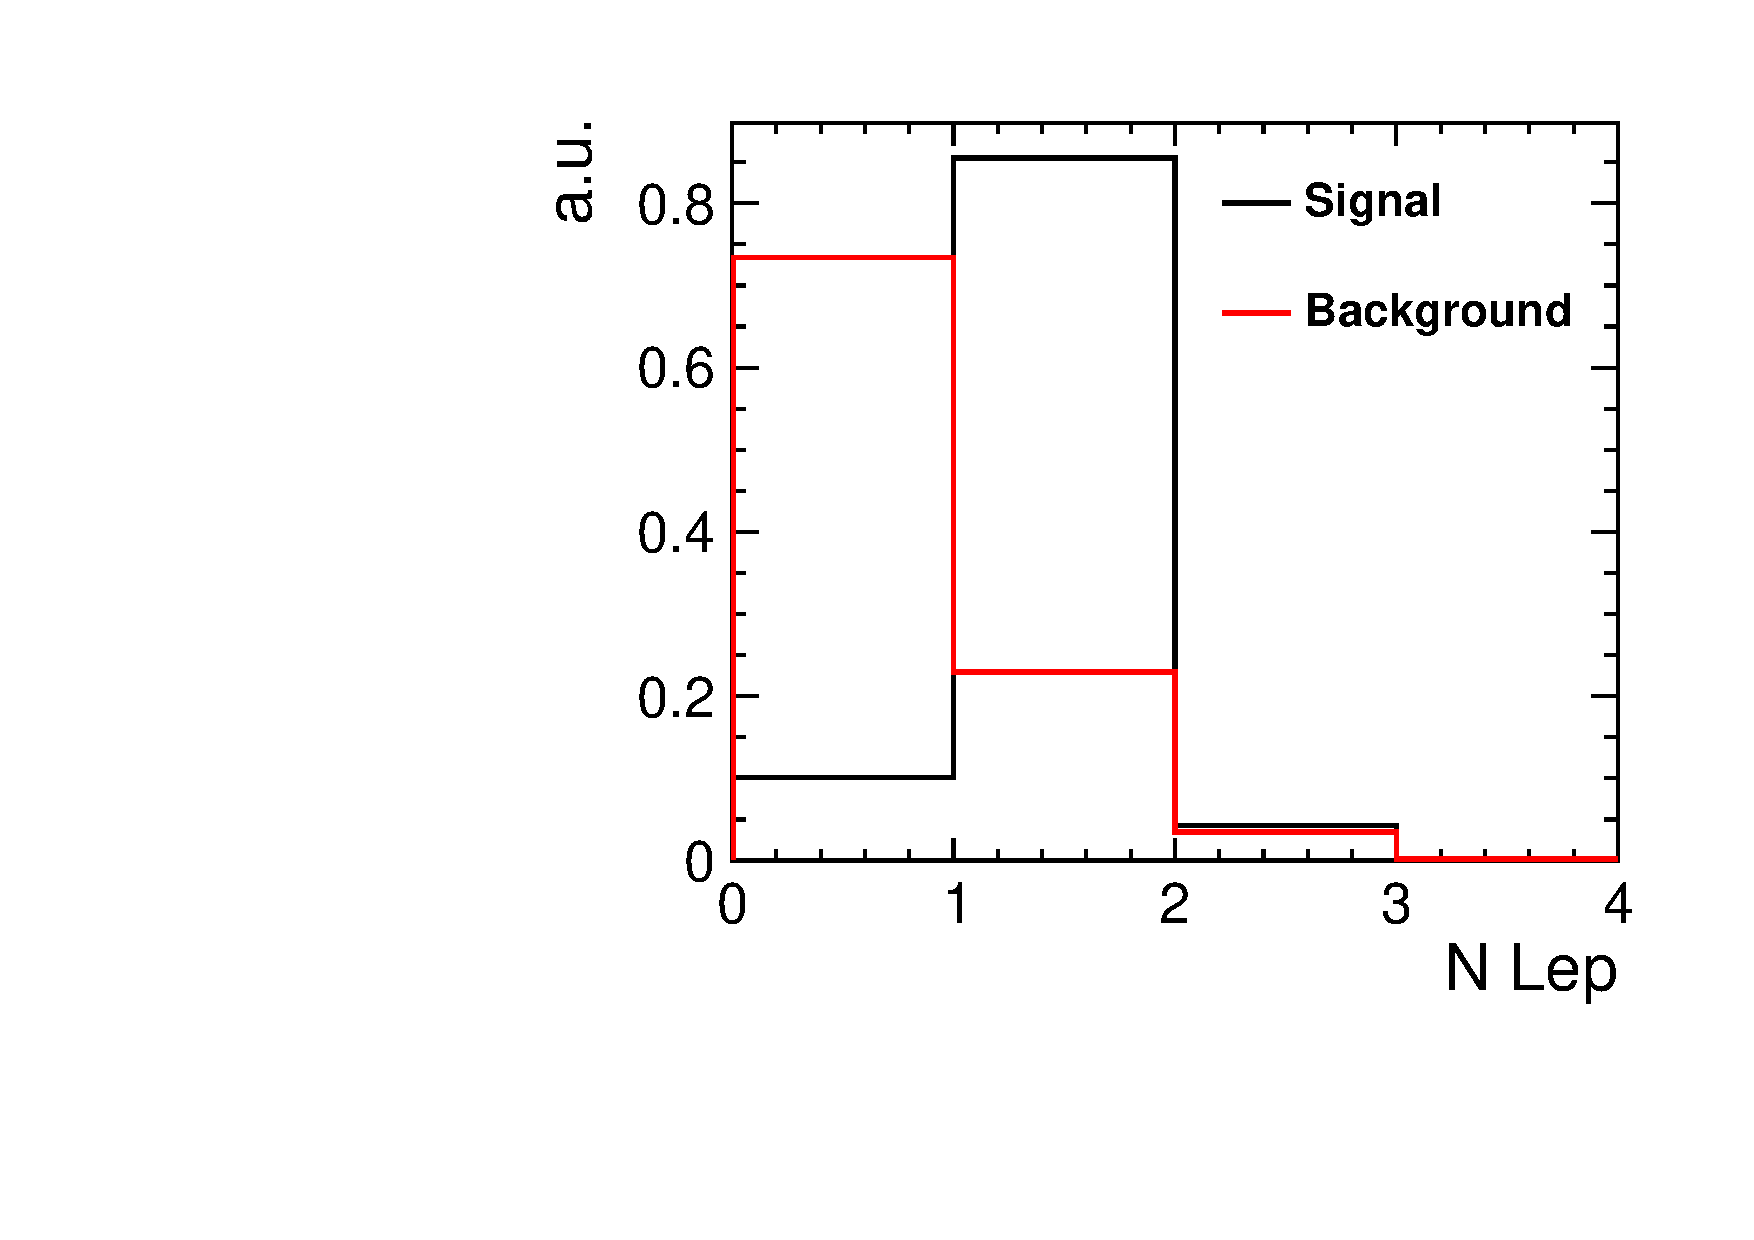
\includegraphics[width=0.75\linewidth]{Appendix/figures/nLep} 
    \caption{Number of reconstructed leptons} 
    \vspace{4ex}
  \end{subfigure}
  \begin{subfigure}[]{0.5\linewidth}
    \centering
    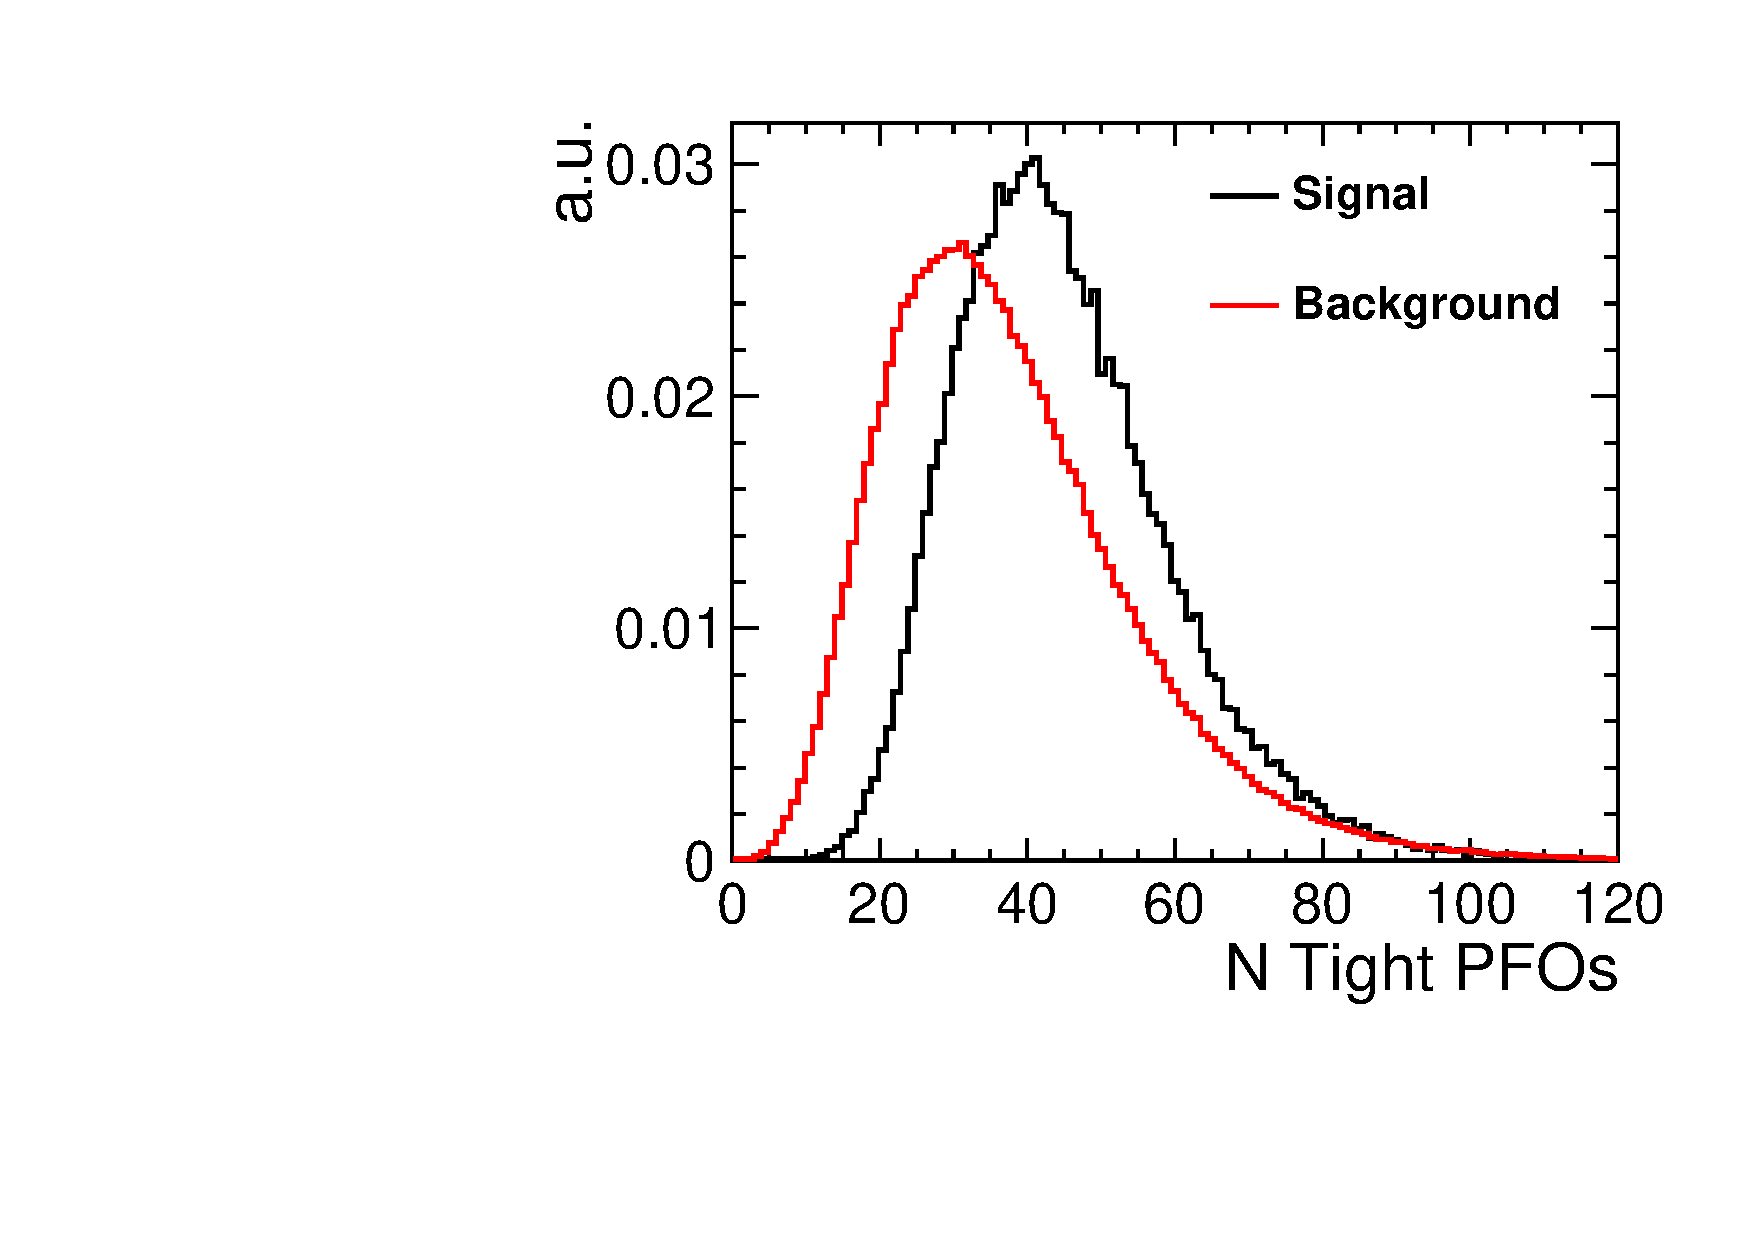
\includegraphics[width=0.75\linewidth]{Appendix/figures/NTightPFOs} 
    \caption{nPFOs passing tight timing cuts} 
    \vspace{4ex}
  \end{subfigure}%% 
  \begin{subfigure}[]{0.5\linewidth}
    \centering
    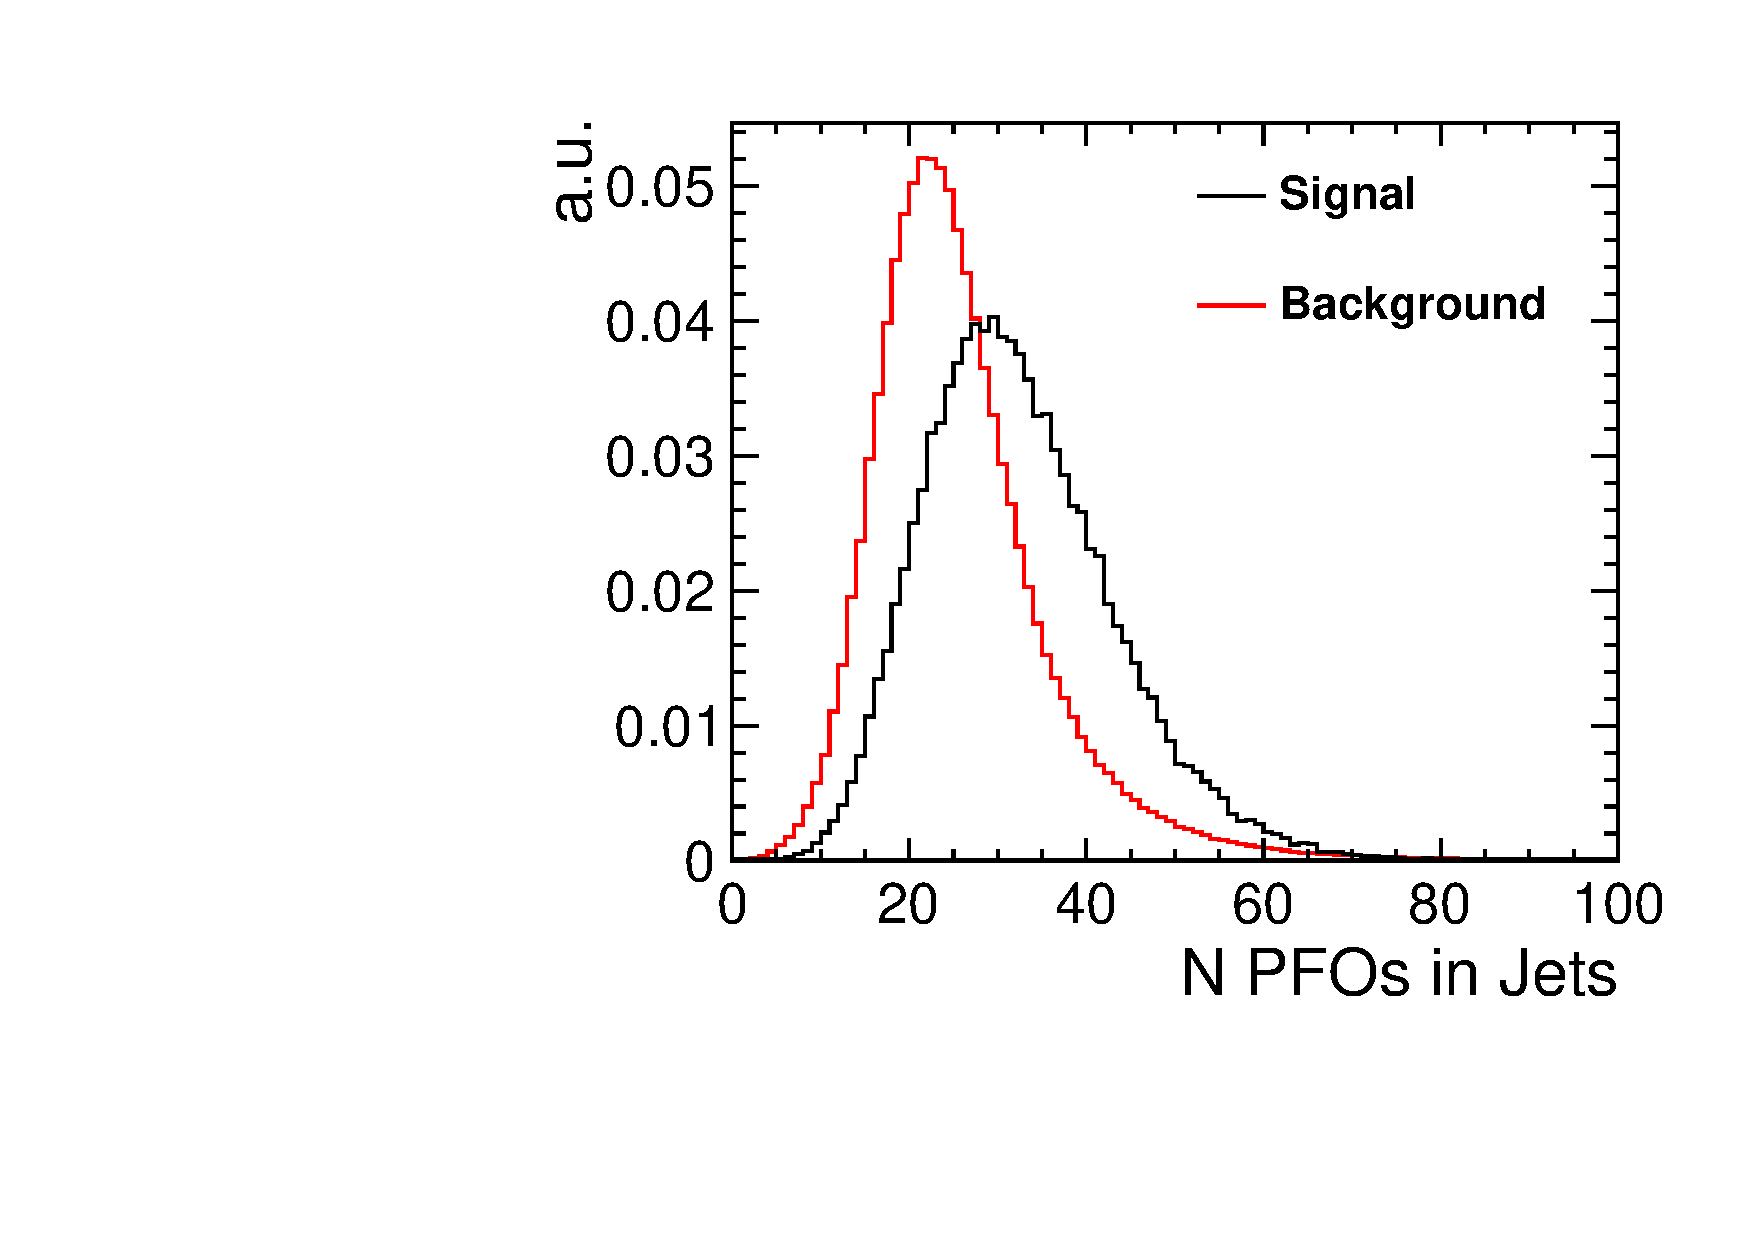
\includegraphics[width=0.75\linewidth]{Appendix/figures/PFOsInJets} 
    \caption{nPFOs assigned to jets} 
    \vspace{4ex}
  \end{subfigure} 
  \begin{subfigure}[]{0.5\linewidth}
    \centering
    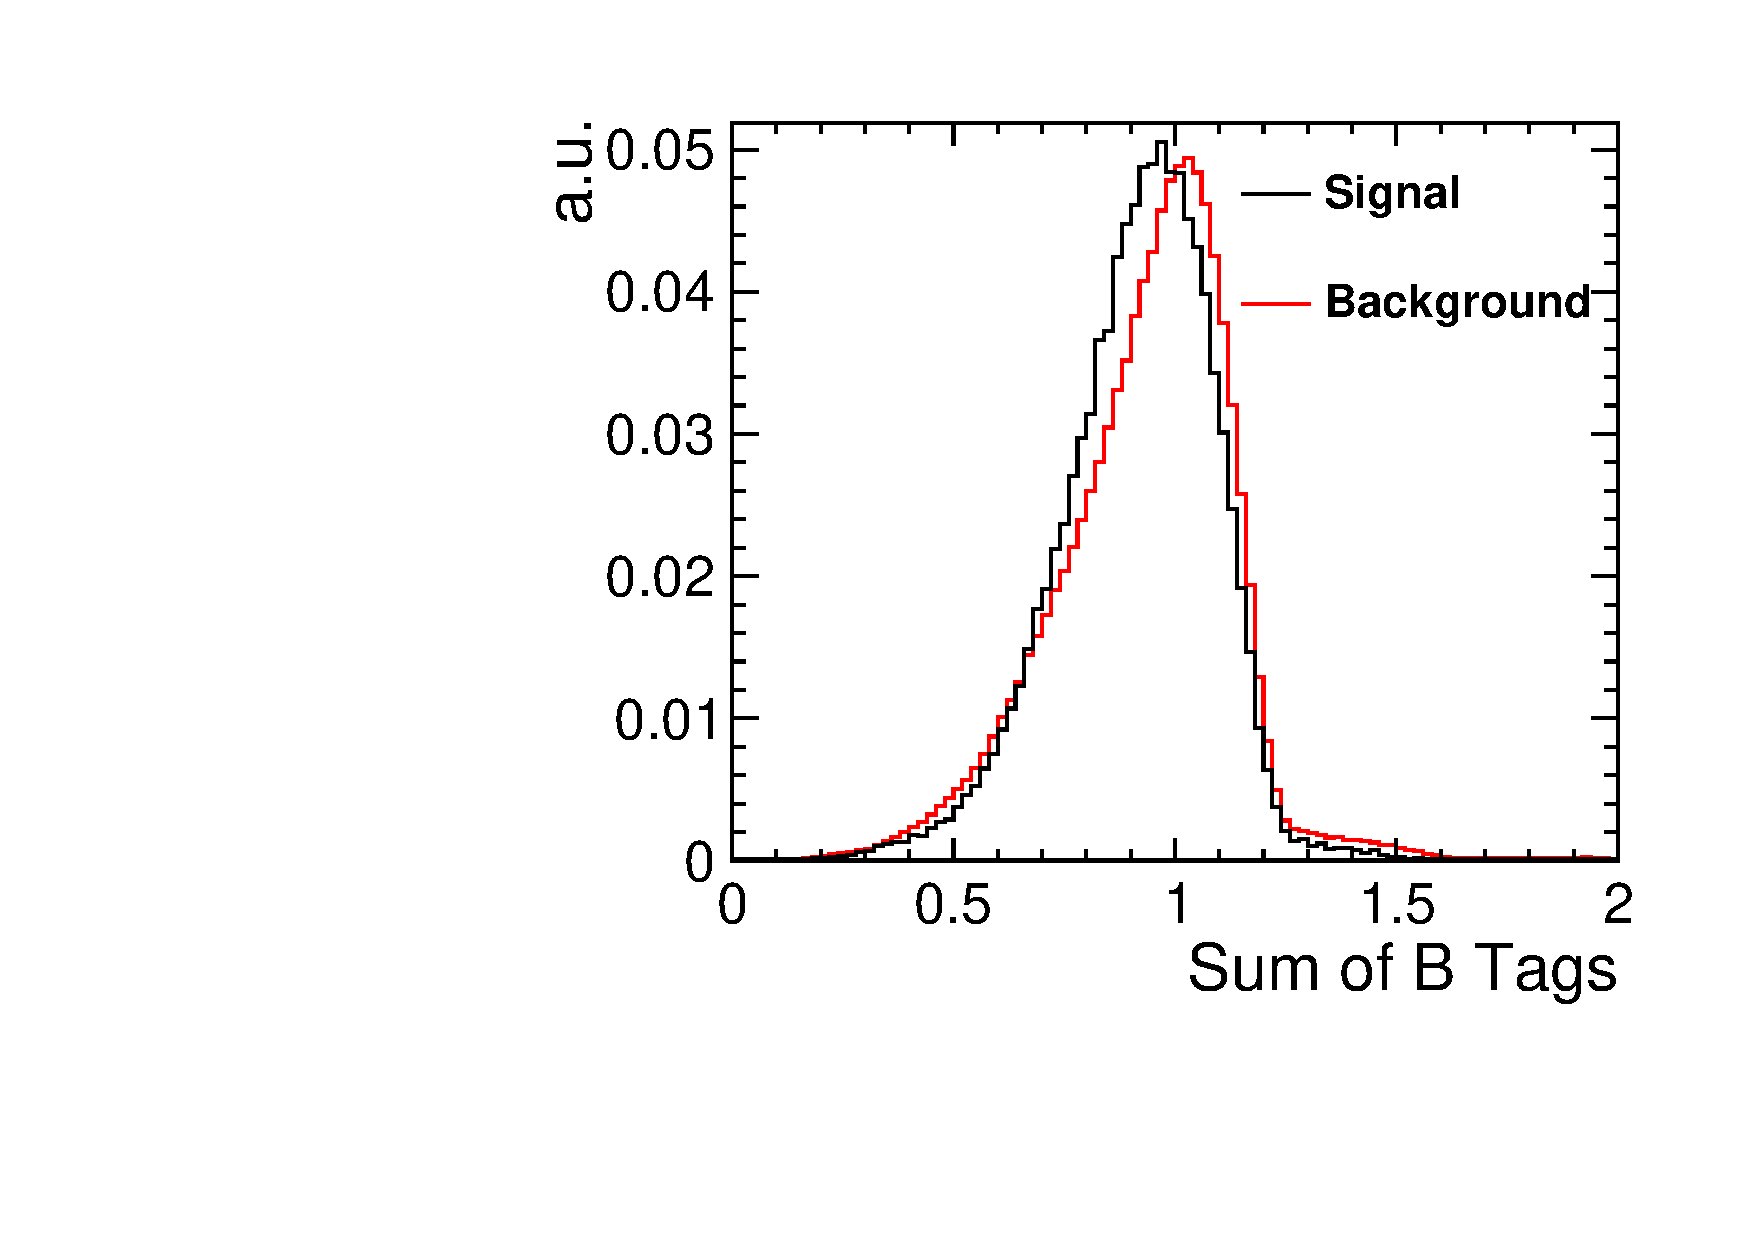
\includegraphics[width=0.75\linewidth]{Appendix/figures/SumBTags} 
    \caption{Sum of two highest b-tags} 
     \vspace{4ex}
 \end{subfigure}%%
  \begin{subfigure}[]{0.5\linewidth}
    \centering
    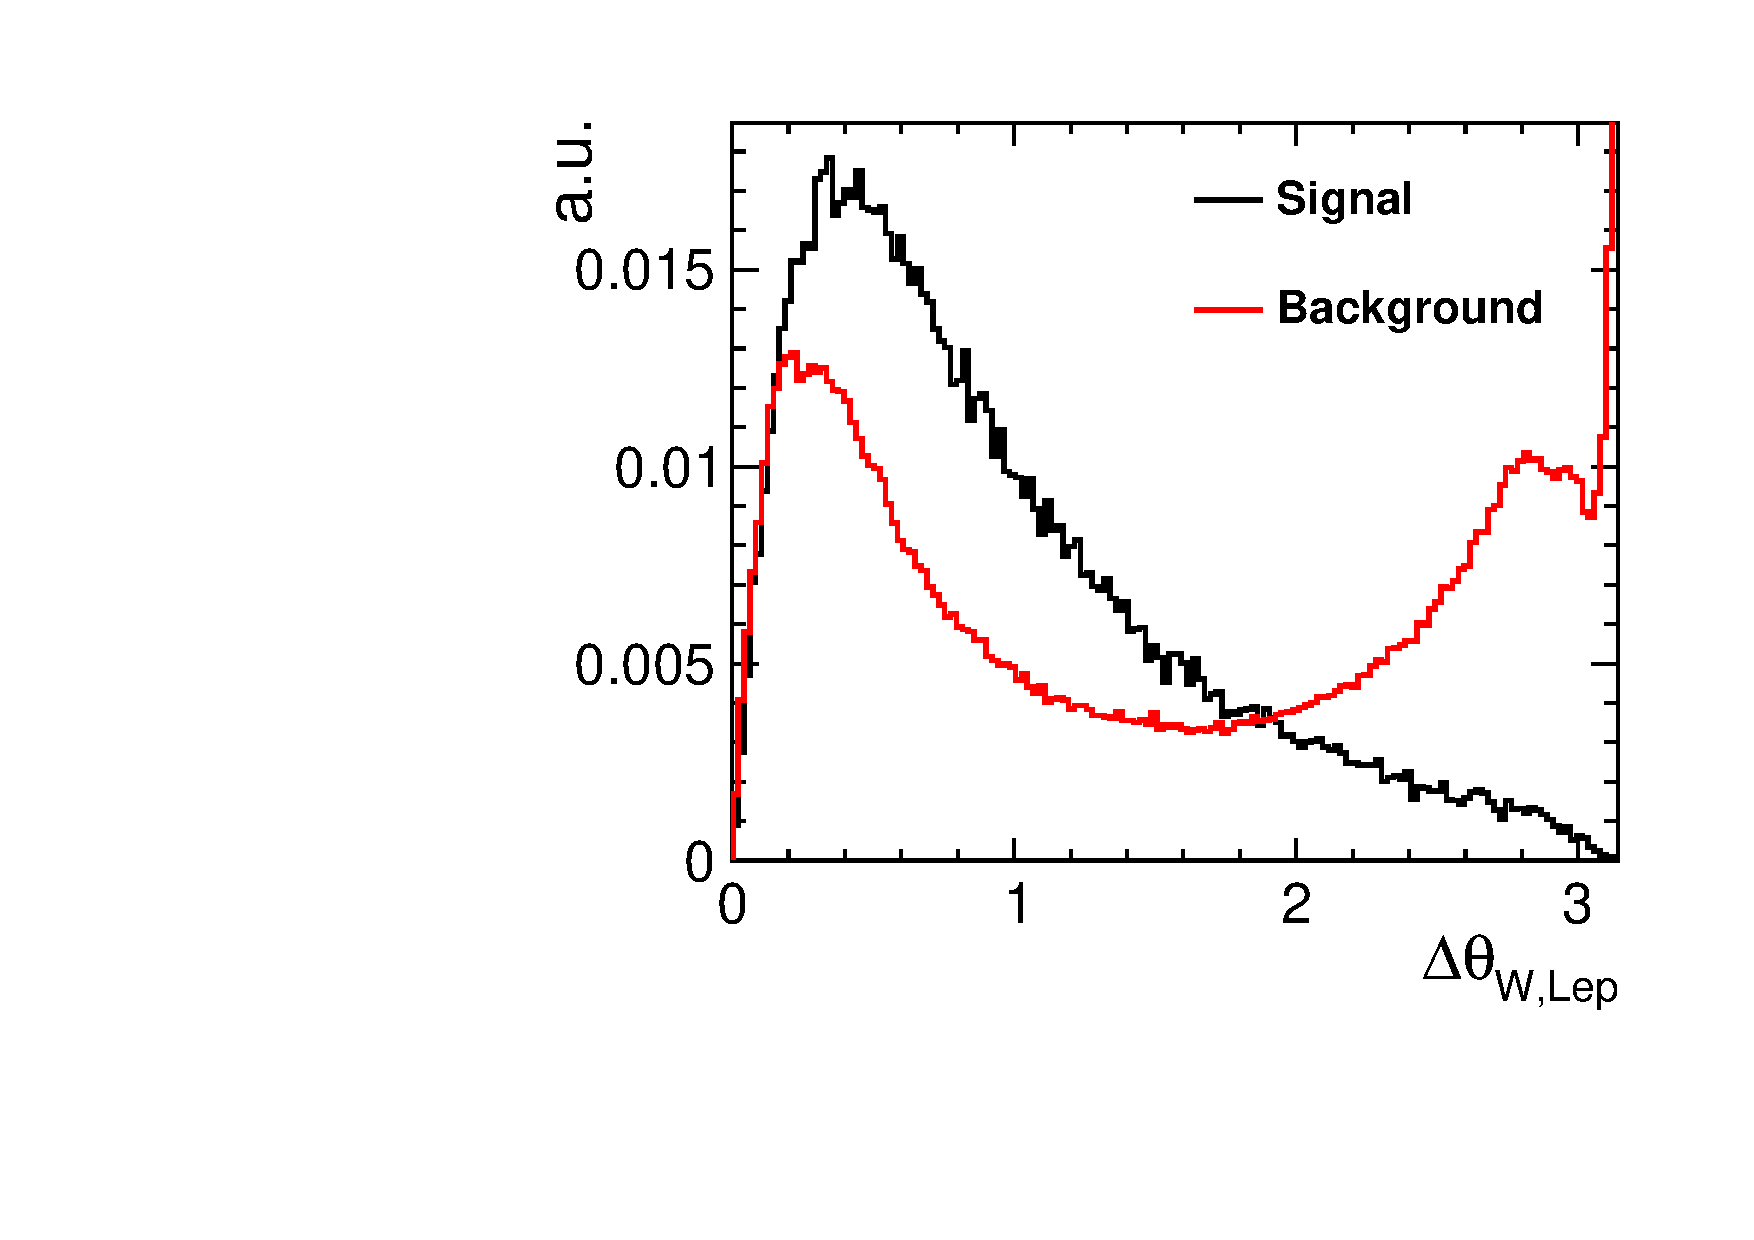
\includegraphics[width=0.75\linewidth]{Appendix/figures/WqqLepAngSep} 
    \caption{Angular Separation of the W and lepton} 
    \vspace{4ex}
  \end{subfigure}
  \begin{subfigure}[]{0.5\linewidth}
    \centering
    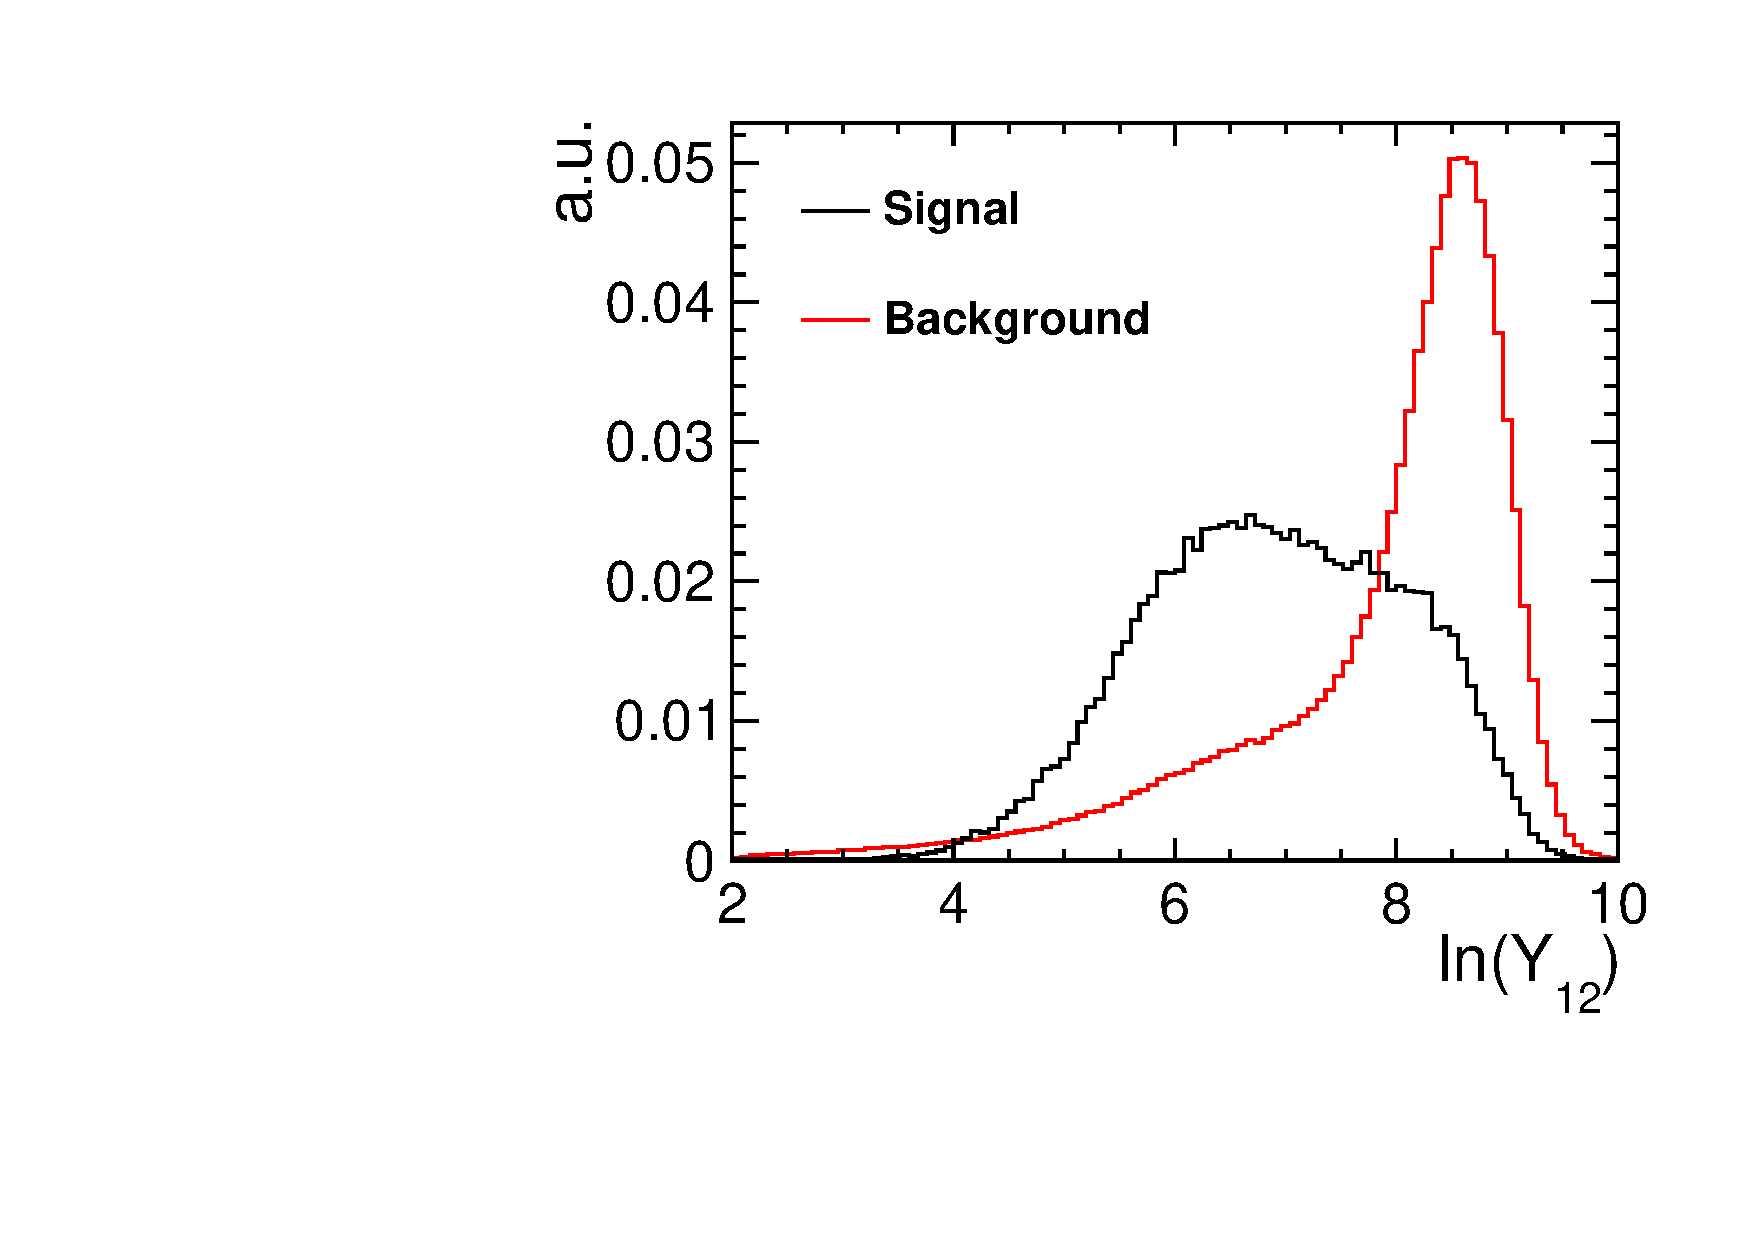
\includegraphics[width=0.75\linewidth]{Appendix/figures/Y12} 
    \caption{Jet Resolution Parameter Y$_{12}$} 
    \vspace{4ex}
  \end{subfigure}%%
\end{figure}


%%%%%%%%%% Appendix %%%%%%%%%%

\end{document} 
